\section{Path-dependent SSVI model}\label{sec:pdv_ssvi}
The present section is dedicated to the introduction of a new model for the joint dynamics of an implied volatility surface and the underlying asset price. The calibration results exposed in Section \ref{sec:ssvi} demonstrate the ability of a particular case of the SSVI parameterization - the parsimonious SSVI - to fit reasonably well historical implied volatility surfaces while guaranteeing the absence of static arbitrage with only 4 parameters. As a consequence, we propose to specify our model as a dynamic version of the parsimonious SSVI: each parameter of the parsimonious SSVI is considered as a stochastic process whose dynamics remains to be determined. One option to jointly model the evolution of the parsimonious SSVI parameters and the underlying asset would be to introduce a correlation between the random noises driving each process. However, in view of the empirical study conducted in Section \ref{sec:empirical_study} which indicates that there is a feedback effect of the past returns and the past squared returns of the underlying index price onto the level of the ATM implied volatility, we prefer another option. Instead of using a correlation, the idea is to explicitly model the response of each of the 4 parameters to the evolution of the underlying asset price. To this end, we measure to which extent the trend feature and the volatility feature of the path-dependent volatility (PDV) model presented in Section \ref{sec:pdv_model} allow to explain the variations of the 4 parameters of the parsimonious SSVI model. This study is presented in Section \ref{sec:pdv_ssvi_params} below. Then, Section \ref{sec:dynamics_specification} introduces the dynamics of the asset price and of the parsimonious SSVI parameters. Finally, Section \ref{sec:model_calibration} and \ref{sec:num_results} detail the calibration and the simulation of the model. \\

\begin{remark}
    It is important to note at this stage that there should be some consistency between the dynamics of the implied volatility surface and the one of the underlying asset price to prevent dynamic arbitrages. More precisely, the process $t\mapsto C_{BS}(K,T,S_t,IV_t(K,T))$, where $C_{BS}$ is the Black-Scholes price of a call option of strike $K$ and maturity $T$ when the spot price is $S_t$ and the implied volatility is $IV_t(K,T)$, should be a martingale. Several authors (e.g. \citeauthor{schonbucher1999marketmodel}, \citeyear{schonbucher1999marketmodel}, \citeauthor{schweizer2008term}, \citeyear{schweizer2008term}, \citeauthor{jacod2010risk}, \citeyear{jacod2010risk}) found conditions guaranteeing the existence of a joint model satisfying the absence of dynamic arbitrage in various settings. However, these conditions are not tractable and we are not aware of any parametric model satisfying those. \cite{amrani2021dynamics} find a necessary condition guaranteeing the absence of dynamic arbitrage for a dynamic version of the SSVI parameterization but this condition is very restrictive. Thus, due to the difficulty of designing a joint model which does not exhibit dynamic arbitrages, we do not look for such a model and we focus on finding one which is as consistent as possible with historical data and which does not exhibit static arbitrages. 
\end{remark}


\subsection{Path-dependency of the parsimonious SSVI parameters}\label{sec:pdv_ssvi_params}
The calibration of the parsimonious SSVI in Section \ref{sec:pssvi} provides the daily evolutions of the parameters $a$, $p$, $\rho$ and $\eta$. Based on these daily evolutions, we can calibrate the PDV model (\ref{eq:guyon_model}) where we replace $\text{Volatility}_t$ in Equation (\ref{eq:guyon_model}) by each parameter of the parsimonious SSVI. Note that we consider the logarithm of $p$ instead of $p$ in the PDV model since we observed that this provides a better fit. The calibration methodology is the same as the one exposed in Section \ref{sec:calib_meth}. We refer to Appendix \ref{sec:hyperparams_ssvi for the estimation method of the hyperparameters of the PDV model and their values}. The $R^2$ scores obtained on the train and the test sets for each parameter and for each index are reported in Table \ref{tab:ssvi_r2_scores}. On the one hand, these results show that the time evolution of the parameter $a$ is well explained by the evolution of the underlying asset price both on the train and the test sets, which is line with the results obtained for the ATM implied volatility since $a$ captures the ATM total variance level (whose evolution is similar to the one of the ATM implied volatility and as such we expect the study conducted in Section \ref{sec:empirical_study_numerical_results} to be still valid for the ATM total variance). The same observation holds for $p$. However the fact that the PDV model works well for $p$ was not anticipated as it allows to parameterize how the ATM total variance increases with the time-to-maturity and it is not homogenous to the ATM total variance level. Thus, we emphasize that this is a key finding. On the other hand, the $R^2$ scores for the parameters $\rho$ and $\eta$ are decent on the train set but small or negative on the test set. This indicates that the trend and the volatility features are not good predictors for these two parameters. Let us however point out that the evolution of these two parameters does not appear as completely independent from the one of the underlying asset price as one can see in Figure \ref{fig:rho_eta_evolution}. In particular, we see a large variations of these parameters during the market drop of March 2020. Despite this, we did not find features allowing a good prediction (i.e. material $R^2$ scores on the test set) of $\rho$ and $\eta$ (we tried for example skewness, kurtosis and correlation features). As a consequence, the Browian motions of these parameters will only be correlated to the Brownian motion of the asset price. 

\begin{remark}
    $\rho$ and $\eta$ parameterize respectively the orientation and the convexity of the implied volatility smile as illustrated in Figure \ref{fig:influence_rho_eta}.
\end{remark}


\begin{figure}[h]   
    \centering
    \subfigure[$\rho$]{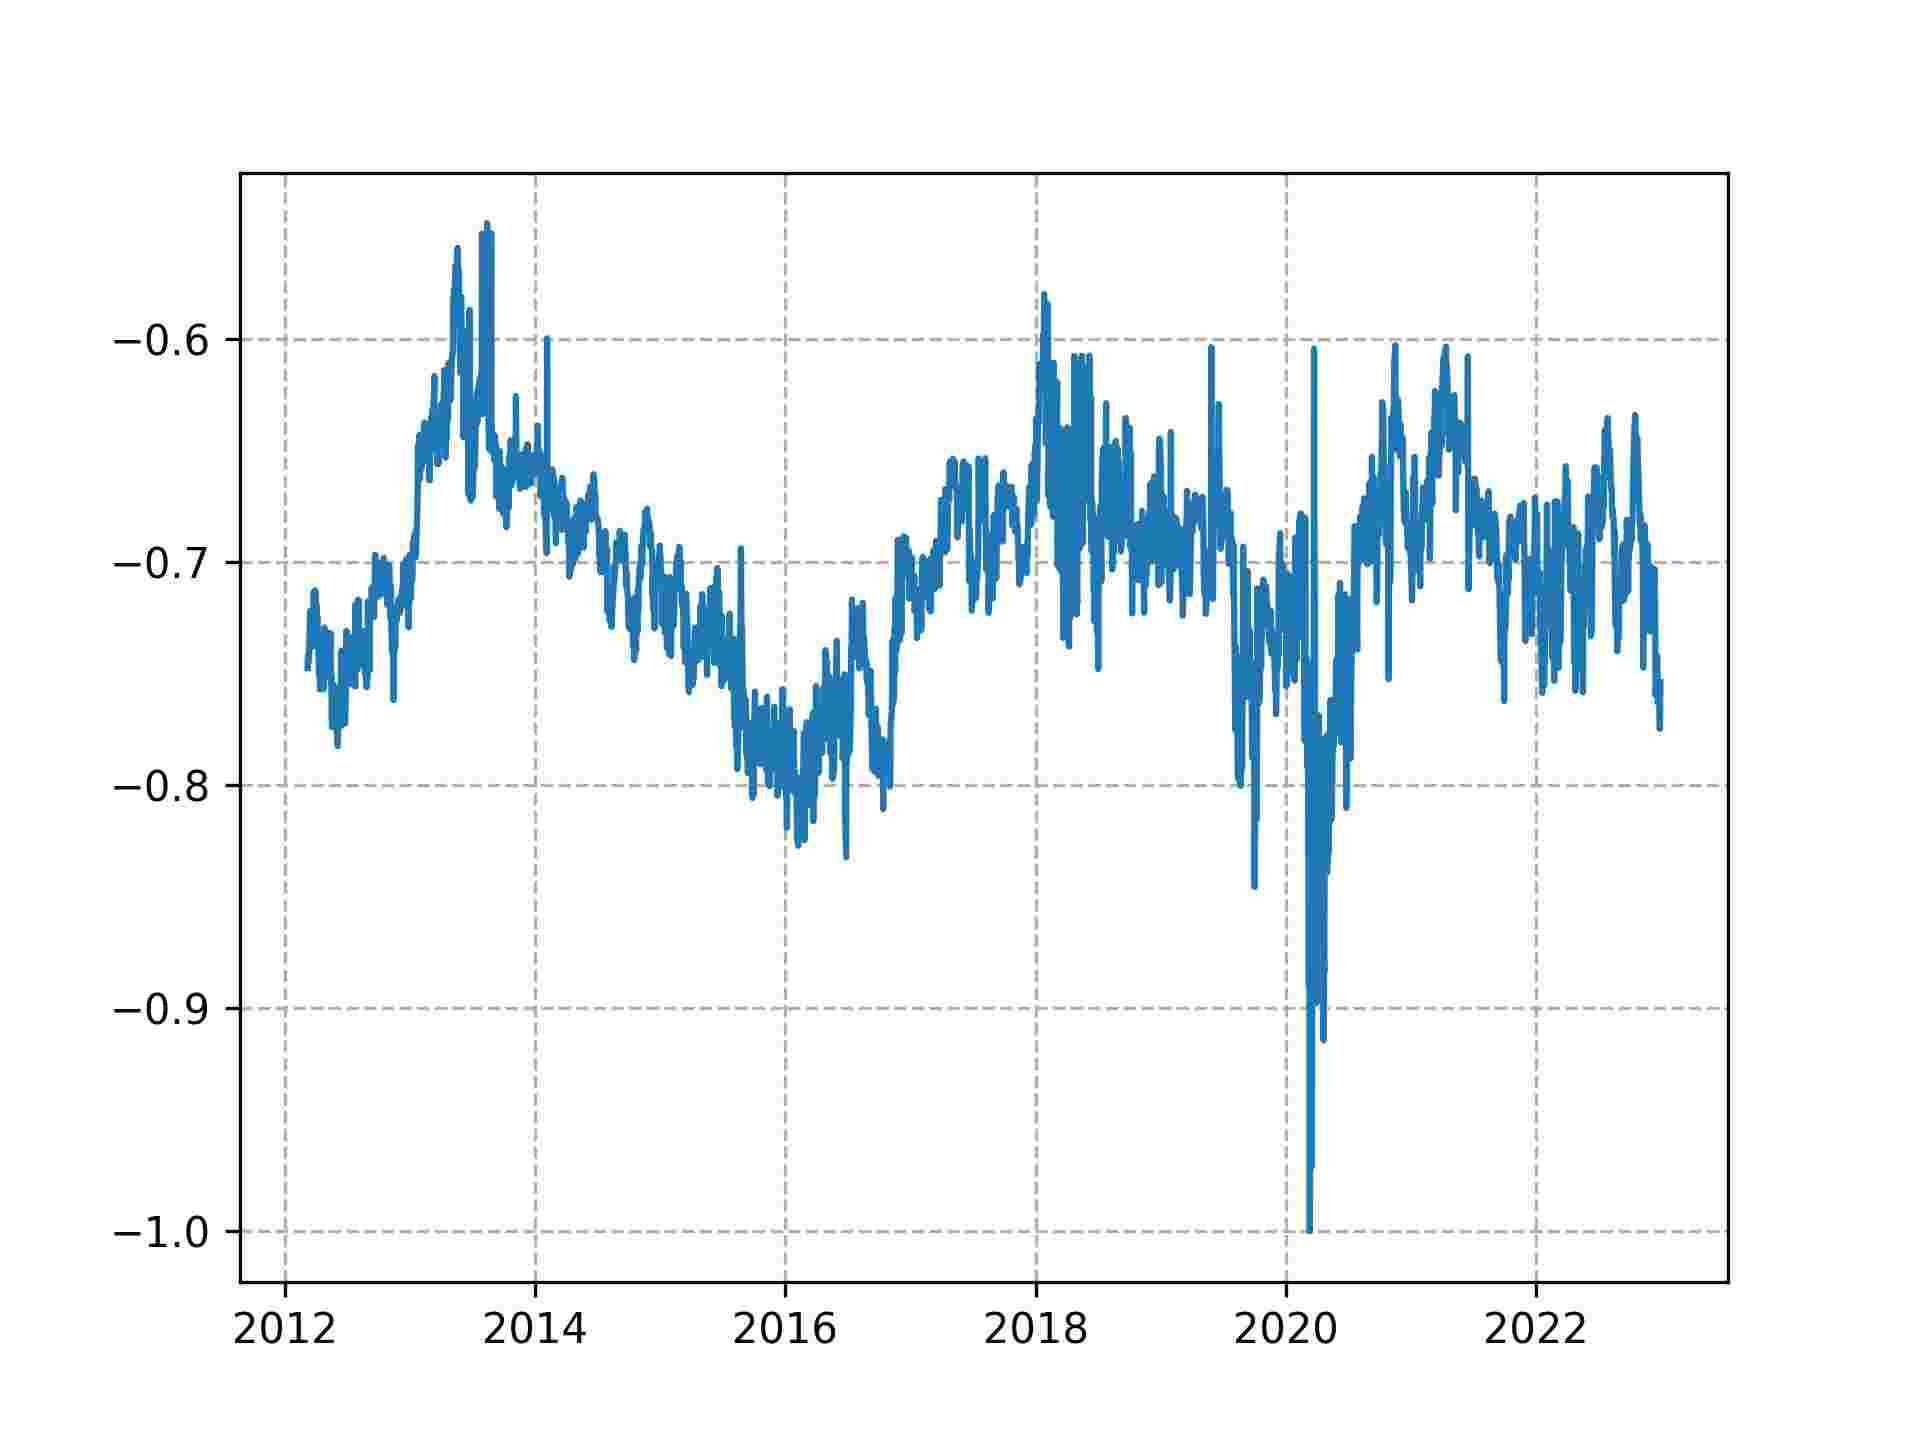
\includegraphics[width=0.45\linewidth]{rho_Evolution.jpg}}
    \subfigure[$\eta$]{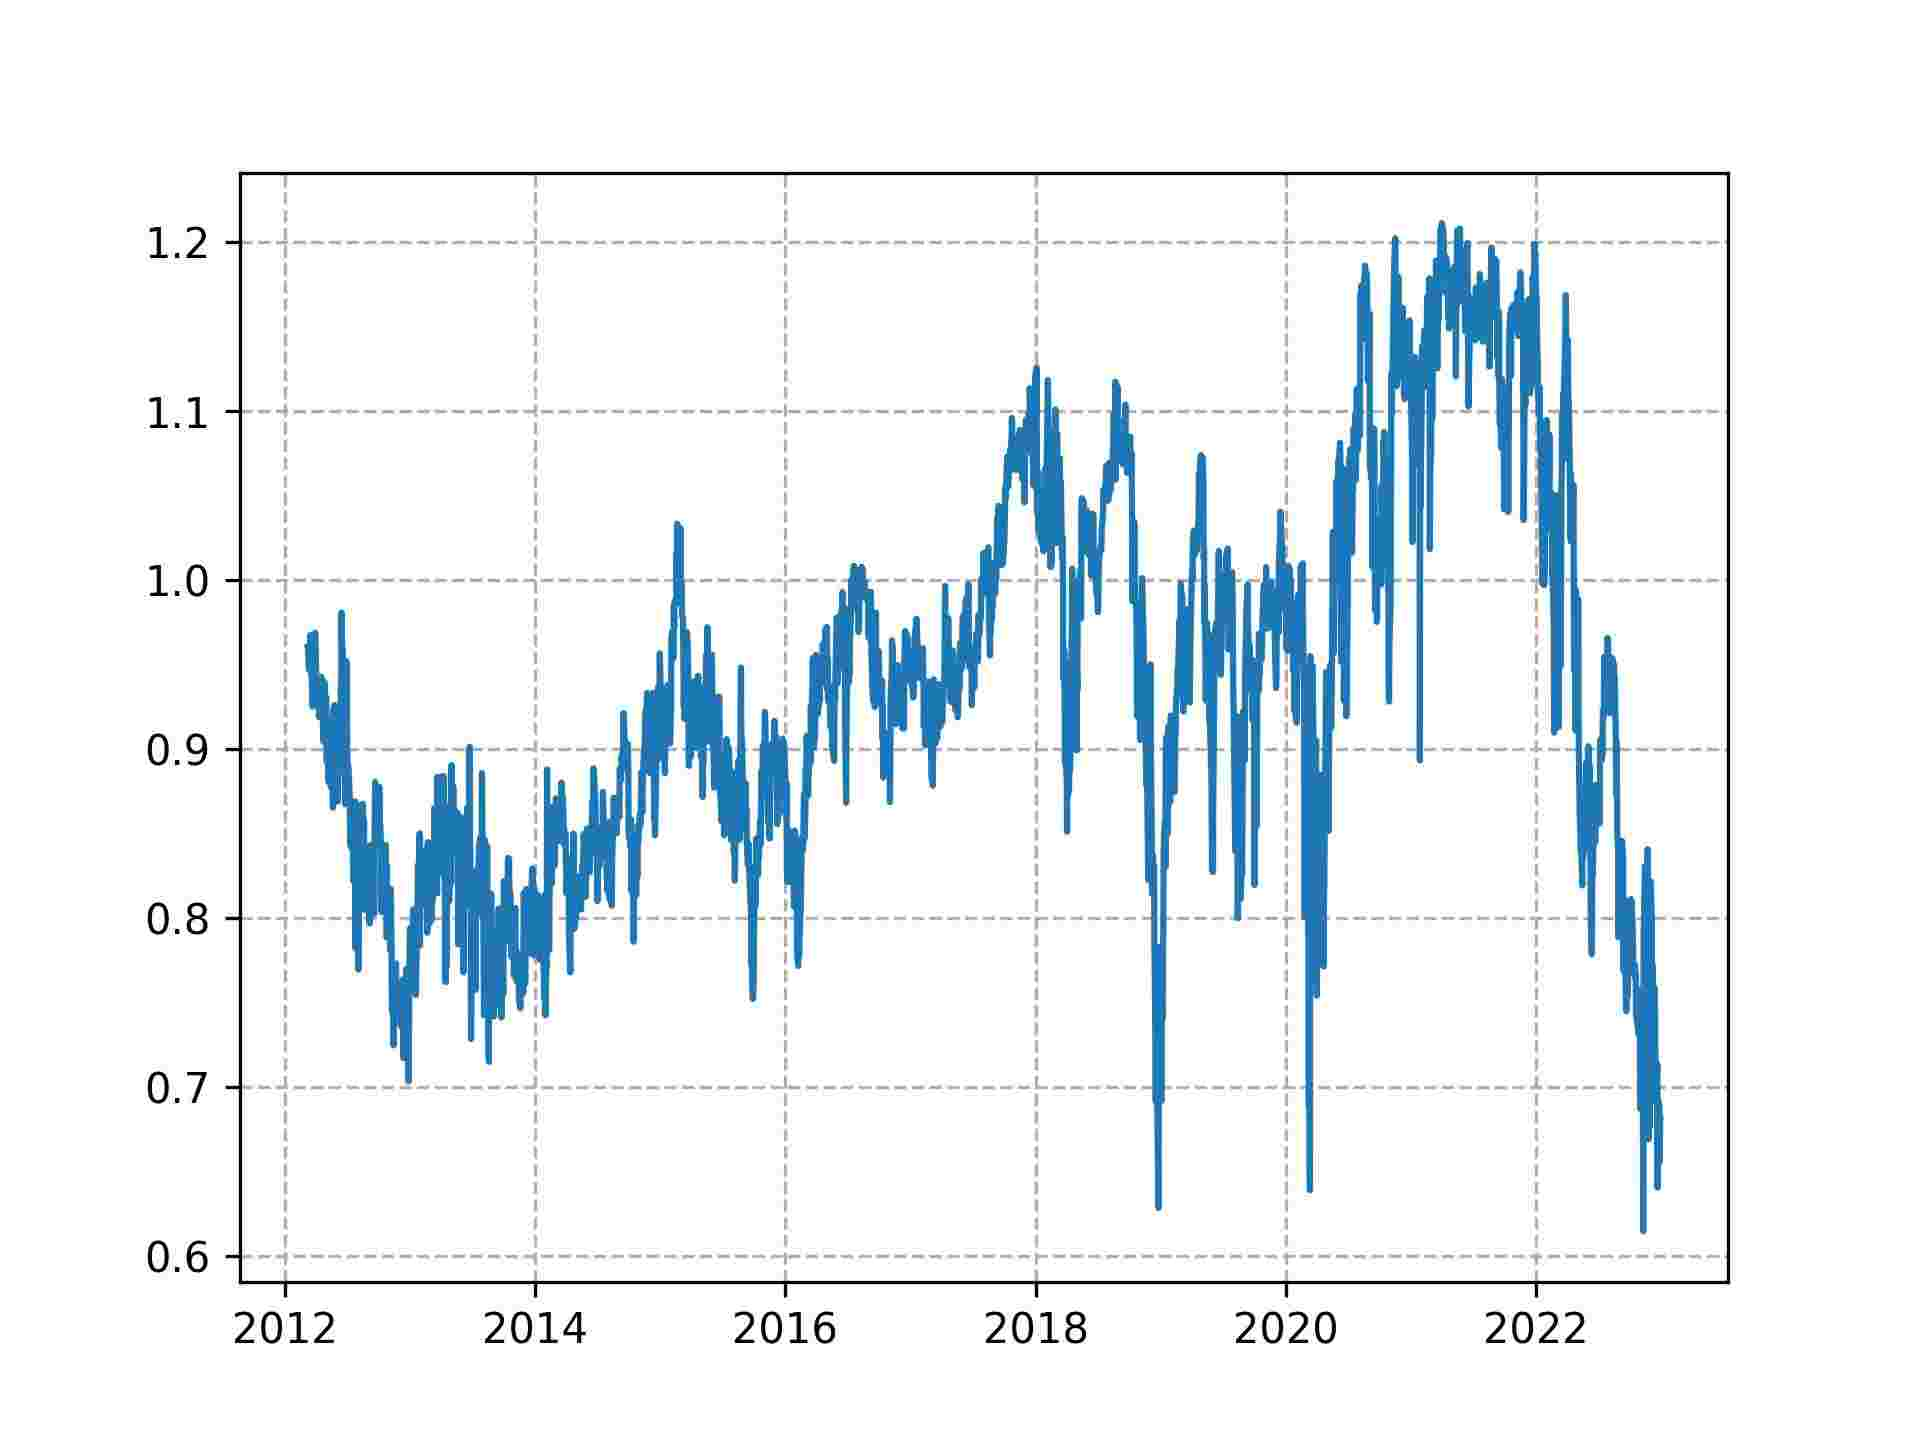
\includegraphics[width=0.45\linewidth]{eta_Evolution.jpg}}
    \caption{Historical evolution of the $\rho$ and $\eta$ parameters.}
    \label{fig:rho_eta_evolution}
\end{figure}

\begin{remark}
    \cite{guyon2022volatility} and \cite{gazzani2024pricing} considered a third feature given by $R_1^2 \mathbb{1}_{\{R_1\ge 0\}}$ in the PDV model in order to achieve a satisfying joint SPX/VIX fit. Adding this feature to explain the variations of our 4 parameters does not improve the $R^2$ scores.  \\
\end{remark}

\begin{table}[h]
    \centering
    \caption{$R^2$ scores of the PDV model on the parameters of the parsimonious SSVI on the train and the test sets.}
    \label{tab:ssvi_r2_scores}
    \begin{tabular}{@{}ccccccc@{}}
    \toprule
    & \multicolumn{2}{c}{S\&P 500} & \multicolumn{2}{c}{Euro Stoxx 50} \\ \toprule
        &  Train & Test &  Train & Test   \\ \midrule
    $a$   &    93.7\% & 72.9\%        & 85.7\% & 49.4\%    \\
    $p$   &    76.2\%    & 47.0\% &    76.3\%    & 75.3\%    \\
    $\rho$ &    50.7\%    & -400.1\%    &  35.9\%    & 19.7\%    \\
    $\eta$ &    63.6\%    & 18.6\%    &   58.0\%    & -899.5\%    \\ \bottomrule
\end{tabular}
\end{table}

\begin{figure}[h]   
    \centering
    \subfigure[Influence of $\rho$]{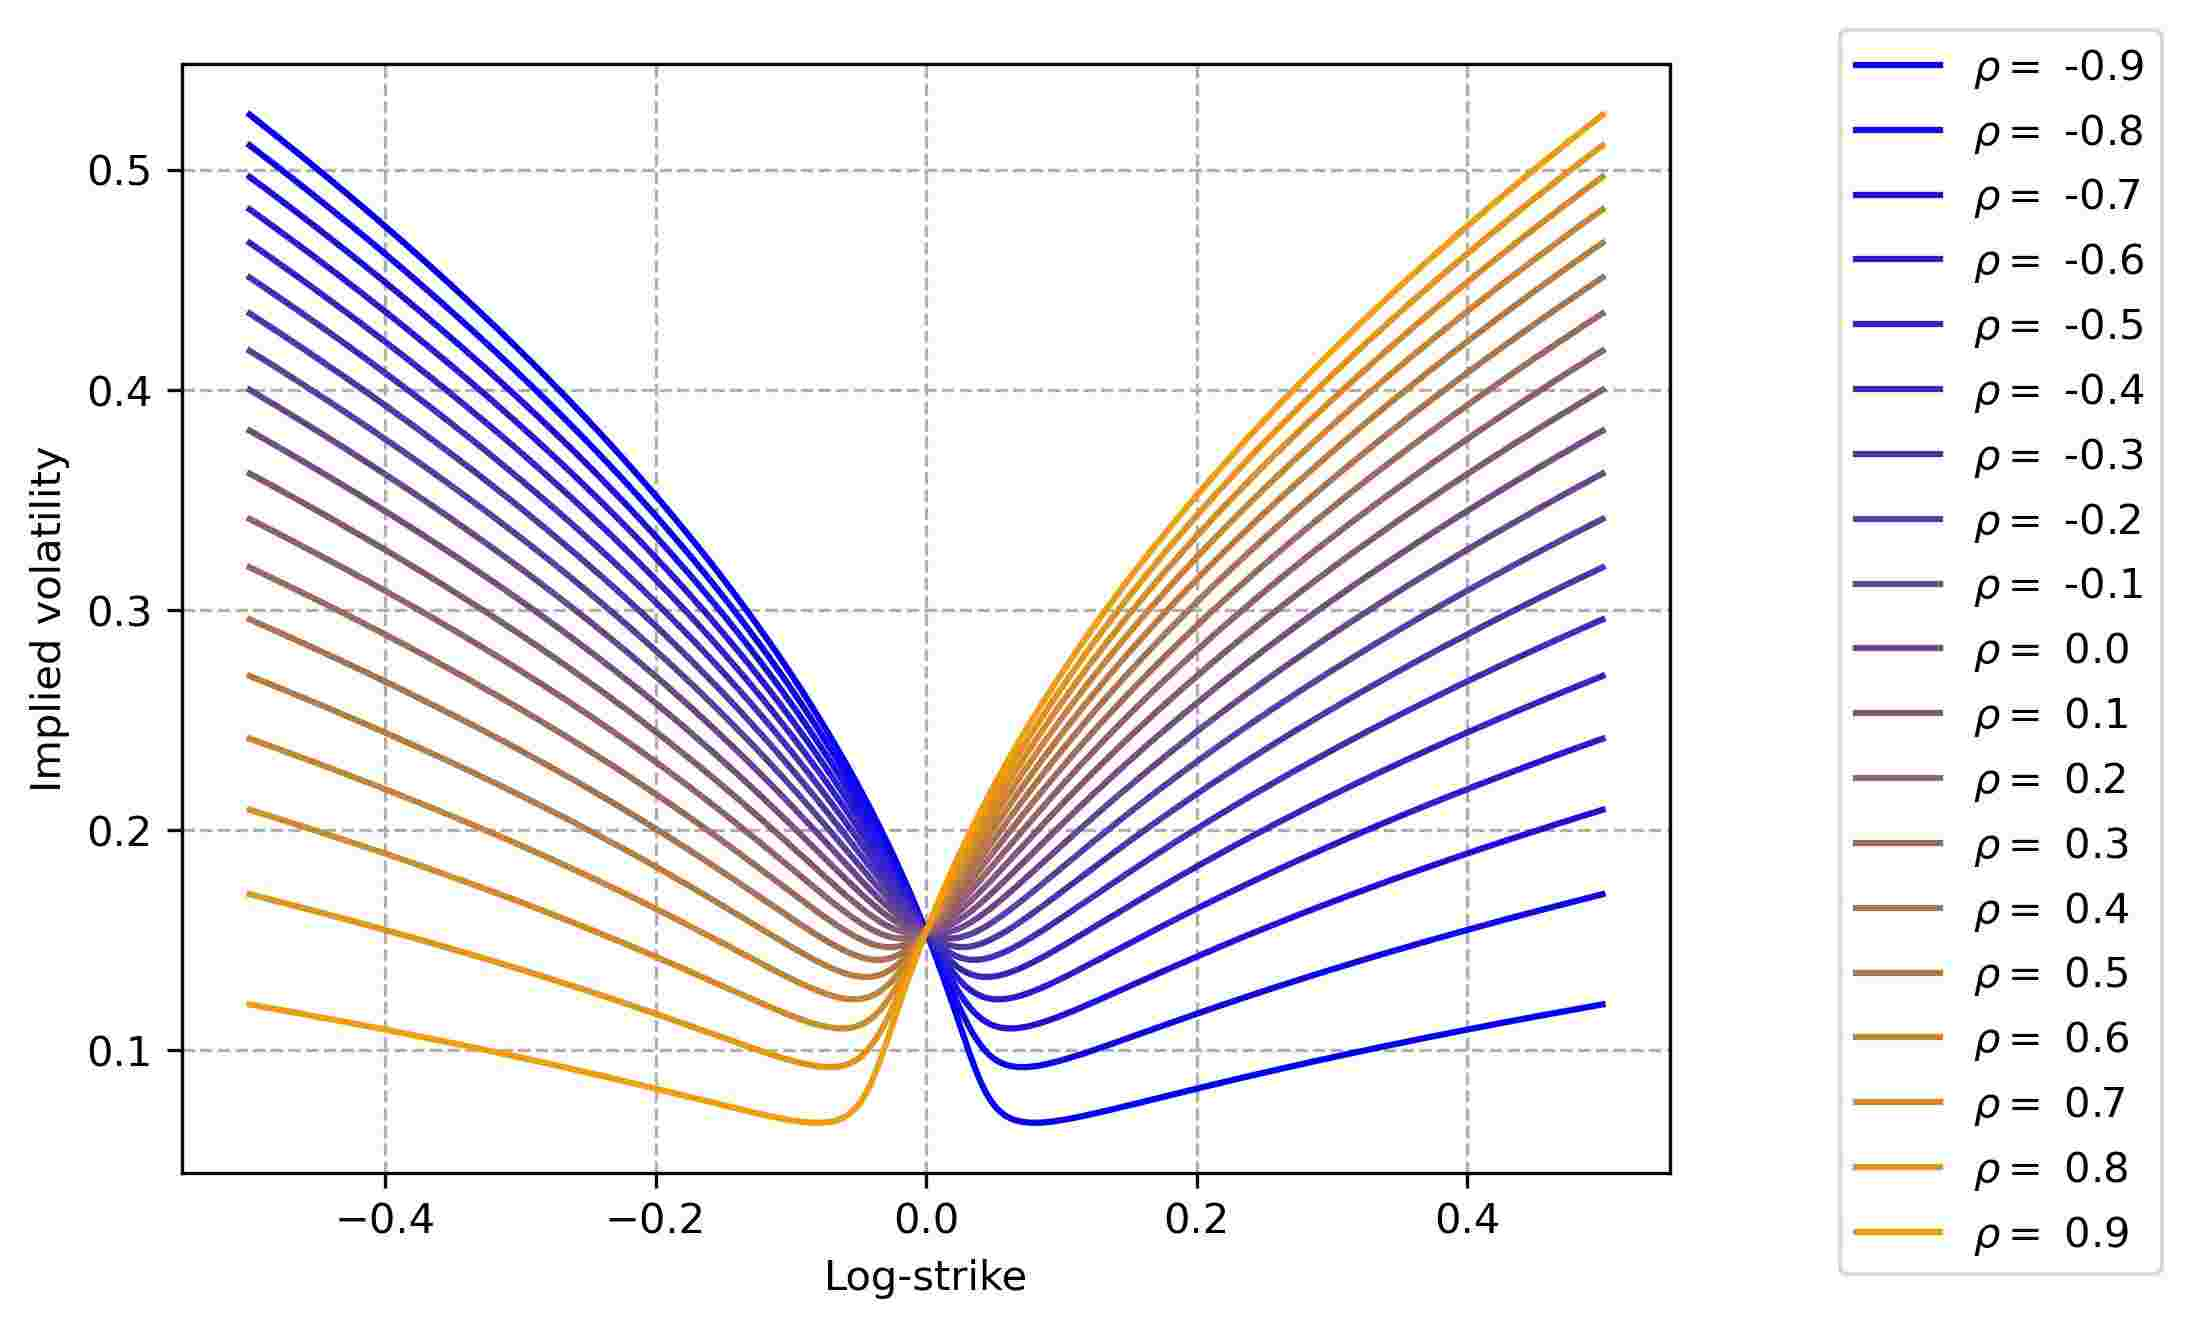
\includegraphics[width=0.45\linewidth]{influence_rho.jpg}}
    \subfigure[Influence of $\eta$]{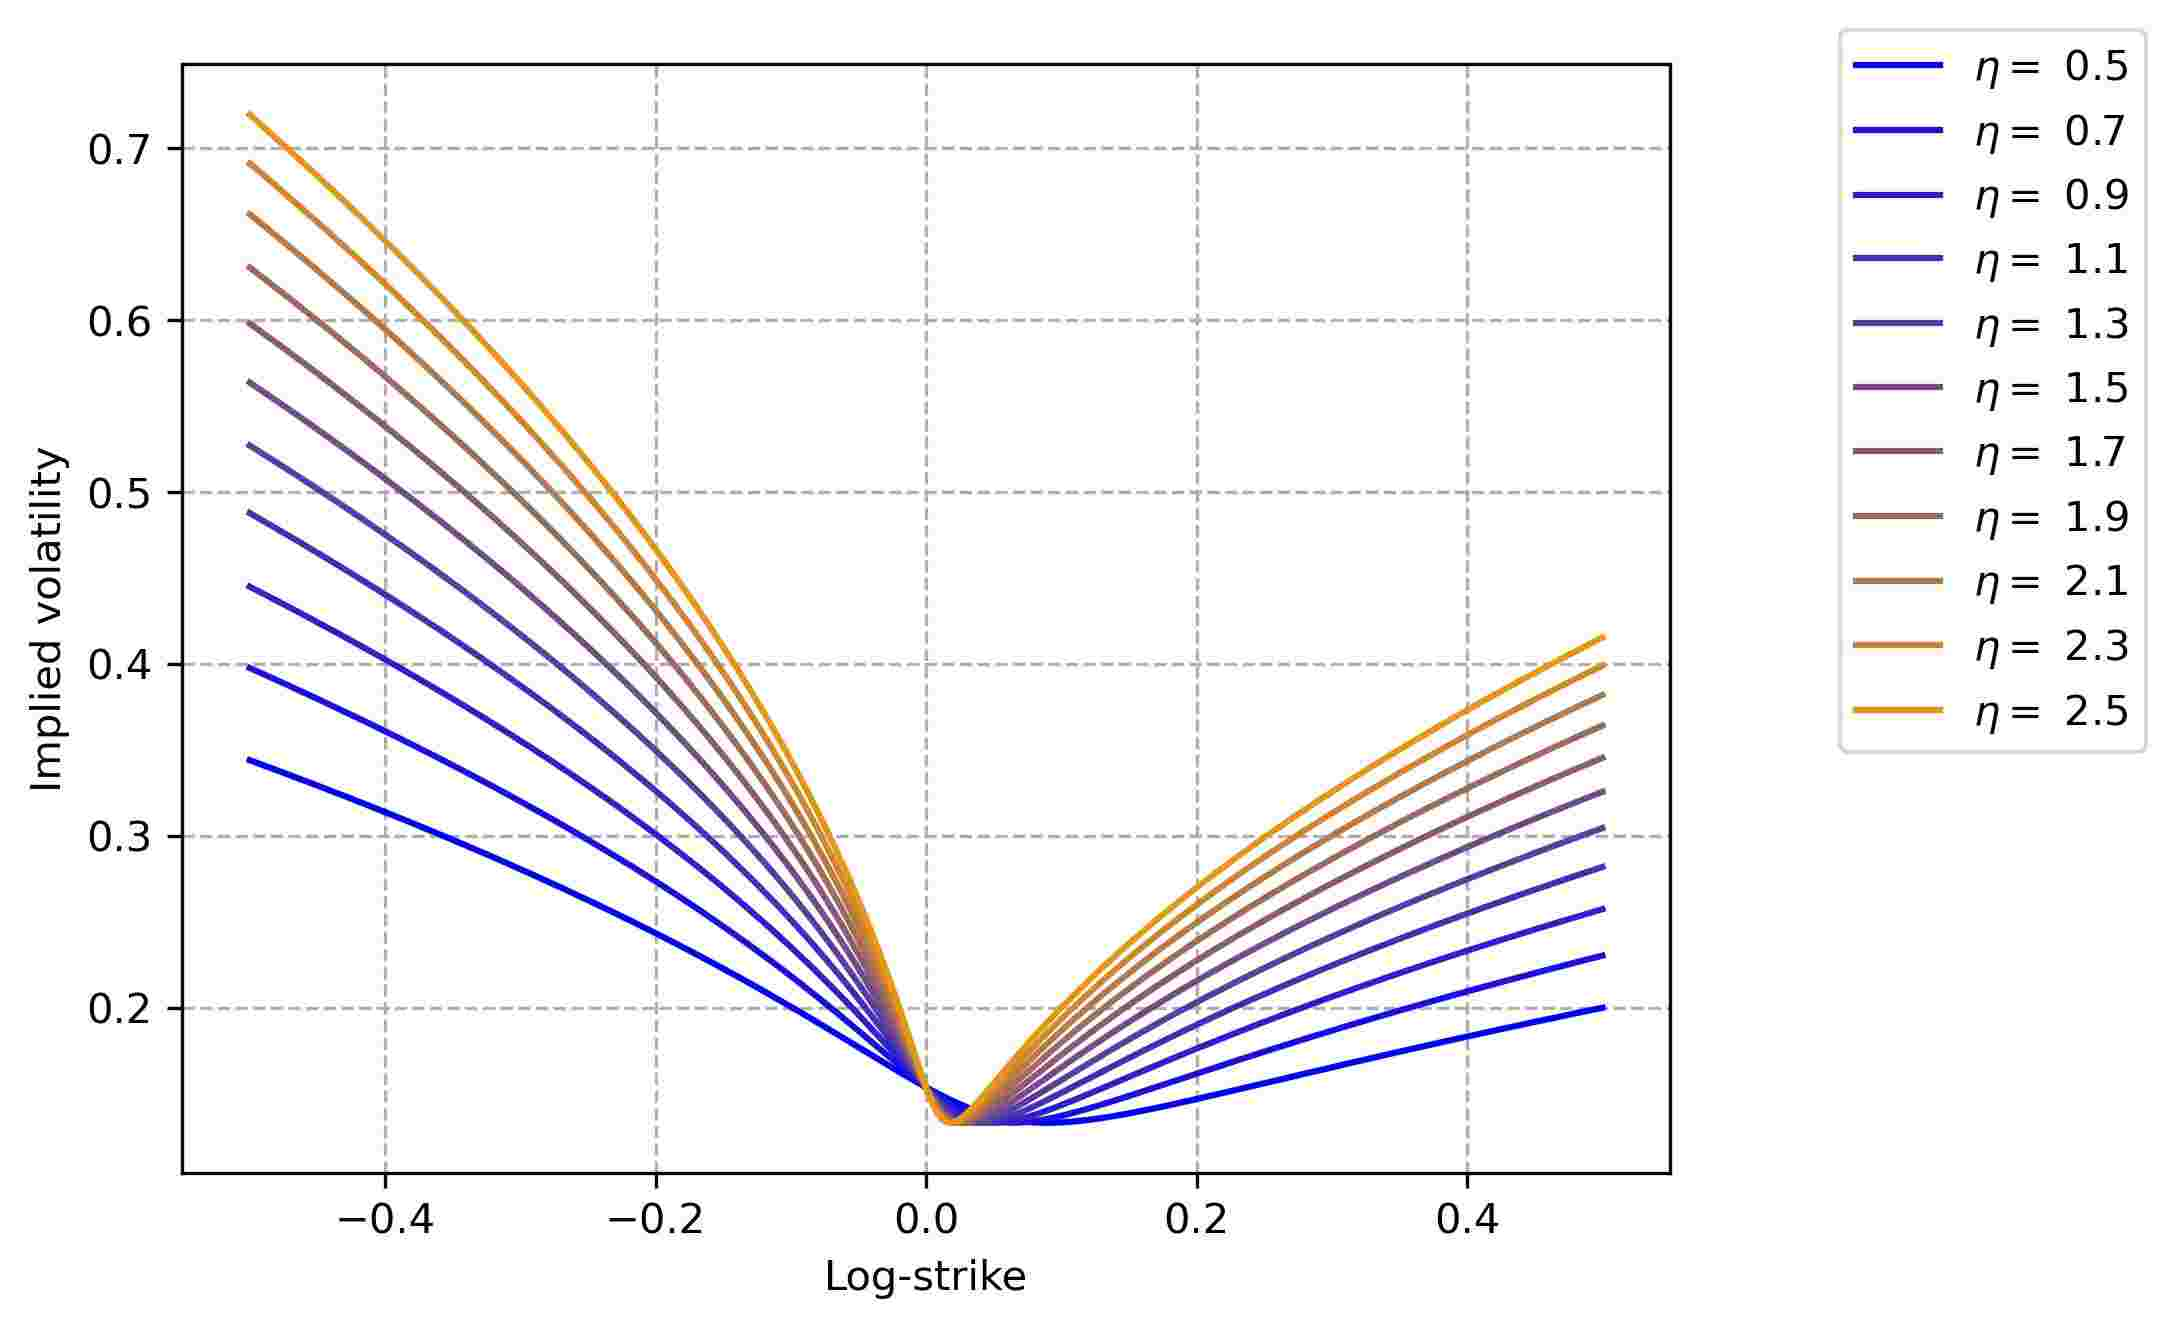
\includegraphics[width=0.45\linewidth]{influence_eta.jpg}}
    \caption{Influence of the $\rho$ and $\eta$ parameters on the shape of the implied volatility smile computed from the parsimonious SSVI ($a$ and $p$ are respectively fixed to 0.05 and 1.3).}
    \label{fig:influence_rho_eta}
\end{figure}


\subsection{Specification of the model for the underlying asset price and the IVS}\label{sec:dynamics_specification}
\subsubsection{Dynamics of the underlying asset price}
Based on the analysis in the previous section, we provide here the dynamics of the four parameters in the parsimonious SSVI model. Since two of these parameters depend on the past path of the underlying asset price, we also need a model for the dynamics of the underlying asset price in order to be able to simulate IVSs over time. Because we want these simulations to be realistic, the model for the underlying asset price should also be as realistic as possible. We opt for the PDV model by Guyon and Lekeufack (more precisely, a variant of their model as we will see) as it allows to replicate almost all historical stylized facts of equity prices (leverage effect, volatility clustering, weak and strong Zumbach effects). The asset price $(S_t)_{t\ge 0}$ is assumed to evolve as follows:
\begin{equation}\label{eq:underlying_dynamics}
    \left\{ 
    \begin{array}{rcl}
        \displaystyle\frac{dS_t}{S_t} &=& \mu_Sdt + \sigma_t dW^S_t \\
        \sigma_t &=&  \beta_0^{\sigma} + \beta_1^{\sigma} R^{\sigma}_{1,t}+\beta_2^{\sigma} \Sigma_t^{\sigma} \\
        R_{1,t}^{\sigma} &=& \displaystyle\int_{-\infty}^t \frac{Z_{\alpha_1^{\sigma},\delta_1^{\sigma}}}{(t-u+\delta_1^{\sigma})^{\alpha_1^{\sigma}}}\times \frac{dS_u}{S_u} \\
        \Sigma_t^{\sigma} &=& \sqrt{\displaystyle\int_{-\infty}^t \frac{Z_{\alpha_2^{\sigma},\delta_2^{\sigma}}}{(t-u+\delta_2^{\sigma})^{\alpha_2^{\sigma}}}\times\left(\frac{dS_u}{S_u}\right)^2}
    \end{array}
    \right.
\end{equation}
where $\mu_S$ is the drift, $\sigma_t$ is the instantaneous or spot volatility, $(W^S_t)_{t\ge 0}$ is a Brownian motion and $Z_{\alpha,\delta} = \left(\int_{-\infty}^t \frac{du}{(t-u+\delta)^{\alpha}} \right)^{-1}$. This specification is mostly similar to the one proposed by \cite{guyon2022volatility} but there are several differences. First, we do not approximate the TSPL kernels by linear combinations of exponential kernels. Guyon and Lekeufack make this approximation to recover a Markovian model that is very fast to simulate. We choose not to follow suit since we already achieve reasonable simulation times as we will show in the numerical experiments. Second, Guyon and Lekeufack propose to introduce multiplicative residuals in order to capture the exogenous part of the volatility, i.e. they specify the dynamics of the spot volatility as $\sigma_t = \kappa_t(\beta_0^{\sigma} + \beta_1^{\sigma} R^{\sigma}_{1,t}+\beta_2^{\sigma} \Sigma_t^{\sigma})$ where $(\kappa_t)_{t\ge 0}$ is an Ornstein-Uhlenbeck process or the exponential of an Ornstein-Uhlenbeck process. Again, we propose not to follow suit. Indeed, the estimation of the residuals requires to have realized volatility estimates in order to calibrate the PDV model. But when we use such estimates in the calibration, the log-returns simulated by the calibrated model are not as volatile as the historical log-returns. To be more precise, we implemented the following steps.
\begin{enumerate}
    \item We calibrate the PDV model on S\&P 500 realized volatility estimates (we use those of \citeauthor{heber2009oxford}, \citeyear{heber2009oxford} from 2000 to 2020) using the approach described in Section \ref{sec:calib_meth}.
    \item We calibrate an exponential Ornstein-Uhlenbeck process on the residuals $\kappa_t$ obtained as the ratio of the realized volatility estimates and the predicted volatilities.
    \item We simulate 1000 paths of the asset price $S$ over 3 years with a daily time step according to (\ref{eq:underlying_dynamics}) with the calibrated parameters.
\end{enumerate}
In this setting, the (annualized) standard deviation of the simulated log-returns is 13.2\% while the one of the historical log-returns is 19.9\% (estimated on the S\&P 500 daily log-returns from 2000 to 2020). Note that a similar discrepancy is observed if one considers additive residuals instead of multiplicative residuals. There are two reasons that can explain this discrepancy.
\begin{enumerate}
    \item We observe that when we filter the Brownian increments from the log-returns $\log \frac{S_{t_{i+1}}}{S_{t_i}}$ and the realized volatility estimates $\hat{\sigma}$ as:
    \begin{equation*}
        \hat{W}_{t_{i+1}}-\hat{W}_{t_i} =\frac{1}{\hat{\sigma}_{t_i}} \left( \log \frac{S_{t_{i+1}}}{S_{t_i}}+ \frac{1}{2}\hat{\sigma}_{t_i}^2(t_{i+1}-t_i) \right),
    \end{equation*}
    the tails of the obtained increments are fatter than those of a normal distribution (fitting a Student distribution on these increments actually yield a degree of freedom around 3). 
    \item The distribution of the log-returns does not appear in the target functions that are used in the above-mentioned calibration procedure so there are \textit{a priori} no reason that it will be reproduced by the calibrated model. 
\end{enumerate}
To remedy this problem, we propose to calibrate the parameters of the PDV model by log-likelihood maximization of the log-returns without using any realized volatility data and without considering any residuals in the PDV model. This calibration procedure will be described in more details in Section \ref{sec:model_calibration}. With this calibration procedure, the standard deviation of the simulated log-returns is 18.7\% so slightly below the historical one. The third and last difference with the model of \cite{guyon2022volatility} is the introduction of a drift in the dynamics of the asset price. This is first motivated by the fact that the S\&P 500 and the Euro Stoxx 50 have both significantly rised on the train set: the average annual log-return on the train set (i.e. between March 8, 2012 and December 31, 2020) is 11.5\% for the S\&P 500 and 3.9\% for the Euro Stoxx 50 so it is difficult to achieve a good fit to the data without adding a drift. Besides, we observed that without incorporating a drift, the model was unable to produce persistent periods of low volatility historically observed (for example from 2017 to 2018 for the S\&P 500, see Figure \ref{fig:data_sets}) which resulted in a simulated implied volatility that was, on average, higher than the historical one. When a positive drift is added\footnote{In practice, the calibrated drift $\mu_S$ is positive for both the S\&P 500 and the Euro Stoxx 50.}, the feature $R_1$ is indeed more likely to take positive values which is then reducing the volatility given that $\beta_1^{\sigma}<0$. As a consequence of this drift, the asset price is not a martingale. However, this is not an issue here as we are working under the real-world probability measure instead of a risk-neutral one. 

\begin{remark}
    As already mentioned in the introduction, for now, there does not exist conditions guaranteeing that the volatility $\sigma$ is positive in the PDV model when the two kernels are of the TSPL kind. However, with the calibrated parameters (see Section \ref{sec:model_calibration}), we did not observe any negative value in our simulations. 
\end{remark}


\subsubsection{Dynamics of the parsimonious SSVI parameters}
Since both parameters $a$ and $p$ in the parsimonious SSVI model exhibit a path-dependent behavior with respect to the underlying asset price, we propose the following dynamics for these parameters:
\begin{equation}\label{eq:a_p_dynamics}
    \left\{ 
    \begin{array}{rcll}
        a_t &=& \left|\beta_0^a+\beta_1^aR_{1,t}^a+(\beta_2^a+\varepsilon_t^a)\Sigma_t^a \right| \\
        p_t &=& \exp\left(\beta_0^p+\beta_1^pR_{1,t}^p+(\beta_2^p+\varepsilon_t^p)\Sigma_t^p\right) \\
        R_{1,t}^{i} &=& \displaystyle\int_{-\infty}^t \frac{Z_{\alpha_1^i,\delta_1^i}}{(t-u+\delta_1^i)^{\alpha_1^i}}\times \frac{dS_u}{S_u} & \text{for } i \in \{a,p\}\\
        \Sigma_t^{i} &=& \sqrt{\displaystyle\int_{-\infty}^t \frac{Z_{\alpha_2^i,\delta_2^i}}{(t-u+\delta_2^i)^{\alpha_2^i}}\times\left(\frac{dS_u}{S_u}\right)^2} & \text{for } i \in \{a,p\}
    \end{array}
    \right.
\end{equation}
where $\varepsilon^a$ and $\varepsilon^p$ are time-dependent residuals allowing to capture the variations in $a$ and $p$ that are not due to the past movements in the underlying asset price. Note that we consider that the residuals $\varepsilon^a$ and $\varepsilon^p$ are both multiplying the volatility feature of the PDV model instead of being purely additive terms of the linear regressions. Such a specification allows taking into account the fact that we observe historically larger deviations
of $\beta_0^a+\beta_1^aR_{1,t}^a+\beta_2^a\Sigma_t^a$ (resp. $\beta_0^p+\beta_1^pR_{1,t}^p+\beta_2^p\Sigma_t^p$) from $a_t$ (resp. $\log p_t$) when the volatility feature $\Sigma_t^a$ (resp. $\Sigma_t^p$) is large. Given the high autocorrelation of these residuals, we model both of them as centered Ornstein-Uhlenbeck processes:
\begin{equation}\label{eq:ou_processes}
    d\varepsilon_t^i = -\kappa_i\varepsilon_t^i dt + \gamma_i dW_t^i, \quad i\in \{a,p\}. 
\end{equation}
where $W^a$ and $W^p$ are two correlated Brownian motions that are also correlated to the Brownian motion $W^S$ driving the asset price. 

\begin{remark}
    Note that we consider different TSPL kernels parameters for $\sigma$, $a$ and $p$. Choosing to have common features $R_1$ and $\Sigma$ for $\sigma$, $a$ and $p$ with parameter-specific $\beta$'s is also an option but it requires to simultaneously calibrate the PDV model on the three time series and it would probably reduce the $R^2$ scores in comparison to the ones obtained with a calibration of the PDV model for each of the three variables. \\
\end{remark}

\begin{remark}
    The above specification guarantees that both $a$ and $p$ are always positive. Since the ATM total variance is parameterized as $\theta_T=aT^p$, it implies that $\partial_T \theta_T\ge 0$ so that there is no calendar arbitrage (see Appendix \ref{sec:ssvi_arbitrage}). In our simulations, we observe that $\beta_0^a+\beta_1^a+(\beta_2^a+\varepsilon^a_t)\Sigma_t^a$ is actually always positive so the absolute value is not necessary. 
\end{remark}

The two remaining parameters of the parsimonious SSVI model, namely $\rho$ and $\eta$, are more difficult to predict using the past returns and past squared returns (see Section \ref{sec:pdv_ssvi_params}). Thus, we do not rely on a PDV model to describe their dynamics. We propose to model both parameters as Jacobi processes guaranteeing that $\rho \in [-1,1]$ and $\eta\in [0,\sqrt{2}]$:
\begin{equation}\label{eq:jacobi_processes}
    \left\{
    \begin{array}{rcl}
        d\rho_t &=& \kappa_{\rho}(\mu_\rho -\rho_t)dt  +\gamma_{\rho}\sqrt{(1-\rho_t)(1+\rho_t)} dW_t^{\rho}, \\
        d\eta_t &=& \kappa_{\eta}(\mu_{\eta} - \eta_t)dt +\gamma_{\eta}\sqrt{(\sqrt{2}-\eta_t)\eta_t} dW_t^{\eta}, \\
    \end{array}
    \right.
\end{equation}
where $\kappa_\rho,\kappa_{\eta}>0$, $\mu_{\rho}\in [-1,1]$, $\mu_{\eta}\in[0,\sqrt{2}]$, $\gamma_{\rho},\gamma_{\eta}>0$, $W^{\rho}$ and $W^{\eta}$ are two correlated Brownian motions that are also correlated to $W^S$, $W^a$ and $W^p$. This modelling choice is motivated by two reasons. First, both parameters are highly autocorrelated. Second, we recall that the parsimonious SSVI model is free of static arbitrage provided that $\eta^2(1+|\rho|) \le 4$. A sufficient condition for this condition to be satisfied is therefore: $\rho \in [-1,1]$ (which is anyway the domain of definition of $\rho$) and $\eta \in [0,\sqrt{2}]$. It turns out that this condition is always satisfied by the calibrated $\rho$ and $\eta$. Hence, by using the Jacobi processes as specified above, we make sure that the simulated implied volatility surfaces are free from static arbitrage. 


\begin{remark}
    The model obtained by combining Equations (\ref{eq:underlying_dynamics}), (\ref{eq:a_p_dynamics}), (\ref{eq:ou_processes}) and (\ref{eq:jacobi_processes}) is called the path-dependent SSVI model. 
\end{remark}


\subsection{Model calibration}\label{sec:model_calibration}
This section details a calibration methodology for all the parameters involved in the path-dependent SSVI model whose dynamics has been specified in the previous section. \\

We discretize the asset price along a time grid $(t_k)_{k\ge 0}$ by the specifying the log-returns $r_{t_{k+1}}=\log \frac{S_{t_{k+1}}}{S_{t_k}}$ as:
\begin{equation*}
    r_{t_{k+1}} = \left(\mu_S-\frac{\sigma_{t_k}^2}{2}\right)(t_{k+1}-t_k) + \sigma_{t_k} \sqrt{t_{k+1}-t_k} \varepsilon_{t_{k+1}}^S
\end{equation*}
where $\sigma_{t_k} = \beta_0^{\sigma}+\beta_1^{\sigma}R_{1,t_k}^{\sigma}+\beta_2^{\sigma}\Sigma_{t_k}^{\sigma}$ and $(\varepsilon^S_{t_k})_{1\le k \le N}$ are i.i.d. standard normal random variables. The features $R_1^{\sigma}$ and $\Sigma^{\sigma}$ are discretized and truncated as:
\begin{equation*}
    R_{1,t} = \sum_{t-C_{R_1}^{\sigma}\le t_k \le t} \frac{Z_{\alpha_1^{\sigma},\delta_1^{\sigma}}}{(t-t_k+\delta_1^{\sigma})^{\alpha_1^{\sigma}}} r_{t_k} \text{ and } \Sigma_{t} = \sqrt{\sum_{t-C_{\Sigma}^{\sigma}\le t_k \le t} \frac{Z_{\alpha_2^{\sigma},\delta_2^{\sigma}}}{(t-t_k+\delta_2^{\sigma})^{\alpha_2^{\sigma}}} r_{t_k}^2}.
\end{equation*}
The parameters $(\mu_S,\alpha_1^{\sigma},\delta_1^{\sigma},\alpha_2^{\sigma},\delta_2^{\sigma},\beta_0^{\sigma},\beta_1^{\sigma},\beta_2^{\sigma})$ are estimated by log-likelihood maximization of the log-returns. Indeed, with the above discretizations, the distribution of $r_{t_{k+1}}$ conditionally on all the information available at time $t_k$ is a normal distribution with mean $ \left(\mu_S-\frac{\sigma_{t_k}^2}{2}\right)(t_{k+1}-t_k)$ and variance $\sigma_{t_k}^2 (t_{k+1}-t_k)$. Thus, it is possible to write explicitly the log-likelihood of the vector of observed log-returns $(r^h_{t_1},\dots,r^h_{t_N})$ as a function of the drift and the 7 PDV parameters and to maximize it using a numerical optimization routine. The cut-off lags $C_{R_1}^{\sigma}$ and $C_{\Sigma}^{\sigma}$ are estimated on the realized volatility estimates from \cite{heber2009oxford} using the approach described in Appendix \ref{sec:influence_cutoff}.\\

The calibration methodology of the PDV parameters $\alpha_1^i$, $\delta_1^i$, $\alpha_2^i$, $\delta_2^i$, $\beta_0^i$, $\beta_1^i$ and $\beta_2^i$ for $i\in \{a,p\}$ in Equation (\ref{eq:a_p_dynamics}) is the same as the one exposed in Section \ref{sec:calib_meth}. The cut-off lags $C_{R_1}^i$ and $C_{\Sigma}^i$ are those presented in Appendix \ref{sec:hyperparams_ssvi}. We deduce the historical time series of $\varepsilon^a$ and $\varepsilon^p$ from this calibration. The parameters $\kappa_i$ and $\gamma_i$ of the Ornstein-Uhlenbeck processes in Equation (\ref{eq:ou_processes}) are then calibrated on these time series using the maximum likelihood estimators from \cite{tang2009parameter}. The parameters $\kappa_i$, $\mu_i$ and $\gamma_i$ for $i\in\{\rho,\eta\}$ are calibrated using the following estimators\footnote{Note that these estimators generalize the ones developed by \cite{wei2016} in the case of the CIR process. } which are obtained by maximizing the log-likelihood of a Jacobi process discretized using the Euler-Maruyama scheme: 
\begin{equation*}
    \begin{array}{rcl}
        \hat{\kappa}_i &=& \displaystyle\frac{1}{\Delta} \times \frac{
             \displaystyle\sum_{k=0}^{N-1} \frac{x^i_{t_{k+1}} - x^i_{t_k}}{Q_i\left(x^i_{t_k}\right)} 
             \displaystyle\sum_{k=0}^{N-1} \frac{x^i_{t_k}}{Q_i\left(x^i_{t_k}\right)}  
            - \displaystyle\sum_{k=0}^{N-1} \frac{(x^i_{t_{k+1}} - x^i_{t_k}) x^i_{t_k}}{Q_i\left(x^i_{t_k}\right)}
            \displaystyle\sum_{k=0}^{N-1} \frac{1}{Q_i\left(x^i_{t_k}\right)} 
            }{
            \displaystyle\sum_{k=0}^{N-1} \frac{1}{Q_i\left(x^i_{t_k}\right)}  
             \displaystyle\sum_{k=0}^{N-1} \frac{\left(x^i_{t_k}\right)^2}{Q_i\left(x^i_{t_k}\right)} 
            - \left( \displaystyle\sum_{k=0}^{N-1} \frac{x^i_{t_k}}{Q_i\left(x^i_{t_k}\right)} \right)^2
            },\\
    \hat{\mu}_i &=& \displaystyle\frac{1}{\hat{\kappa}_i\Delta} \times \frac{\displaystyle\sum_{k=0}^{N-1}\frac{x^i_{t_{k+1}}-x^i_{t_k}+\hat{\kappa}_i x^i_{t_k}\Delta}{Q_i\left(x^i_{t_k}\right)}}{\displaystyle\sum_{k=0}^{N-1}\frac{1}{Q_i\left(x^i_{t_k}\right)}}, \\
    \hat{\gamma}_i &=& \displaystyle\frac{1}{N\Delta} \displaystyle\sum_{k=0}^{N-1} \frac{
        \left( x^i_{t_{k+1}} - x^i_{t_k} - \hat{\kappa}_i \left( \hat{\mu}_i - x^i_{t_k} \right) \Delta \right)^2
        }{Q_i\left( x^i_{t_k} \right)}
    \end{array}
\end{equation*}
where $i\in\{\rho,\eta \}$, $(x^i_{t_k})_{k=0,\dots,N}$ are the historical observations of $i$, $Q_{\rho}(x)=(1-x)(1+x)$, $Q_{\eta}(x)=x(\sqrt{2}-x)$ and $\Delta$ is the time step of the grid $(t_k)_{k=0,\dots,N}$ which is assumed to be constant from now on. Finally, once all the above parameters are calibrated, the correlations between the Brownian motions $W^S$, $W^a$, $W^p$, $W^{\rho}$ and $W^{\eta}$ are set to the empirical correlations between the residuals $\hat{\varepsilon}^S$, $\hat{\nu}^a$, $\hat{\nu}^p$, $\hat{\varepsilon}^{\rho}$, $\hat{\varepsilon}^{\eta}$ of the models for $S$, $\varepsilon^a$, $\varepsilon^p$, $\rho$ and $\eta$ respectively. These residuals are computed as:
\begin{equation*}
    \begin{array}{rcll}
        \hat{\varepsilon}^S_{t_{k+1}} &=& \displaystyle\frac{r^h_{t_{k+1}}-\left(\hat{\mu}_S-\frac{\sigma_{t_k}^2}{2}\right)\Delta}{\sigma_{t_k}\sqrt{\Delta}}, \\
        \hat{\nu}^i_{t_{k+1}} &=& \displaystyle\frac{\hat{\varepsilon}^i_{t_{k+1}}-\hat{\varepsilon}^i_{t_{k}}e^{-\hat{\kappa}_i\Delta}}{\hat{\gamma}_i\sqrt{\frac{1-e^{-2\hat{\kappa}_i\Delta}}{2\hat{\kappa}_i}}},& \text{for } i \in \{a,p\}, \\
        \hat{\varepsilon}^x_{t_{k+1}} &=& \displaystyle \frac{x_{t_{k+1}}-x_{t_k}-\hat{\kappa}_x(\hat{\mu}_x-x_{t_k})\Delta}{\hat{\gamma}_x\sqrt{\Delta Q_x(x_{t_k})}}, & \text{for } x \in \{\rho,\eta\},  
    \end{array}
\end{equation*}
where the $\hat{q}$ denotes the estimated value of the parameter $q$. In Table \ref{tab:sp500_params} and \ref{tab:sx5e_params}, we report the calibrated parameters for the S\&P 500 and the Euro Stoxx 50 data sets. The calibration period is the same as the one used for the training of the PDV model in Section \ref{sec:empirical_study}, namely from March 8, 2012 to December 31, 2020. 


\begin{table}[htbp]
    \centering
    \caption{Calibrated parameters of the path-dependent SSVI model on the S\&P 500 data set. }
    \label{tab:sp500_params}
    \begin{tabular}{@{}lllllllll@{}}
    \toprule
    \multicolumn{1}{c}{\multirow{2}{*}{$S$}} & $\alpha_1^{\sigma}$ & $\delta_1^{\sigma}$ & $\alpha_2^{\sigma}$ & $\delta_2^{\sigma}$ & $\beta_0^{\sigma}$ & $\beta_1^{\sigma}$ &  $\beta_2^{\sigma}$& $\mu_S$ \\ \cmidrule(l){2-9} 
    \multicolumn{1}{c}{}                   &7.74  & 0.12 & 2.42 & 0.06 & 0.03 & -0.04 & 0.84 & 0.07 \\ \cmidrule(r){1-9}
    \multicolumn{1}{c}{\multirow{2}{*}{$a$}} & $\alpha_1^{a}$ & $\delta_1^{a}$ & $\alpha_2^{a}$ & $\delta_2^{a}$ & $\beta_0^{a}$ & $\beta_1^{a}$ &  $\beta_2^{a}$ \\ \cmidrule(l){2-8} 
    \multicolumn{1}{c}{}                   &1.12  & 0.03 & 0.88 & 0.03 & -8.71$\times 10^{-4}$ & -0.02 & 0.22 \\ \cmidrule(r){1-9}
    \multicolumn{1}{c}{\multirow{2}{*}{$p$}} & $\alpha_1^{p}$ & $\delta_1^{p}$ & $\alpha_2^{p}$ & $\delta_2^{p}$ & $\beta_0^{p}$ & $\beta_1^{p}$ &  $\beta_2^{p}$ \\ \cmidrule(l){2-8} 
    \multicolumn{1}{c}{}                   &1.01  & 0.02 & 0.78 & 0.01 & 0.36 & 0.11 & -1.35 \\ \cmidrule(r){1-9}
    \multicolumn{1}{c}{\multirow{2}{*}{$\varepsilon^a$}} & $\kappa_a$ & $\gamma_a$  \\ \cmidrule(l){2-3} 
    \multicolumn{1}{c}{}                   &16.3  & 0.11  \\ \cmidrule(r){1-9} 
    \multicolumn{1}{c}{\multirow{2}{*}{$\varepsilon^p$}} & $\kappa_p$ & $\gamma_p$  \\ \cmidrule(l){2-3} 
    \multicolumn{1}{c}{}                   &26.4  & 3.24  \\ \cmidrule(r){1-9} 
    \multicolumn{1}{c}{\multirow{2}{*}{$\rho$}} & $\kappa_{\rho}$ & $\mu_{\rho}$ & $\gamma_{\rho}$  \\ \cmidrule(l){2-4} 
    \multicolumn{1}{c}{}                   &60.4  & -0.71 & 0.99  \\ \cmidrule(r){1-9} 
    \multicolumn{1}{c}{\multirow{2}{*}{$\eta$}} & $\kappa_{\eta}$ & $\mu_{\eta}$ & $\gamma_{\eta}$  \\ \cmidrule(l){2-4} 
    \multicolumn{1}{c}{}                   &8.86  & 0.93 & 0.62   \\ 
    \bottomrule
    \end{tabular}
    \end{table}

    
\begin{table}[htbp]
    \centering
    \caption{Calibrated parameters of the path-dependent SSVI model on the Euro Stoxx 50 data set. }
    \label{tab:sx5e_params}
    \begin{tabular}{@{}lllllllll@{}}
    \toprule
    \multicolumn{1}{c}{\multirow{2}{*}{$S$}} & $\alpha_1^{\sigma}$ & $\delta_1^{\sigma}$ & $\alpha_2^{\sigma}$ & $\delta_2^{\sigma}$ & $\beta_0^{\sigma}$ & $\beta_1^{\sigma}$ &  $\beta_2^{\sigma}$& $\mu_S$ \\ \cmidrule(l){2-9} 
    \multicolumn{1}{c}{}                   &2.01  & 0.03 & 2.01 & 0.05 & 0.04 & -0.04 & 0.80 & 0.06 \\ \cmidrule(r){1-9}
    \multicolumn{1}{c}{\multirow{2}{*}{$a$}} & $\alpha_1^{a}$ & $\delta_1^{a}$ & $\alpha_2^{a}$ & $\delta_2^{a}$ & $\beta_0^{a}$ & $\beta_1^{a}$ &  $\beta_2^{a}$ \\ \cmidrule(l){2-8} 
    \multicolumn{1}{c}{}                   &0.35  & 1.85$\times 10^{-3}$ & 1.04 & 0.07 & -0.01 & -2.67$\times 10^-3$ & 0.25 \\ \cmidrule(r){1-9}
    \multicolumn{1}{c}{\multirow{2}{*}{$p$}} & $\alpha_1^{p}$ & $\delta_1^{p}$ & $\alpha_2^{p}$ & $\delta_2^{p}$ & $\beta_0^{p}$ & $\beta_1^{p}$ &  $\beta_2^{p}$ \\ \cmidrule(l){2-8} 
    \multicolumn{1}{c}{}                   &0.57  & 0.01 & 0.99 & 0.01 & 0.25 & 0.27 & -1.05 \\ \cmidrule(r){1-9}
    \multicolumn{1}{c}{\multirow{2}{*}{$\varepsilon^a$}} & $\kappa_a$ & $\gamma_a$  \\ \cmidrule(l){2-3} 
    \multicolumn{1}{c}{}                   &12.1 & 0.10  \\ \cmidrule(r){1-9} 
    \multicolumn{1}{c}{\multirow{2}{*}{$\varepsilon^p$}} & $\kappa_p$ & $\gamma_p$  \\ \cmidrule(l){2-3} 
    \multicolumn{1}{c}{}                   &17.7  & 2.62  \\ \cmidrule(r){1-9} 
    \multicolumn{1}{c}{\multirow{2}{*}{$\rho$}} & $\kappa_{\rho}$ & $\mu_{\rho}$ & $\gamma_{\rho}$  \\ \cmidrule(l){2-4} 
    \multicolumn{1}{c}{}                   &12.7  & -0.56 & 0.31  \\ \cmidrule(r){1-9} 
    \multicolumn{1}{c}{\multirow{2}{*}{$\eta$}} & $\kappa_{\eta}$ & $\mu_{\eta}$ & $\gamma_{\eta}$  \\ \cmidrule(l){2-4} 
    \multicolumn{1}{c}{}                   &3.89  & 0.83 & 0.53  \\ 
    \bottomrule
    \end{tabular}
    \end{table}


\subsection{Numerical results}\label{sec:num_results}

The aim of this section is to provide some evidence of the consistency of the proposed model with historical underlying prices and IVSs data.  \\

\subsubsection{Simulation of the implied volatility surface conditionally on the historical path of the underlying asset price}\label{sec:cond_simus}
\begin{figure}[htbp]
    \centering
    \subfigure[Historical path of the S\&P 500 ATM term structure]{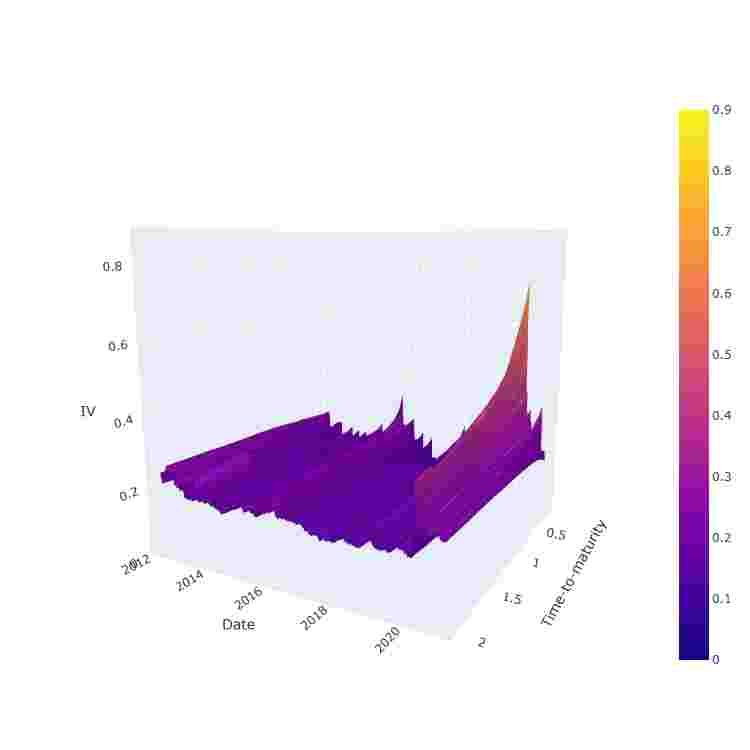
\includegraphics[width=0.45\linewidth]{SPX_ATM_Hist_IV.jpg}}
    \subfigure[Average path of the S\&P 500 ATM term structure]{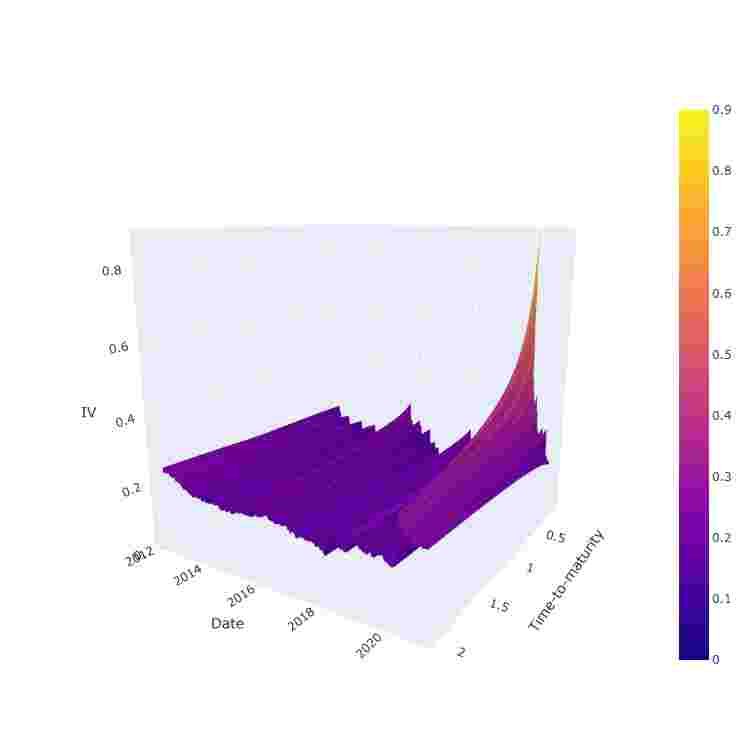
\includegraphics[width=0.45\linewidth]{SPX_ATM_Cond_Simu_IV.jpg}}
    \subfigure[Historical path of the Euro Stoxx 50 ATM term structure]{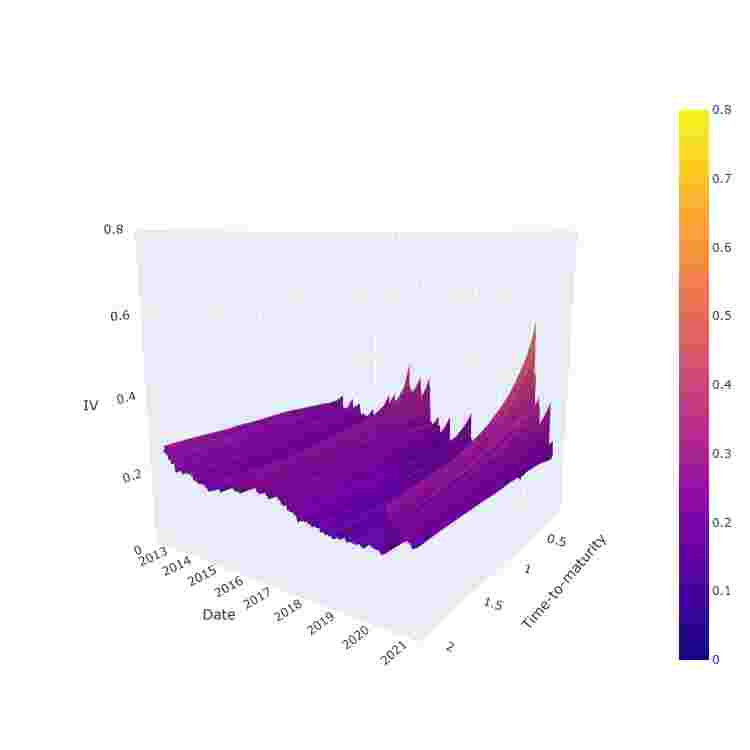
\includegraphics[width=0.45\linewidth]{SX5E_ATM_Hist_IV.jpg}}
    \subfigure[Average path of the Euro Stoxx 50 ATM term structure]{ 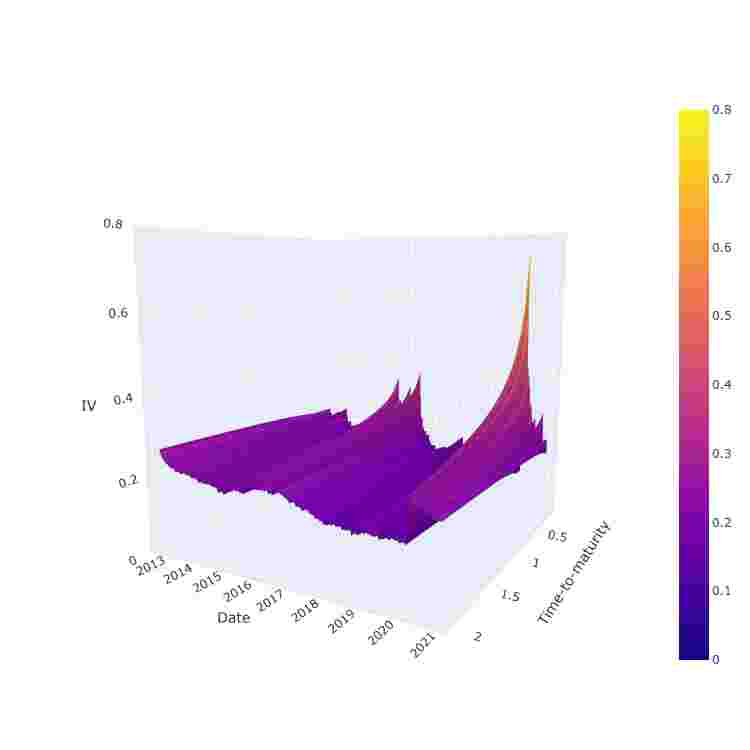
\includegraphics[width=0.45\linewidth]{SX5E_ATM_Cond_Simu_IV.jpg}}
    \caption{Comparison of the historical IVS ATM term structure to the average one simulated by the path-dependent SSVI model conditionally on the underlying historical path. }
\label{fig:cond_sample_paths}
\end{figure}
Using the calibrated parameters, we first simulate 1000 daily (i.e. the simulation time step is 1/252) trajectories of $(\varepsilon^a,\varepsilon^p,\eta,\rho)$ over 2185 days (the length of the train data sets) conditionally on the path of the S\&P 500 index between March 22, 2006 and December 31, 2020 and the path of the Euro Stoxx 50 index between September 26, 2006 and December 31, 2020 (the period from March 8, 2012 to December 31, 2020 corresponds to the one being used for the calibration of the path-dependent SSVI model and the period before is the one required for computing the features $R_1$ and $\Sigma$). The Ornstein-Uhlenbeck processes are simulated exactly while the Jacobi process is simulated using the full truncation Euler scheme of \cite{lord2010}. In Figure \ref{fig:cond_sample_paths}, we compare the historical time evolution of the ATM implied volatility curve as a function of the time-to-maturity (in the sequel, we refer to this curve as the IVS ATM term structure) to the one of the average path of the path-dependent SSVI model. We observe that the historical and the simulated paths are visually very close in terms of the level, the amplitude of the variations, the regularity and the overall shape. Moreover, the spikes of the implied volatility due to a drop in the underlying asset price (in particular in March 2020) are well reproduced. \\

Second, we simulate 1000 daily trajectories of $(\varepsilon^a,\varepsilon^p,\eta,\rho)$ over 2 years conditionally on the path of the S\&P 500 index between January 14, 2015 and December 31, 2022 and the path of the Euro Stoxx 50 index between February 25, 2015 and December 31, 2022. This second simulation batch allows an out-of-sample comparison while the first one allowed an in-sample comparison. In Figure \ref{fig:iv_prediction}, we demonstrate the out-of-sample predictive power of our model for 1-month, 12-month and 24-month ATM implied volatilities. The obtained $R^2$ scores are a bit smaller than those displayed in empirical study in Section \ref{sec:overall_perf} but let us emphasize here that it is not the ATM implied volatility for each time-to-maturity that is modelled using the PDV model but the parameters $a$ and $p$ of the parsimonious SSVI.

\begin{figure}[htbp]
    \centering
    \subfigure[1-month ATM implied volatility (S\&P 500)]{ 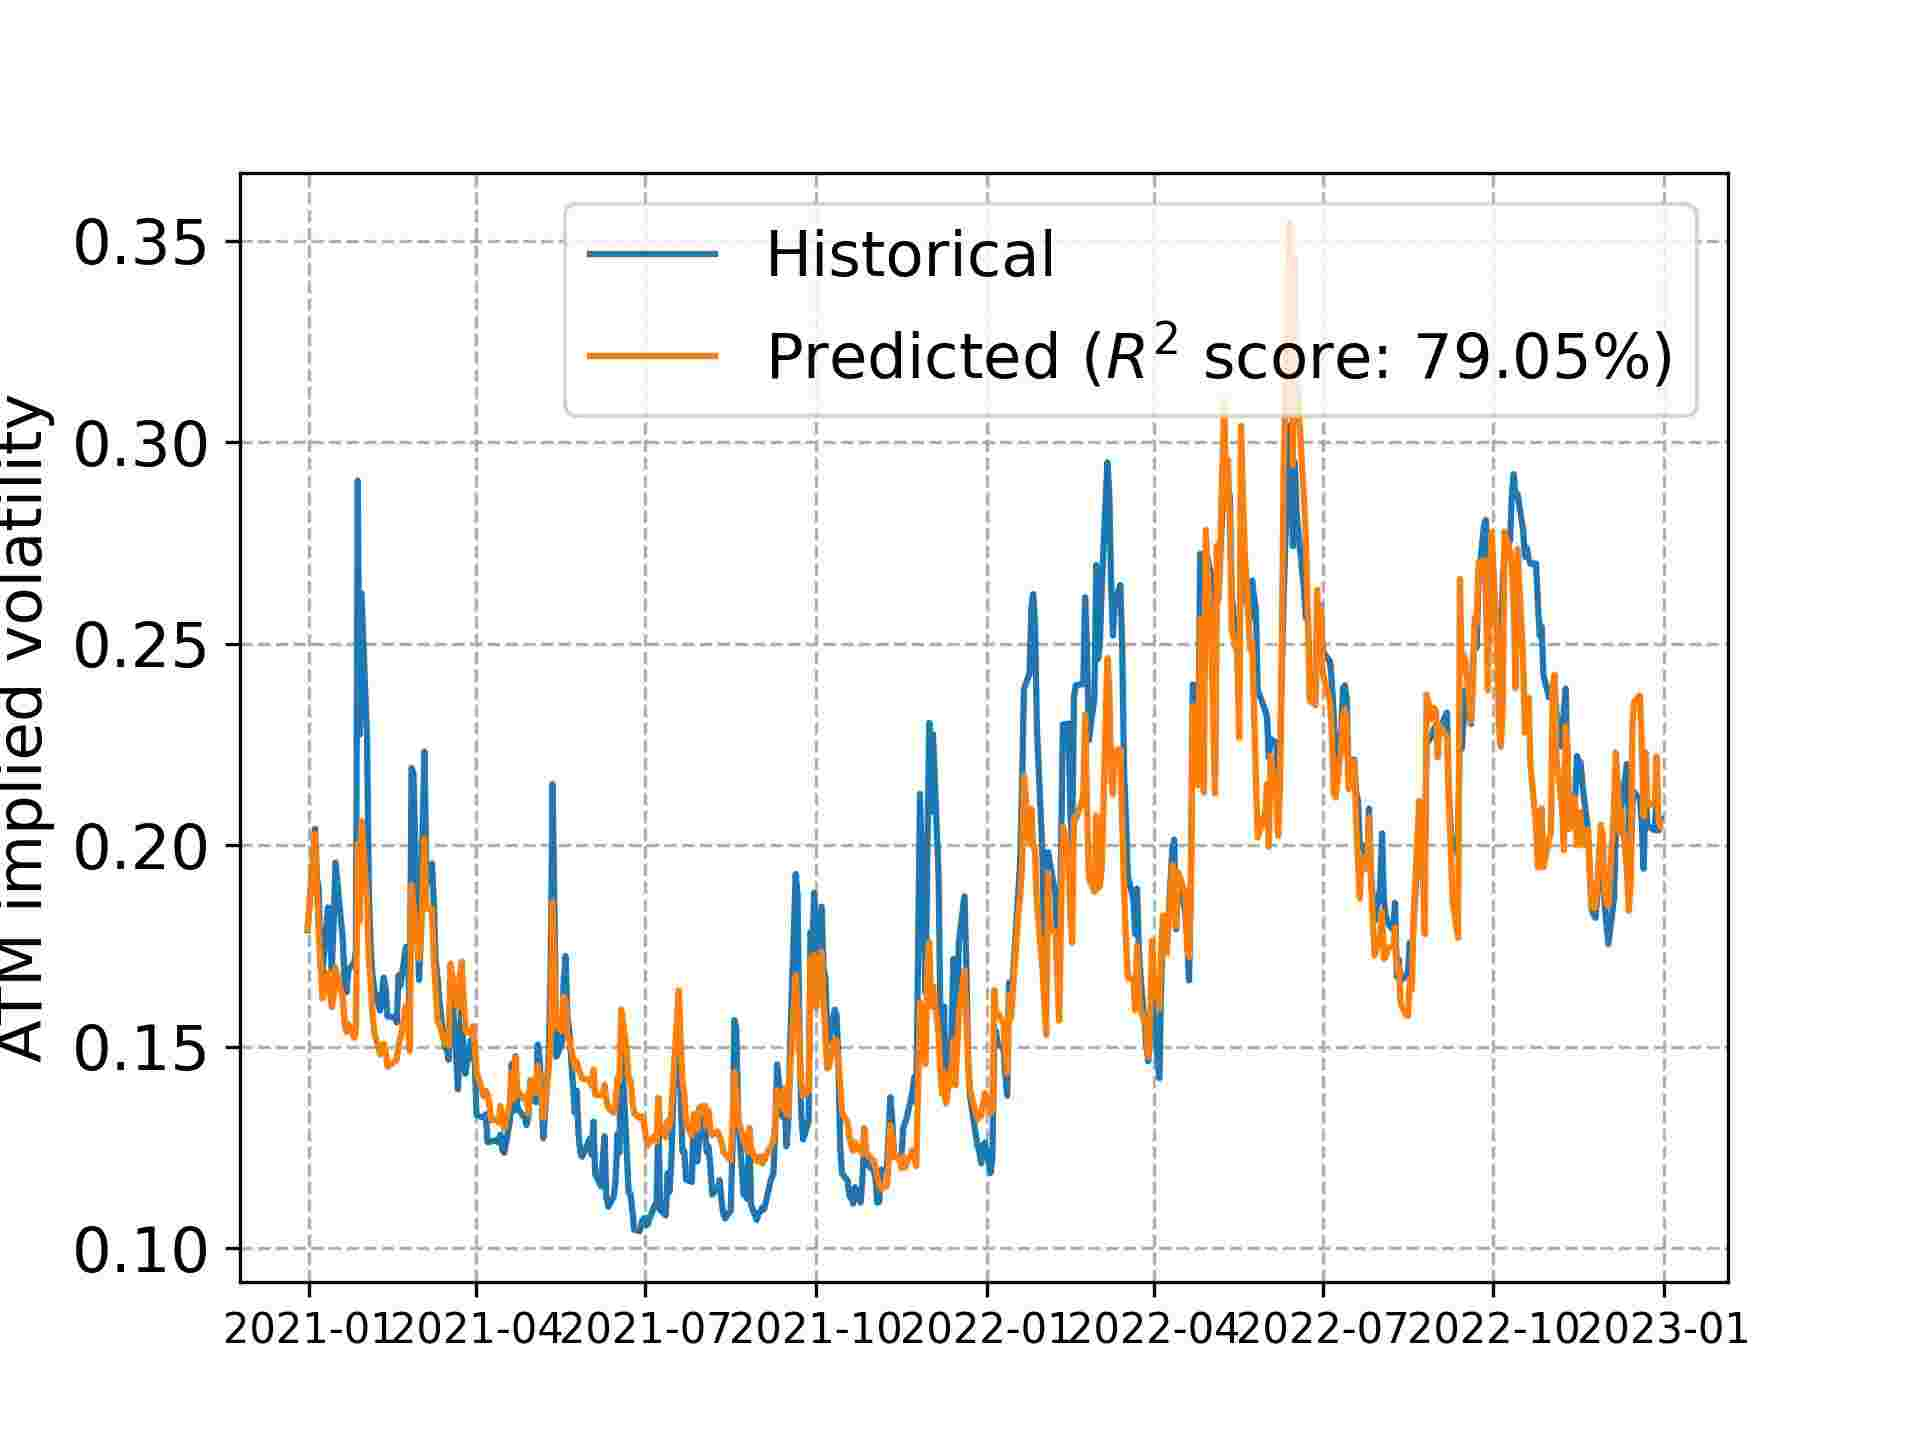
\includegraphics[width=0.3\linewidth]{SPX_ATM_IV_1M_Prediction.jpg}}
    \subfigure[12-months ATM implied volatility (S\&P 500)]{ 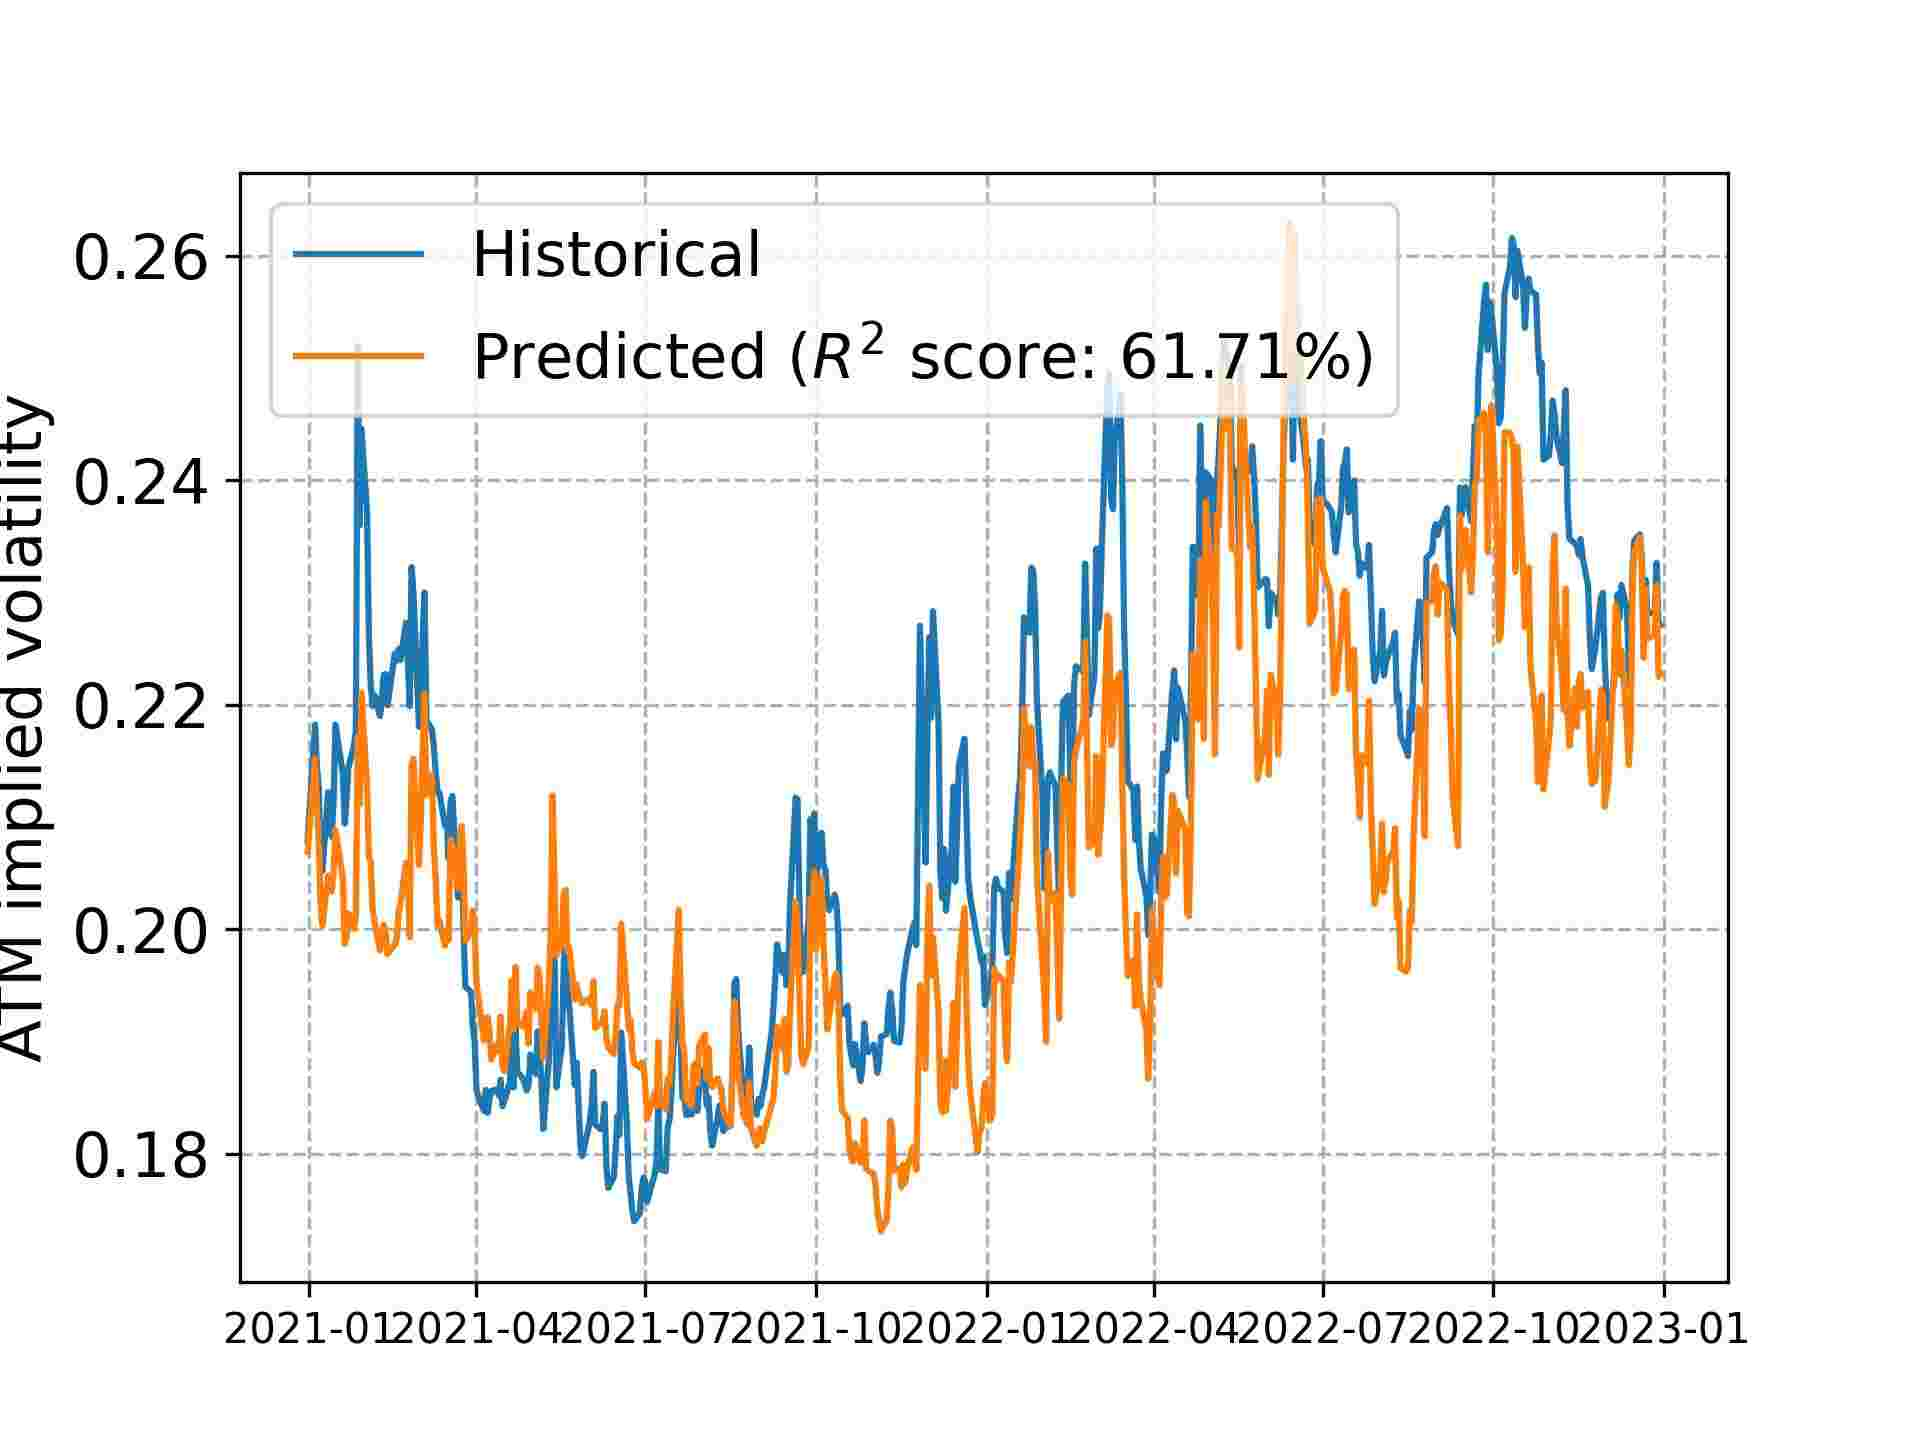
\includegraphics[width=0.3\linewidth]{SPX_ATM_IV_12M_Prediction.jpg}}
    \subfigure[24-months ATM implied volatility (S\&P 500)]{ 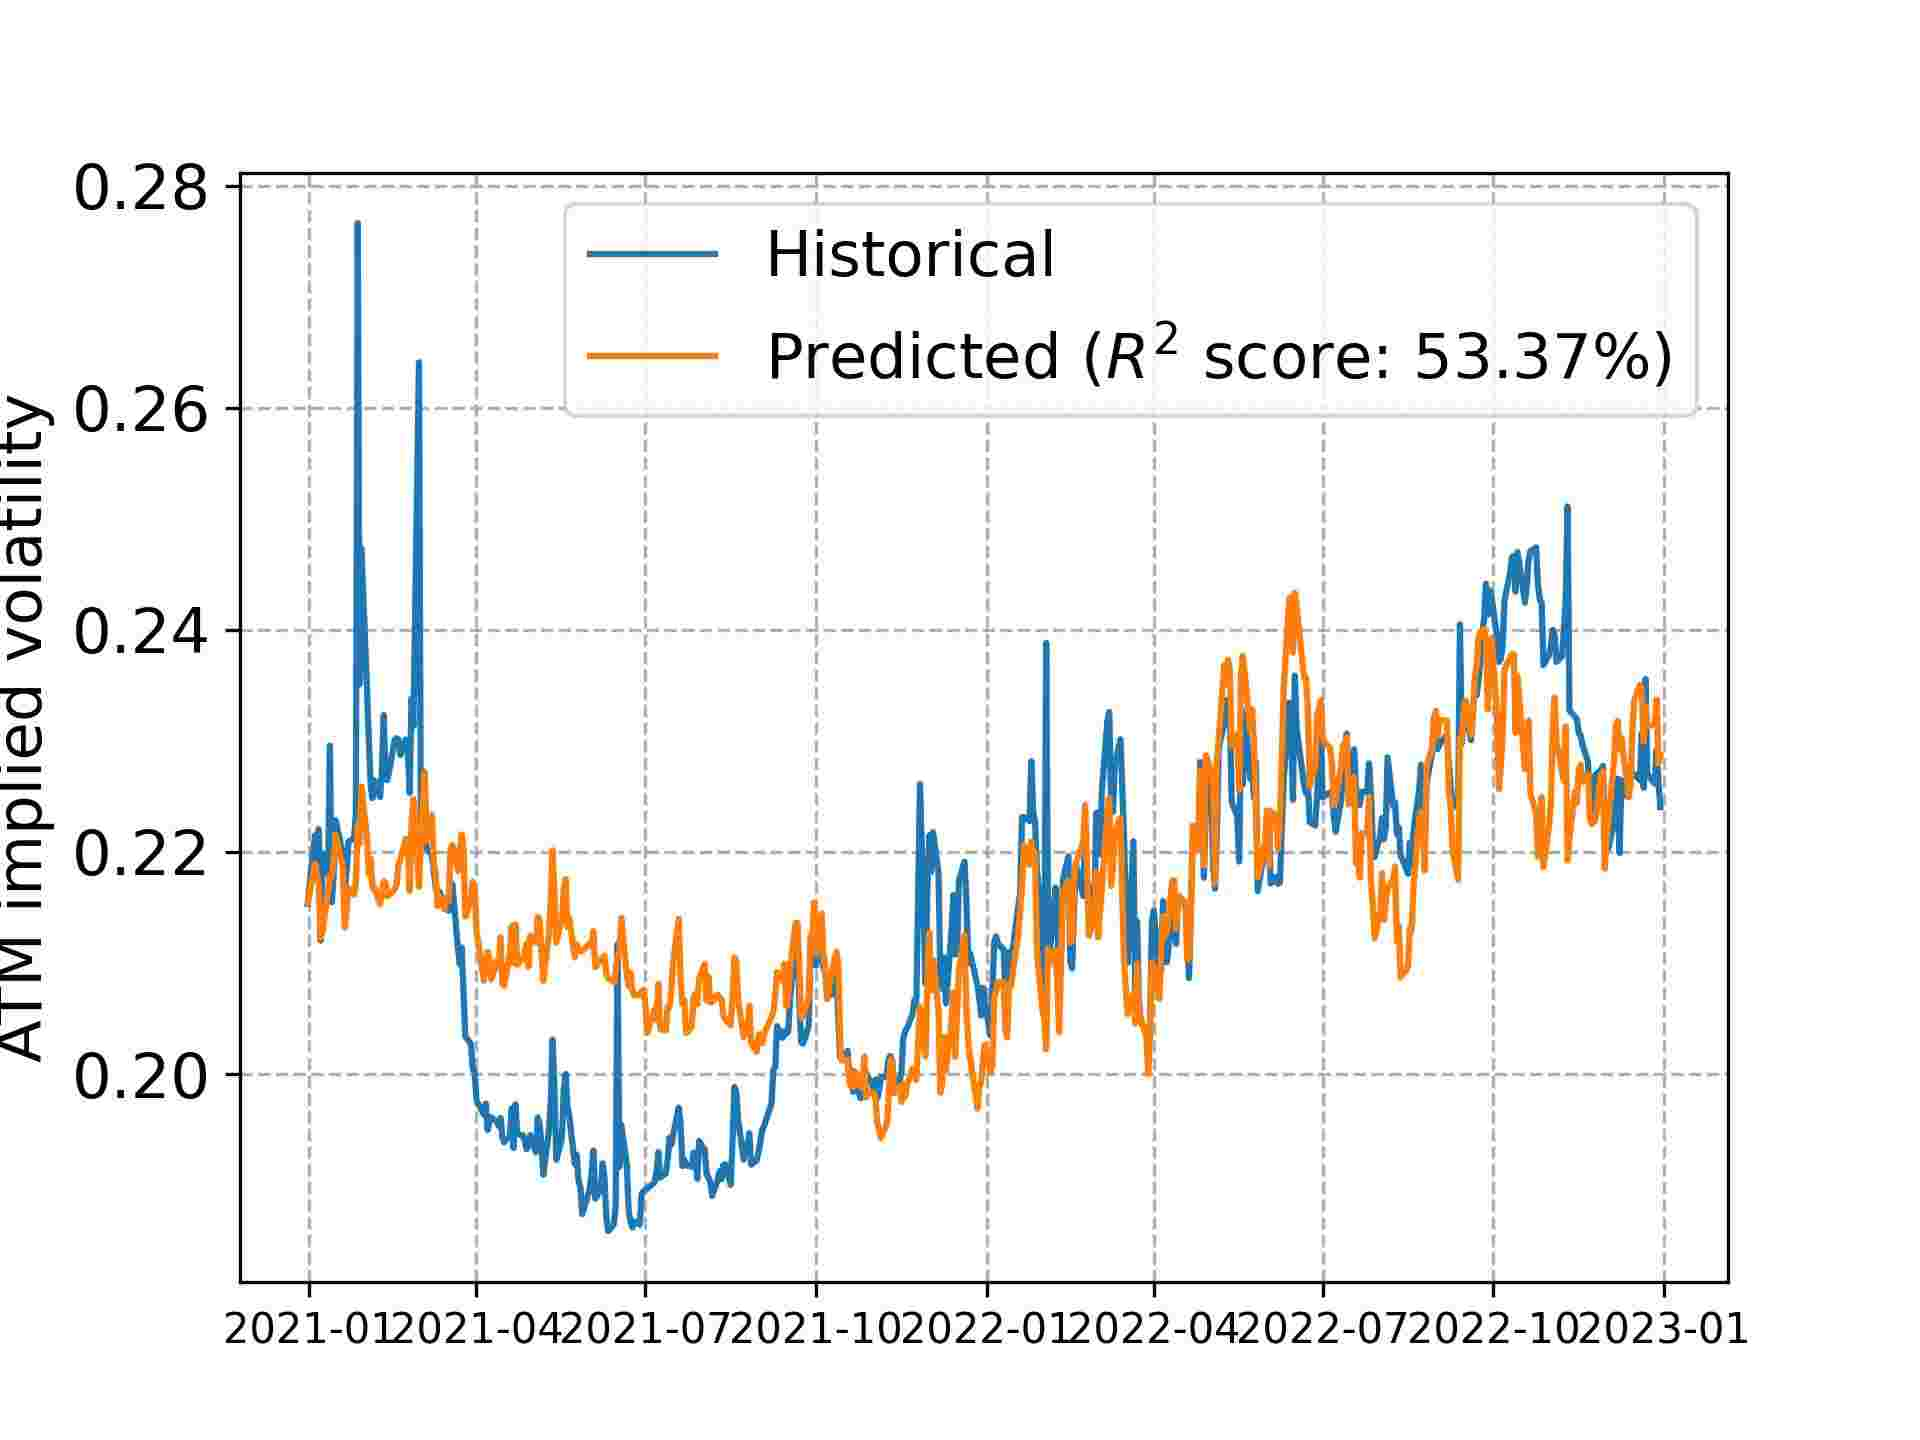
\includegraphics[width=0.3\linewidth]{SPX_ATM_IV_24M_Prediction.jpg}}
    \subfigure[1-month ATM implied volatility (Euro Stoxx 50)]{ 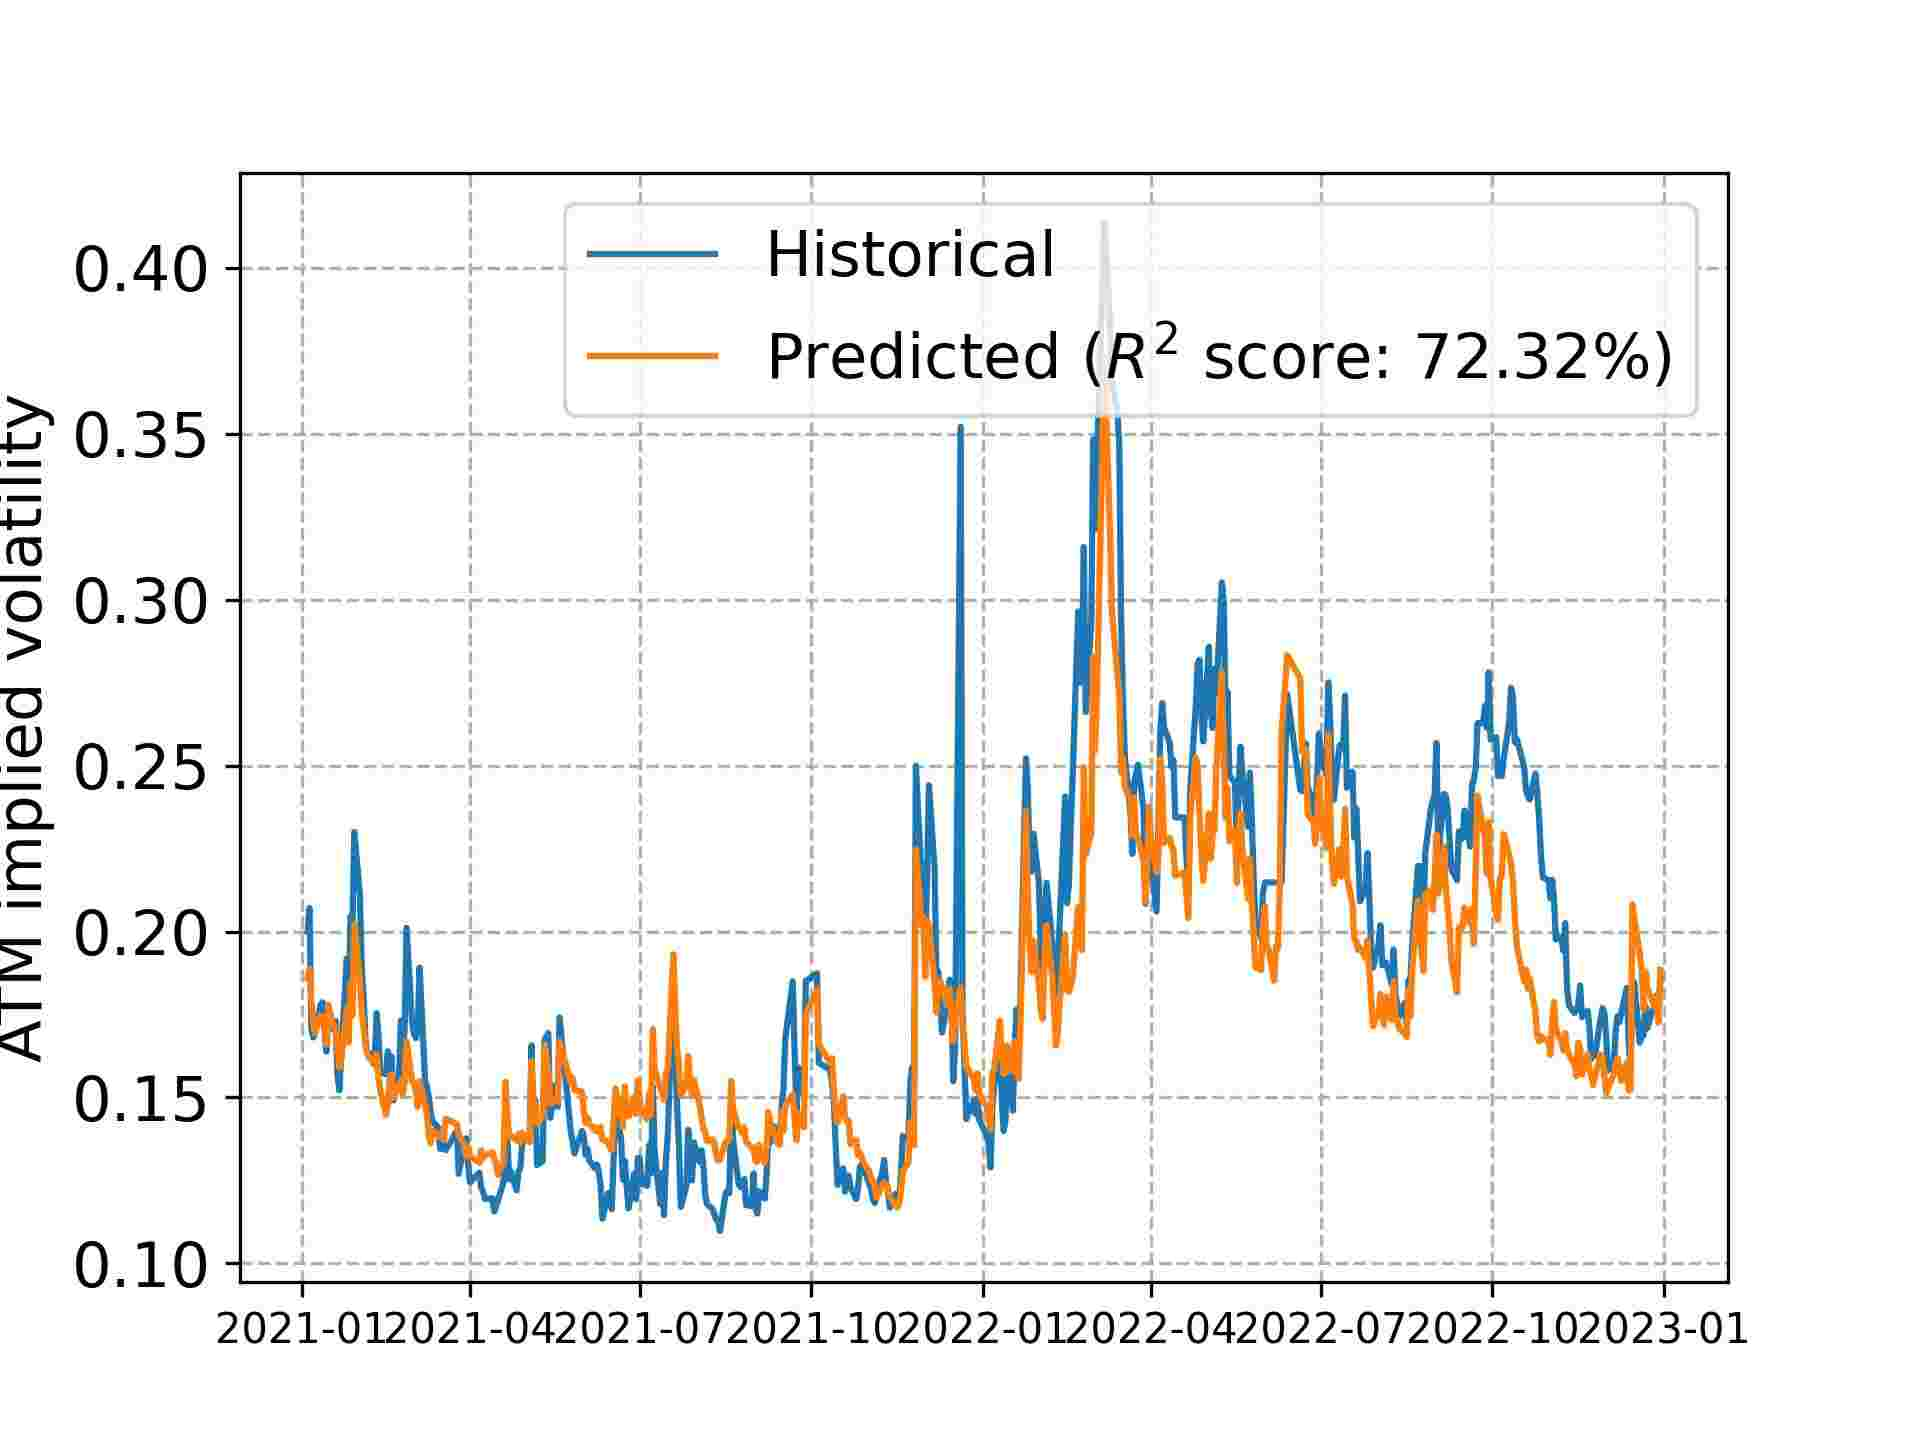
\includegraphics[width=0.3\linewidth]{STXE_ATM_IV_1M_Prediction.jpg}}
    \subfigure[12-months ATM implied volatility (Euro Stoxx 50)]{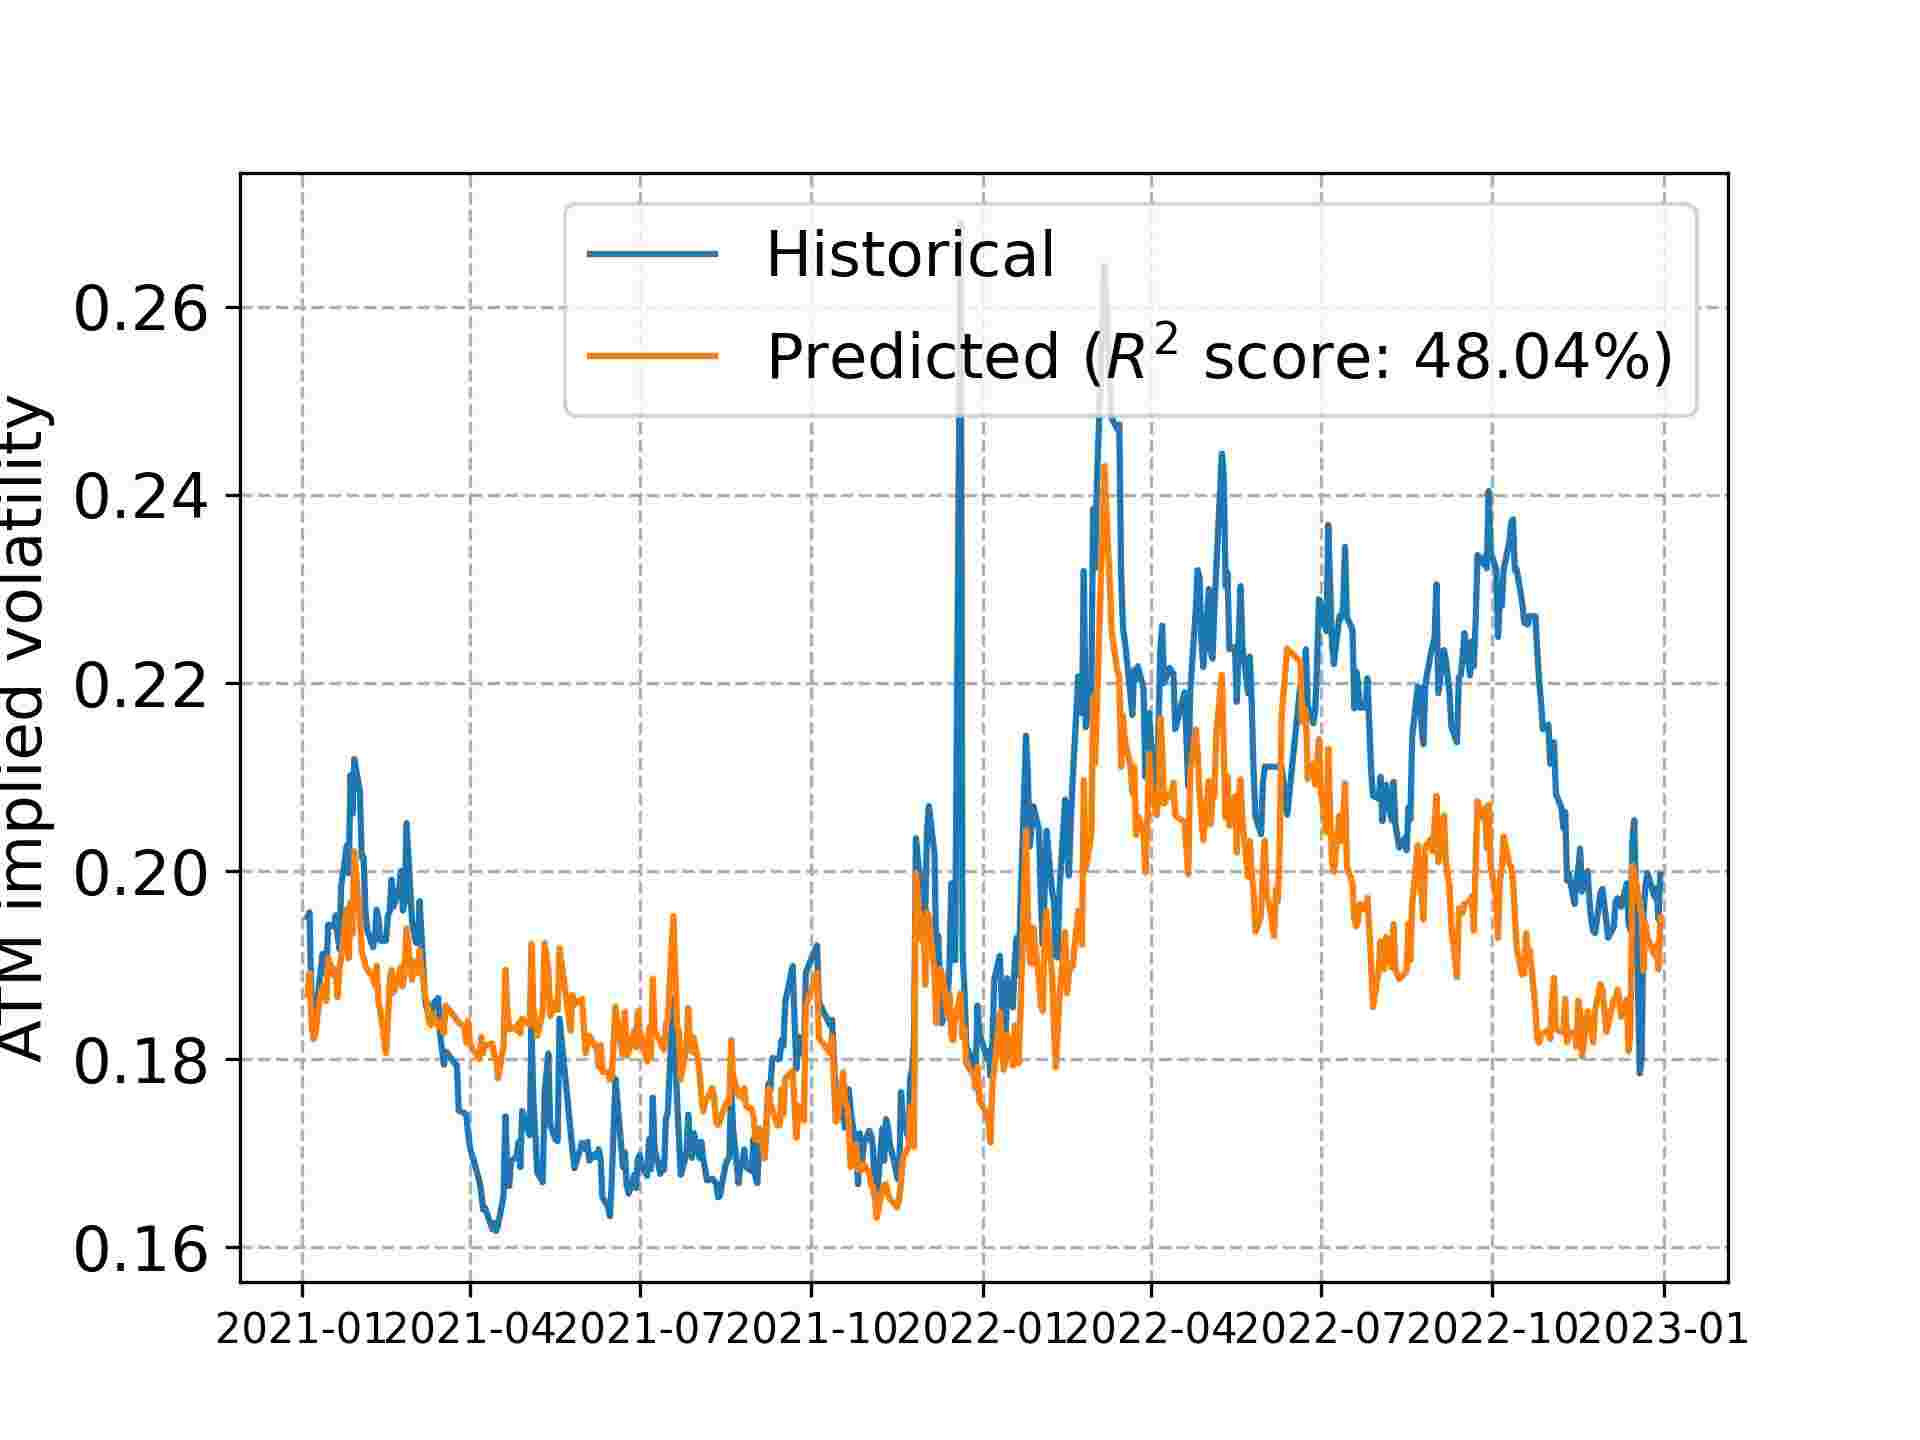
\includegraphics[width=0.3\linewidth]{STXE_ATM_IV_12M_Prediction.jpg}}
    \subfigure[24-months ATM implied volatility (Euro Stoxx 50)]{ 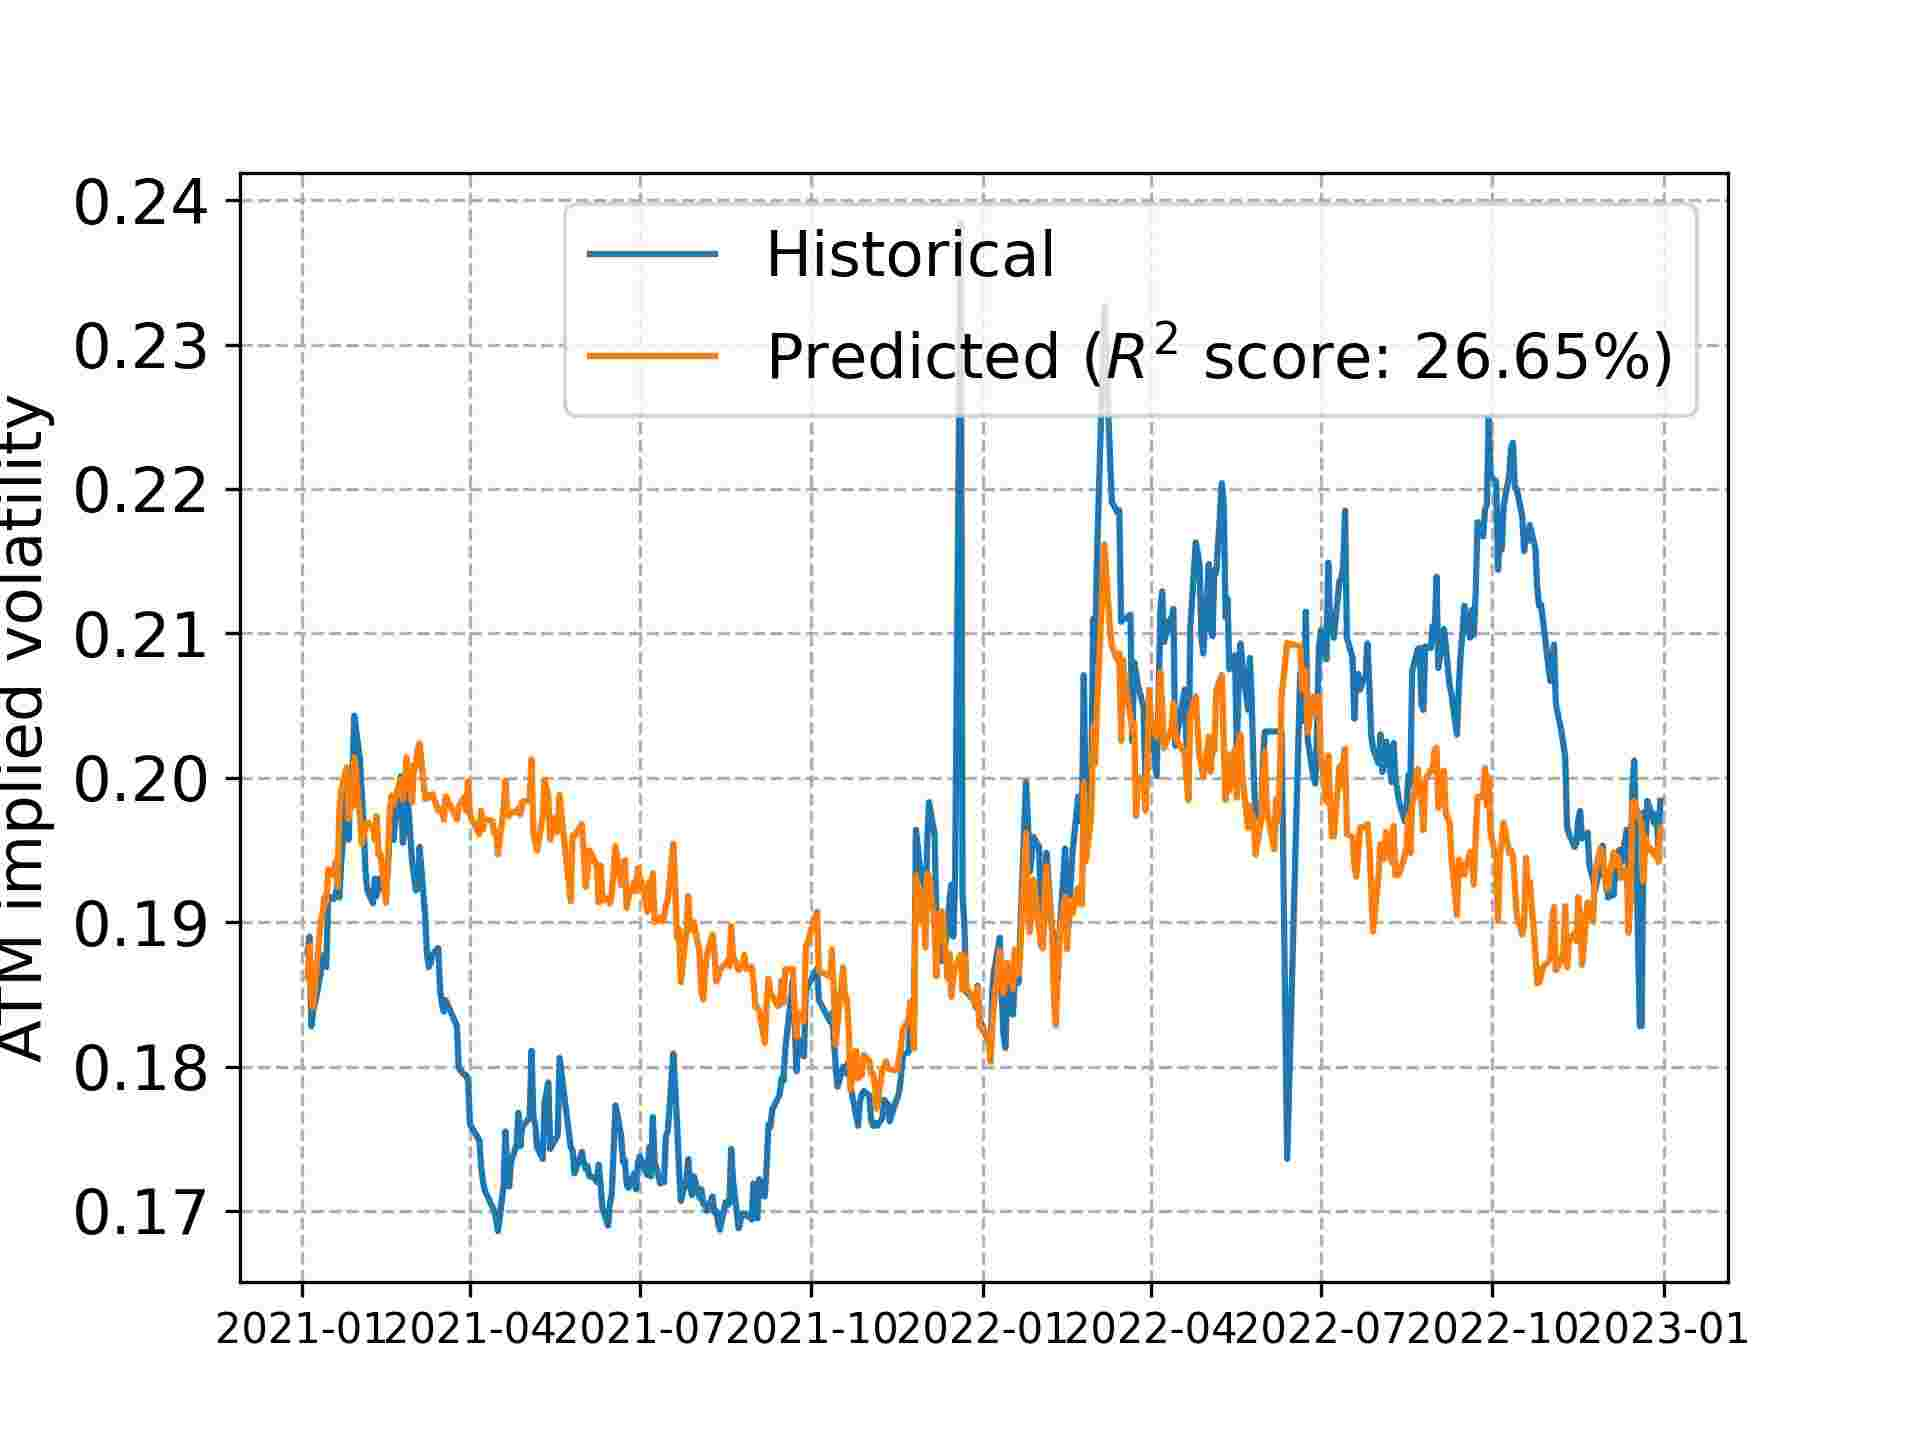
\includegraphics[width=0.3\linewidth]{STXE_ATM_IV_24M_Prediction.jpg}}
    \caption{Out-of-sample prediction of the ATM implied volatility for several time-to-maturities. The predicted ATM implied volatility is obtained by averaging the 1000 paths.}
\label{fig:iv_prediction}
\end{figure}



\subsubsection{Simulation of both the asset price and the implied volatility surface}

We now simulate the complete path-dependent SSVI model, i.e. the underlying asset price is also simulated according to Equations (\ref{eq:underlying_dynamics}). We start by performing simulations initialized using the evolution of the underlying asset price prior to the first date of the train set, namely March 8, 2012, to perform an in-sample comparison of the simulated implied volatilities with the historical ones. More precisely, we simulate 1000 paths of the asset price and the IVS over 2185 days which corresponds to the length over the train data sets. First, we show the evolution of the ATM term structure of two IVS sample paths in Figure \ref{fig:ivs_sample_paths}. As in the previous section, we obtain a very convincing evolution (in particular, we see spikes of the order of magnitude historically observed) which shows that the dynamics of the underlying asset price is also realistic. Then, in Figure \ref{fig:quantiles_envelopes}, we provide the quantile envelopes of the ATM implied volatility for the 1 month, 12 months and 24 months time-to-maturities and we compare them to the historical path of the ATM implied volatility on the train set. These graphs demonstrate that the range of simulated values is reasonable in view of the historical path since the latter exits the 0.5\%-99.5\% quantile envelopes with a frequency that is smaller than 1\%. Note however that the simulated values implied volatilities are in average a bit larger than the historical ones which is purely due to the simulation of the asset price in view of the results presented in Section \ref{sec:cond_simus} where the average implied volatilities are at the right level. We now move to the out-of-sample evaluation of the path-dependent SSVI model. To this end, we perform simulations starting from the evolution of the underlying asset price prior to the start date of the test set, namely January 1, 2021. We consider again 1000 sample paths but we now make the simulations over 504 days corresponding to the length of the test sets. In Figure \ref{fig:quantiles_envelopes_oos}, we provide the quantile envelopes of the ATM implied volatility for the 1 month, 12 months and 24 months time-to-maturities and we compare them to the historical path of the ATM implied volatility on the test set. In this case, the range of the simulated values is again satisfying and the average simulated value is very close the historical one. In Figure \ref{fig:average_ivs}, we compare the historical average IVS on the test set to the simulated average IVS allowing a comparison beyond the ATM implied volatilities. The overall shapes are very close and the average absolute difference between the historical average surface and the simulated one is 0.6\% for the S\&P 500 and 1\% for the Euro Stoxx 50 which shows the simulated away-from-the-money implied volatilities are also consistent with historical data. \\

\begin{figure}
    \centering
    \subfigure[Sample path of the S\&P 500 ATM term structure]{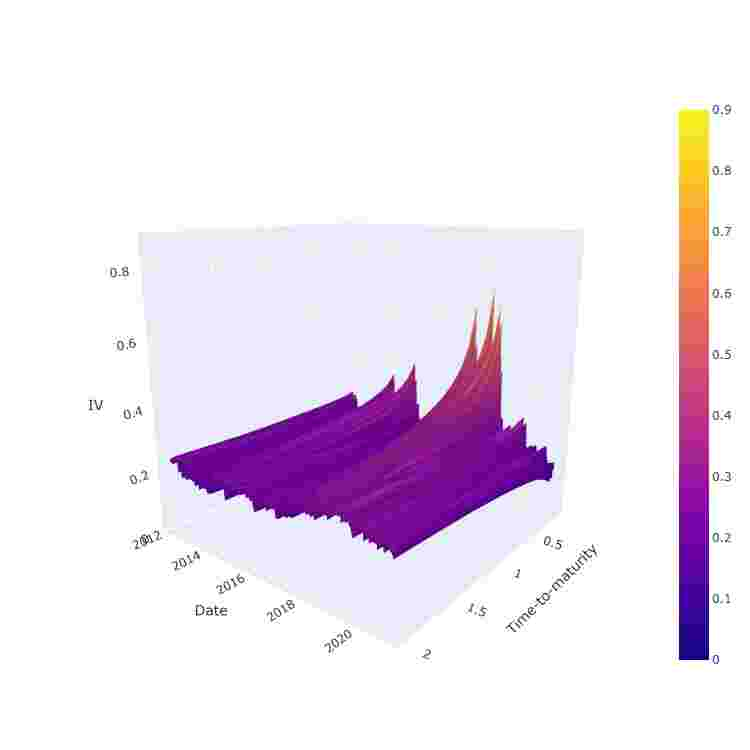
\includegraphics[width=0.45\linewidth]{SPX_ATM_Simu_IV.jpg}}
    \subfigure[Sample path of the Euro Stoxx 50 ATM term structure]{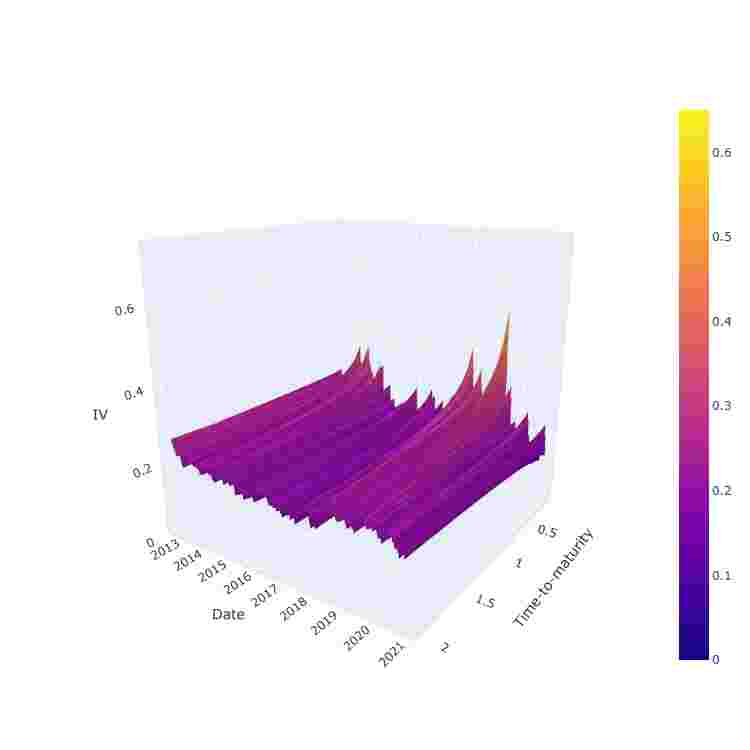
\includegraphics[width=0.45\linewidth]{SX5E_ATM_Simu_IV.jpg}}
    \caption{ATM term structure for two IVS sample paths in the complete path-dependent SSVI model.}
\label{fig:ivs_sample_paths}
\end{figure}



\begin{figure}
    \centering
    \subfigure[1-month ATM implied volatility (S\&P 500)]{ 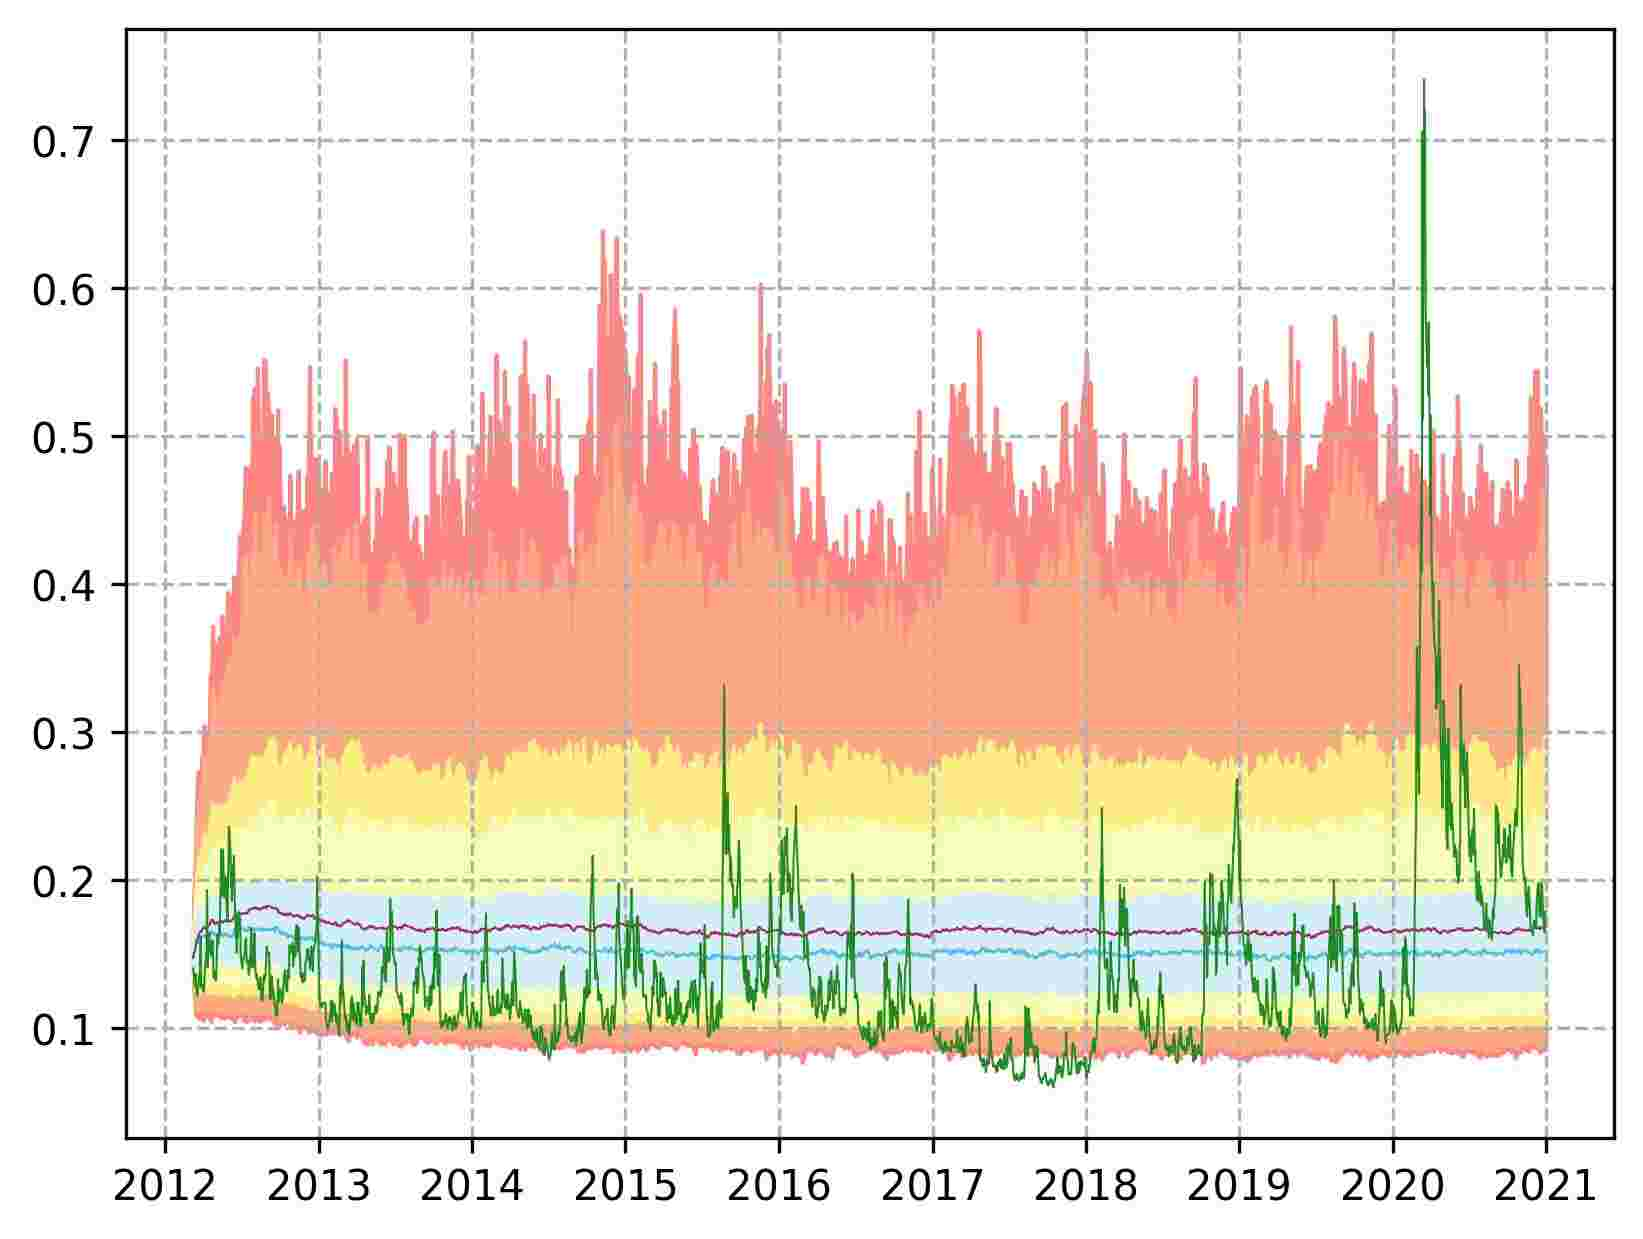
\includegraphics[width=0.25\linewidth]{SPX_ATM_1M_In_Sample.jpg}}
    \subfigure[12-months ATM implied volatility (S\&P 500)]{ 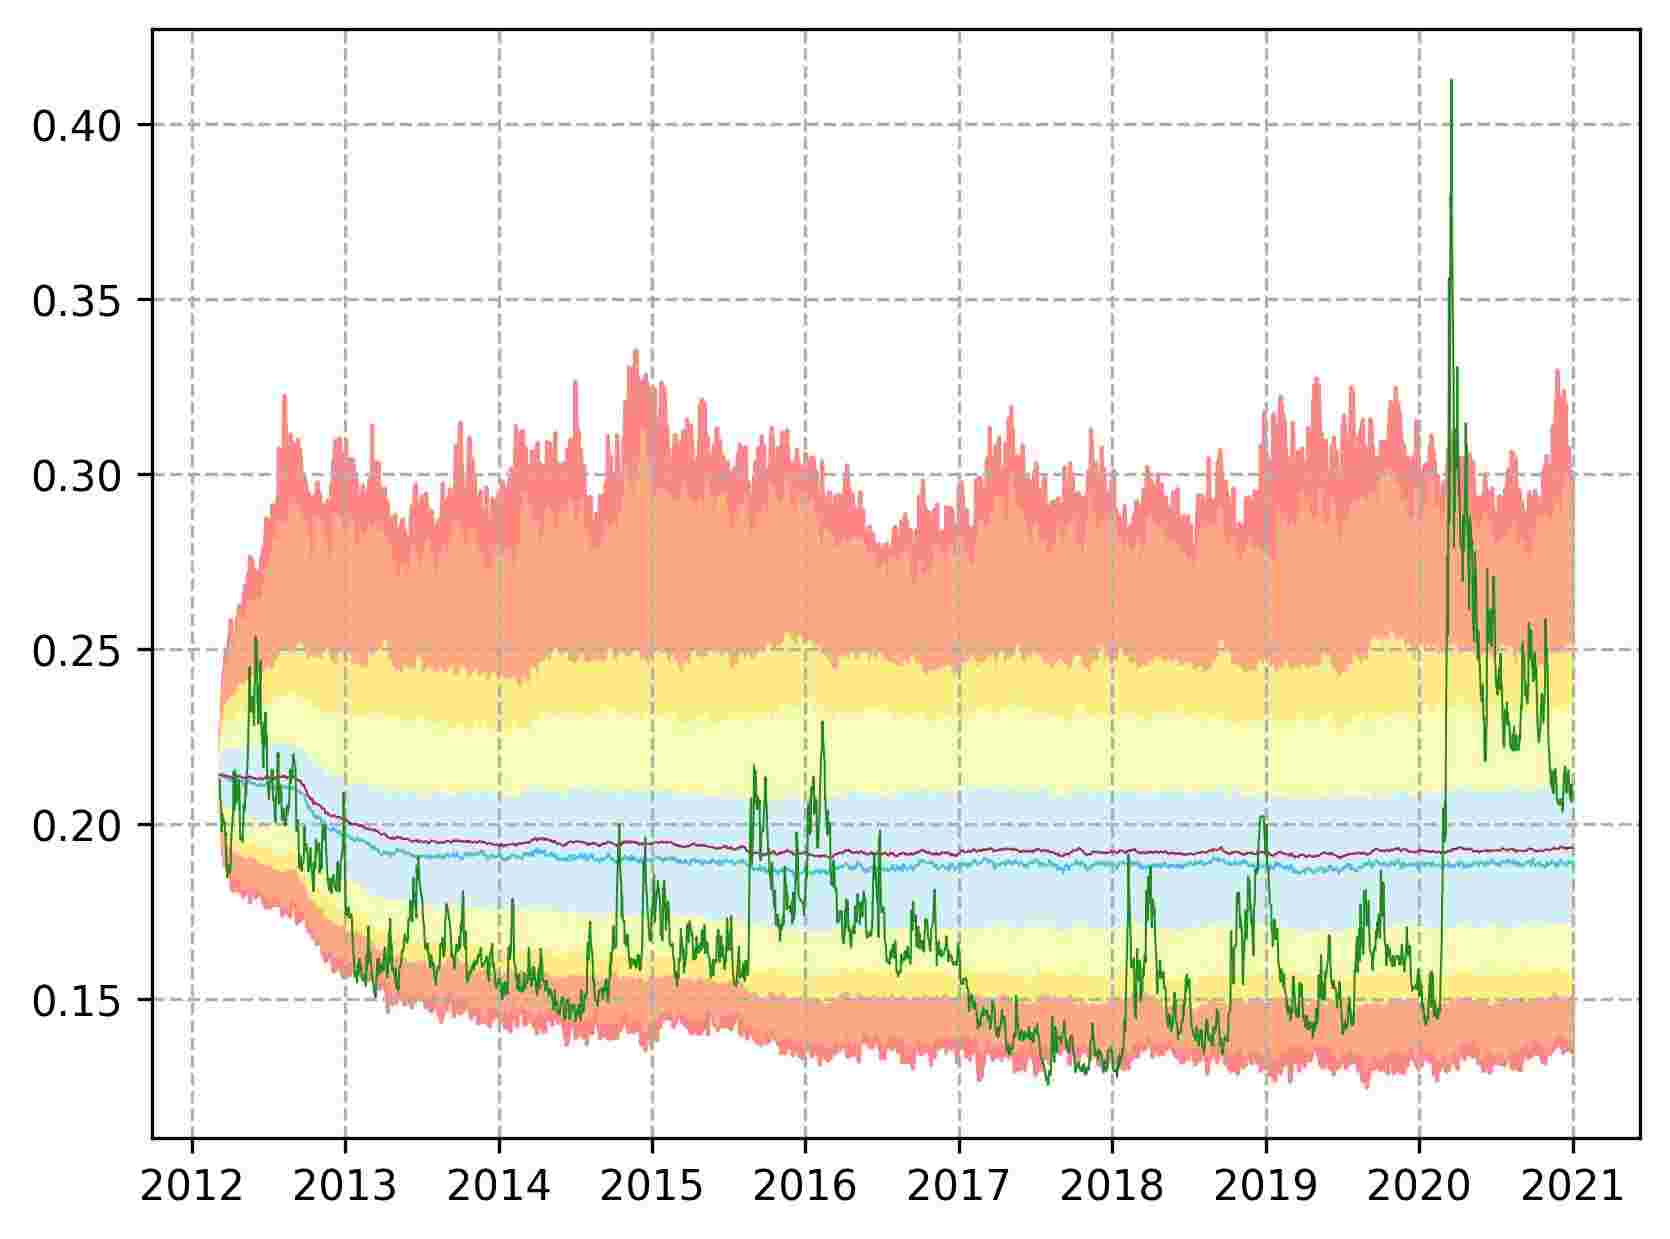
\includegraphics[width=0.25\linewidth]{SPX_ATM_12M_In_Sample.jpg}}
    \subfigure[24-months ATM implied volatility (S\&P 500)]{ 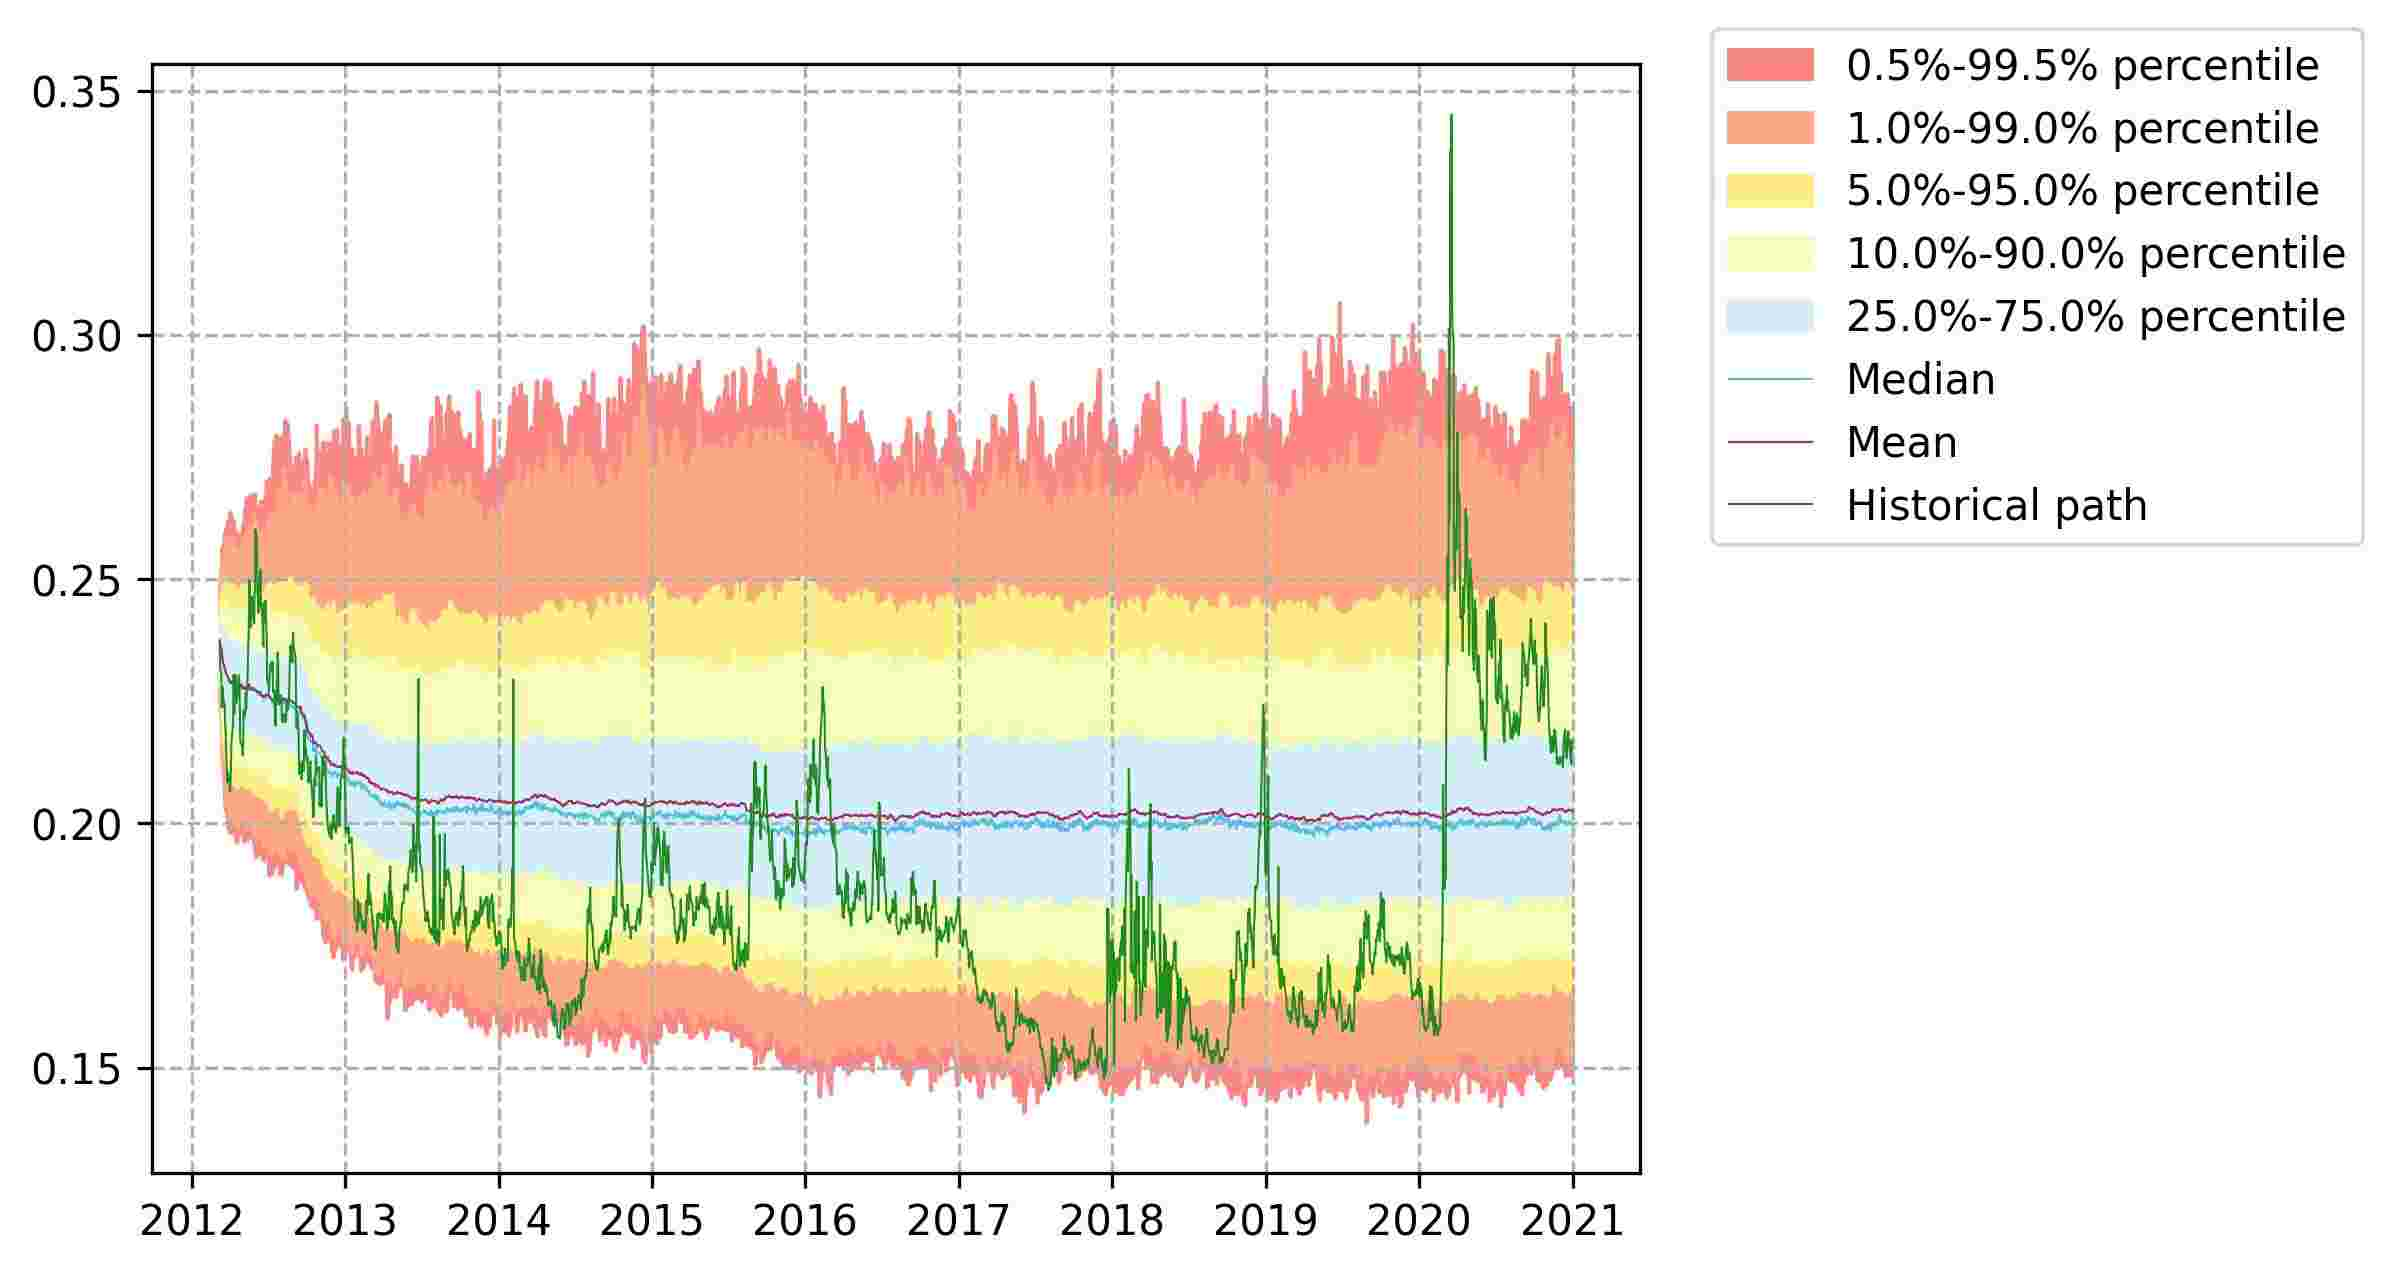
\includegraphics[width=0.36\linewidth]{SPX_ATM_24M_In_Sample.jpg}}
    \subfigure[1-month ATM implied volatility (Euro Stoxx 50)]{ 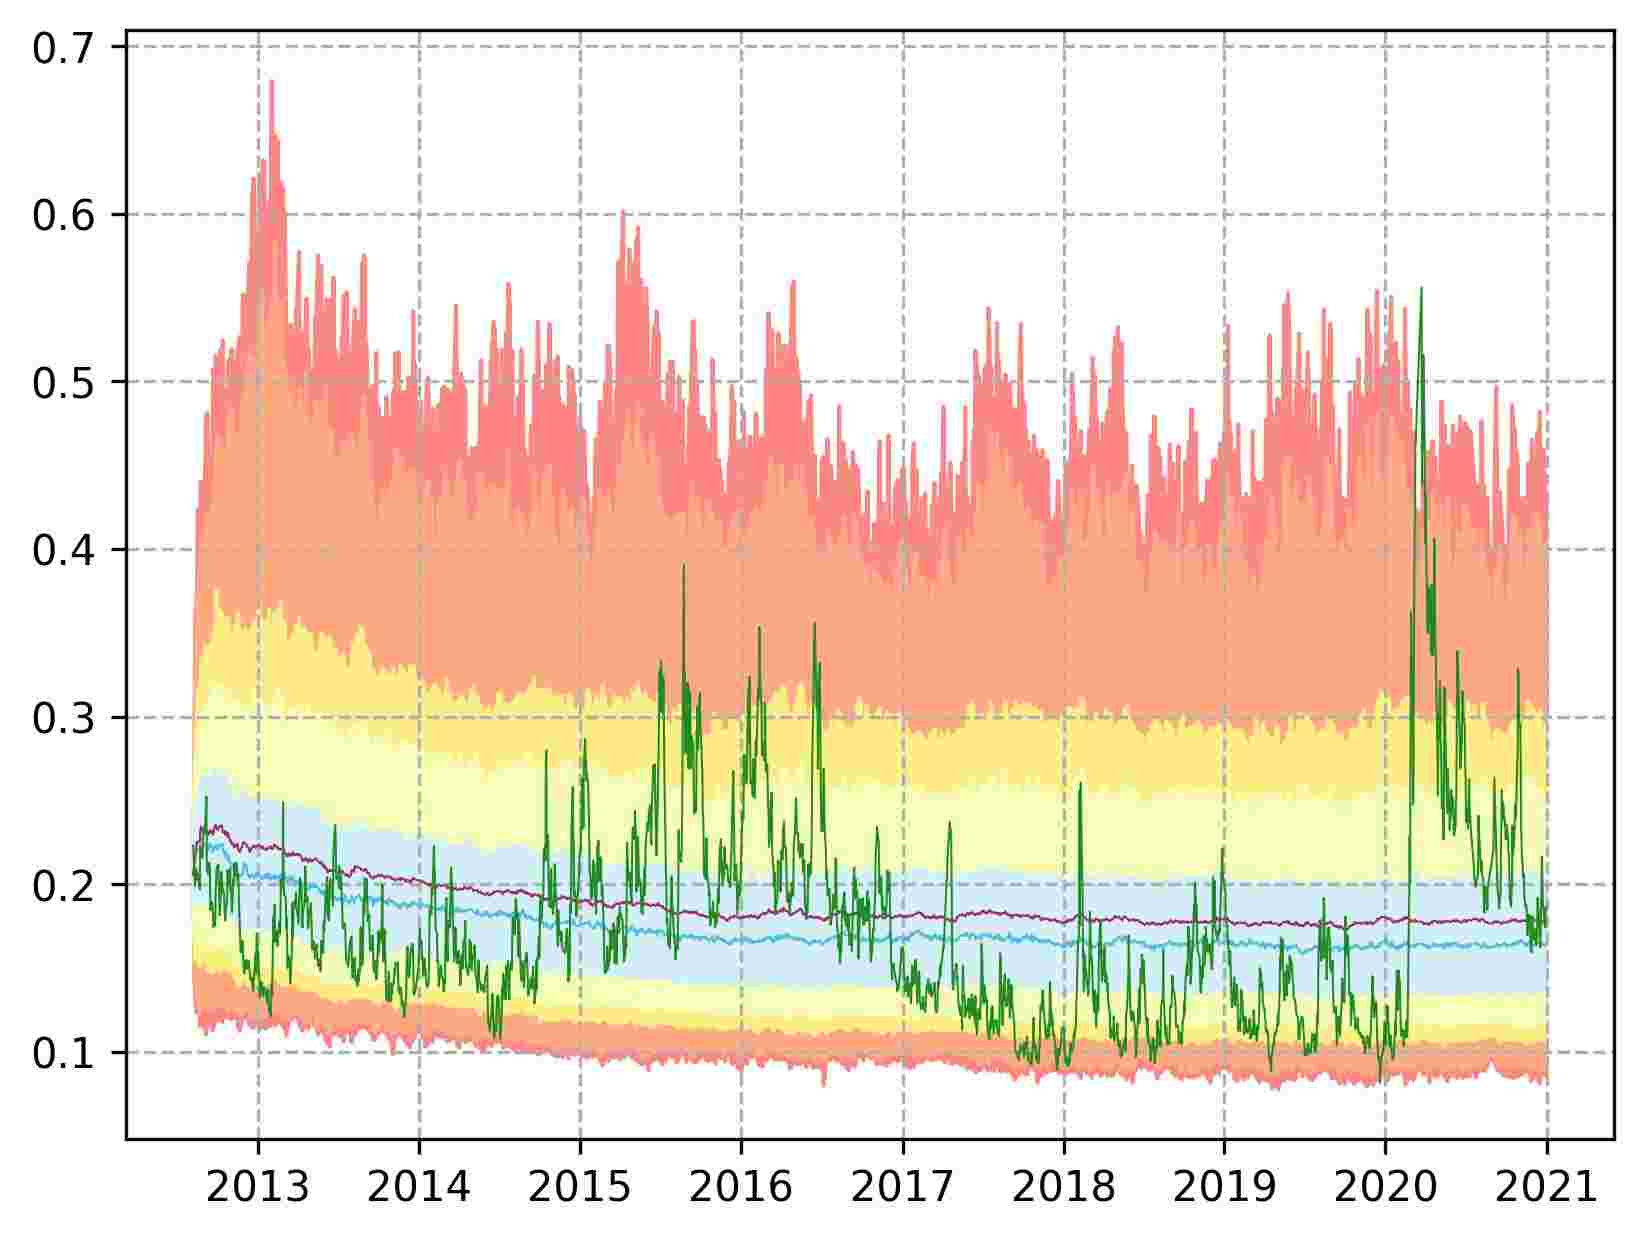
\includegraphics[width=0.25\linewidth]{STXE_ATM_1M_In_Sample.jpg}}
    \subfigure[12-months ATM implied volatility (Euro Stoxx 50)]{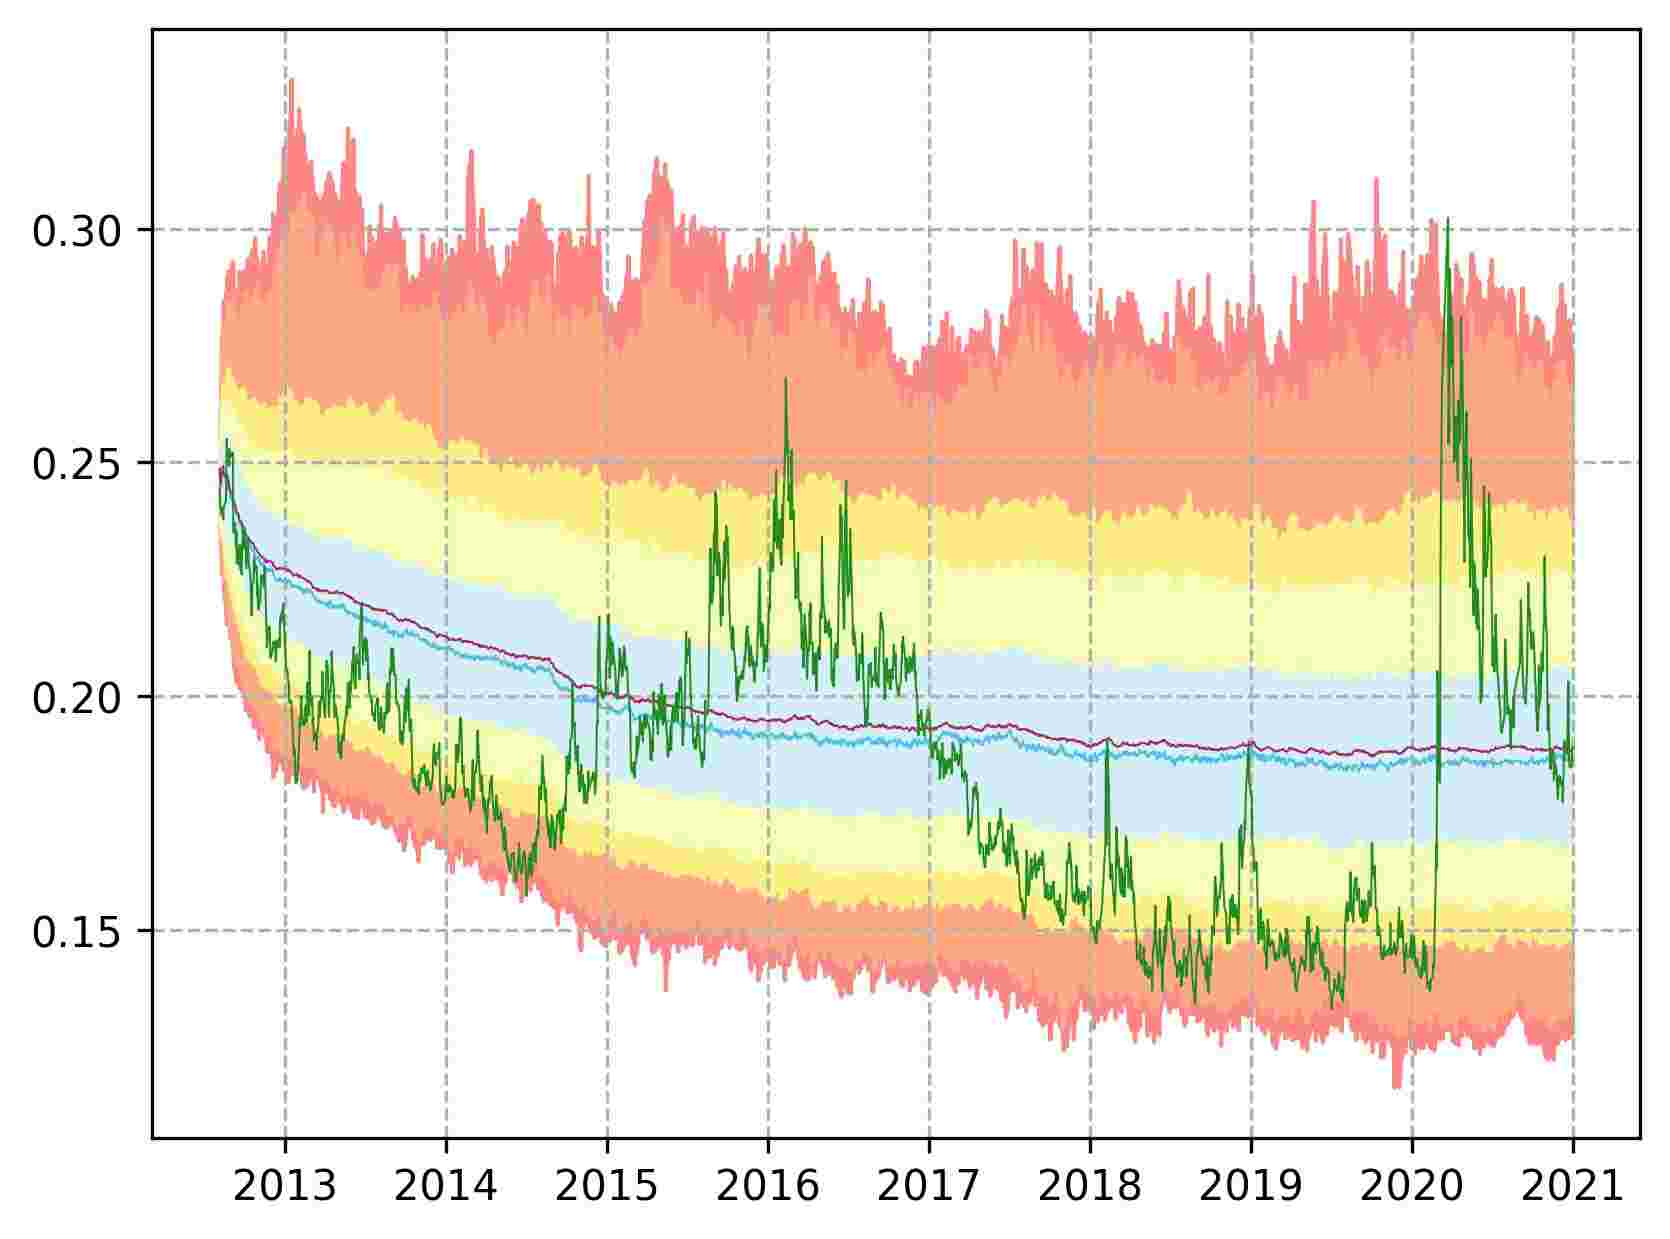
\includegraphics[width=0.25\linewidth]{STXE_ATM_12M_In_Sample.jpg}}
    \subfigure[24-months ATM implied volatility (Euro Stoxx 50)]{ 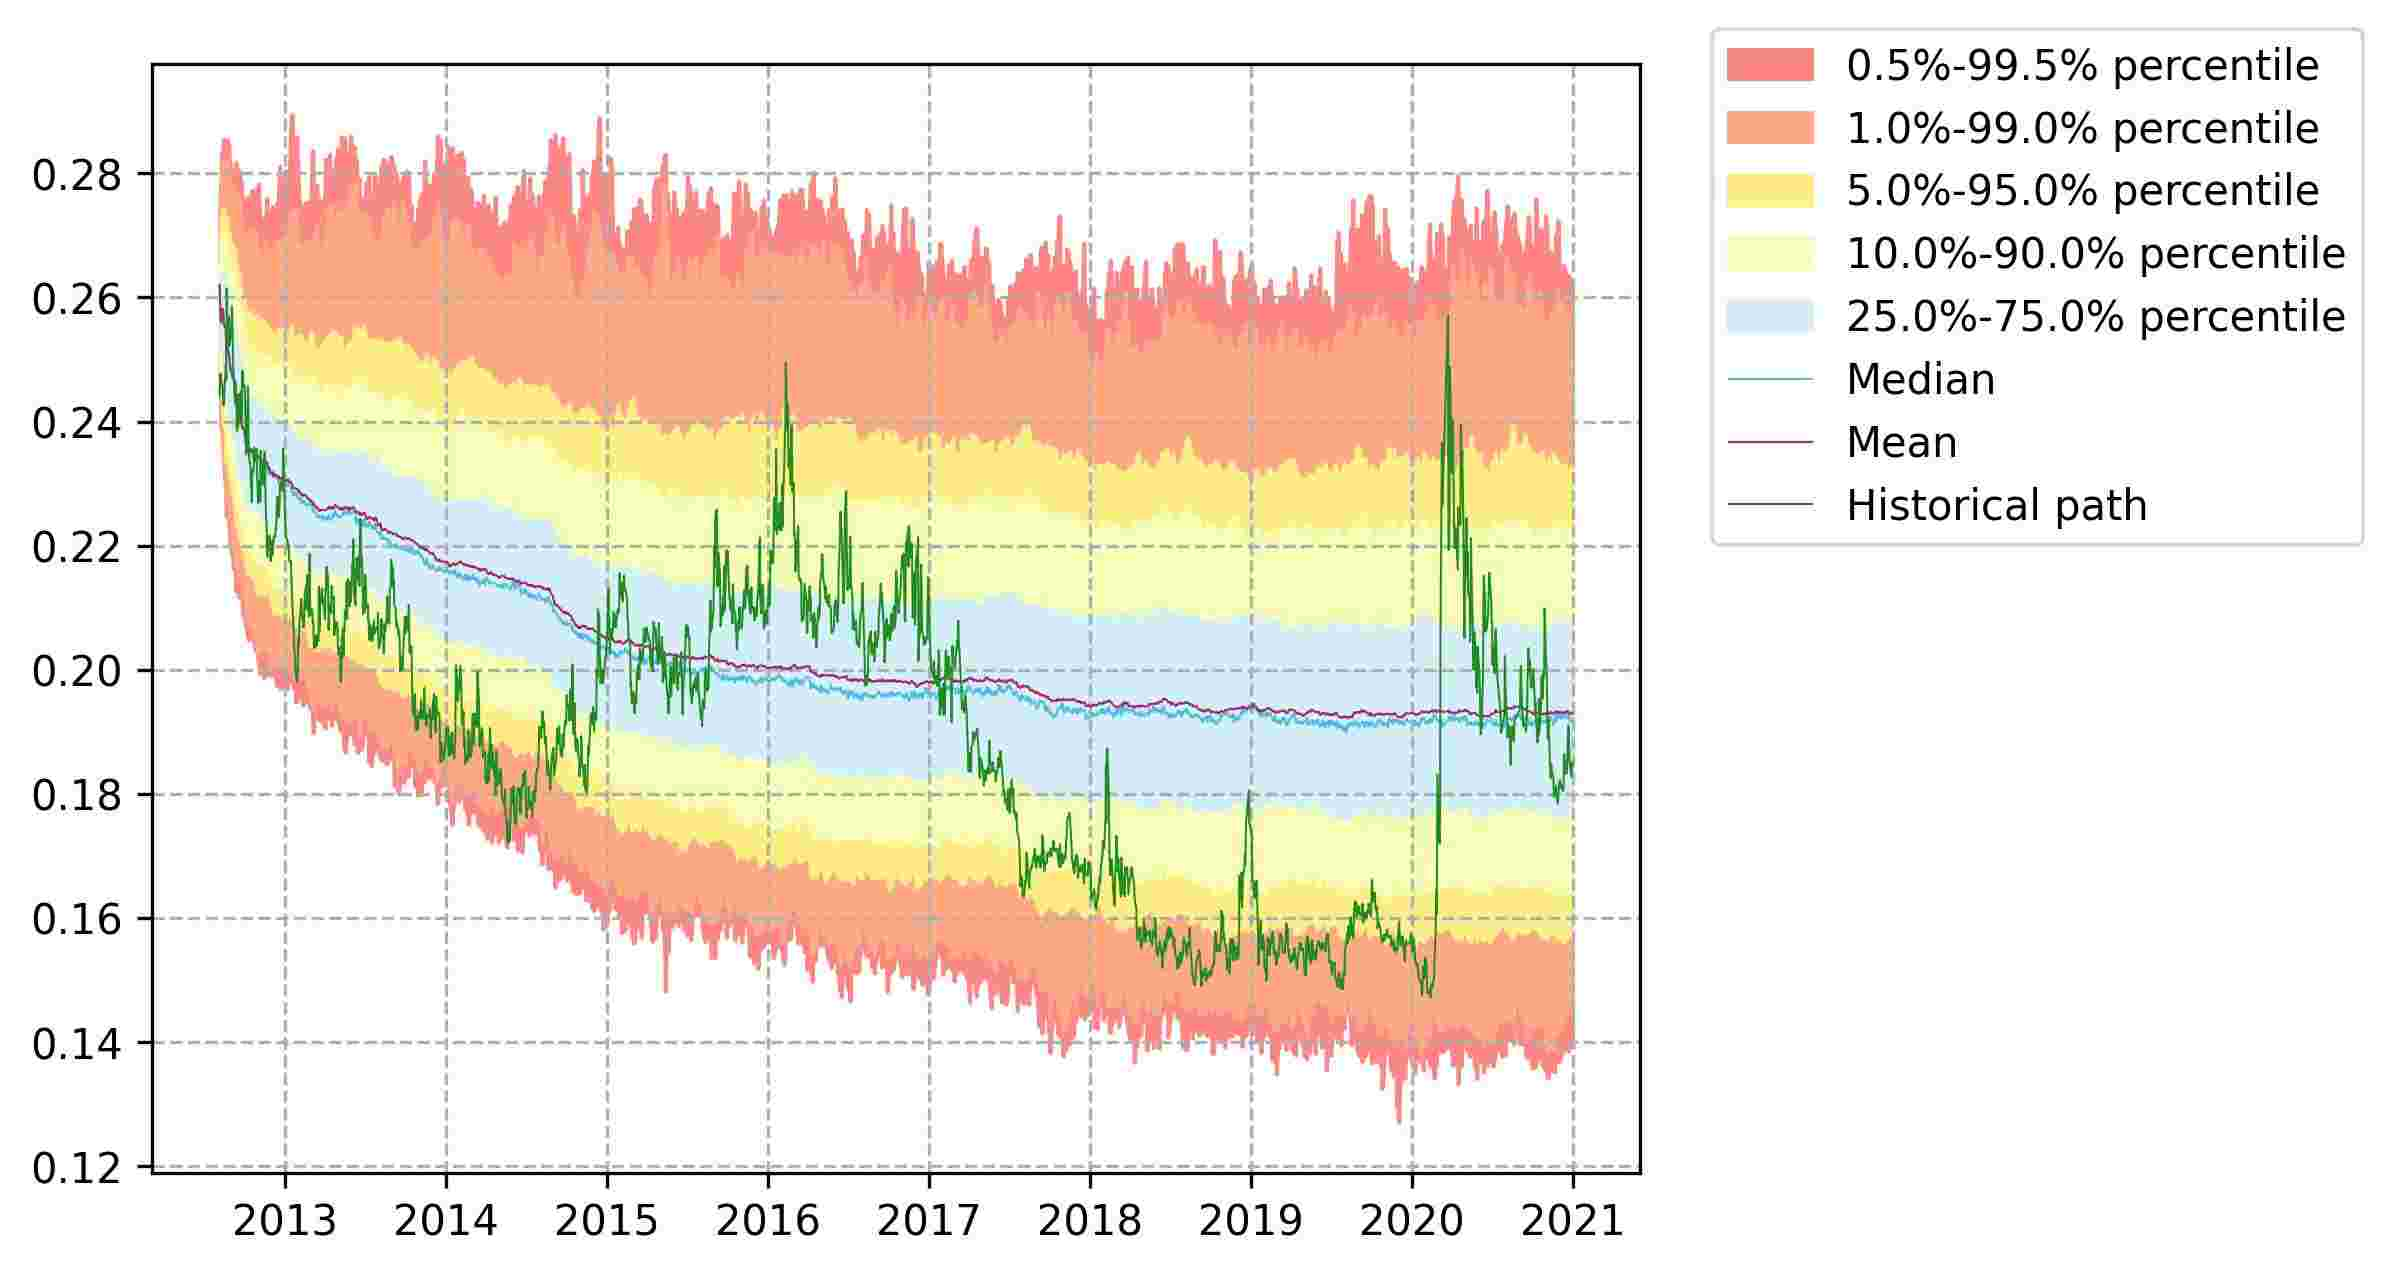
\includegraphics[width=0.36\linewidth]{STXE_ATM_24M_In_Sample.jpg}}
    \caption{In-sample quantiles envelopes of the ATM implied volatility for several time-to-maturities. }
\label{fig:quantiles_envelopes}
\end{figure}

\begin{figure}
    \centering
    \subfigure[1-month ATM implied volatility (S\&P 500)]{ 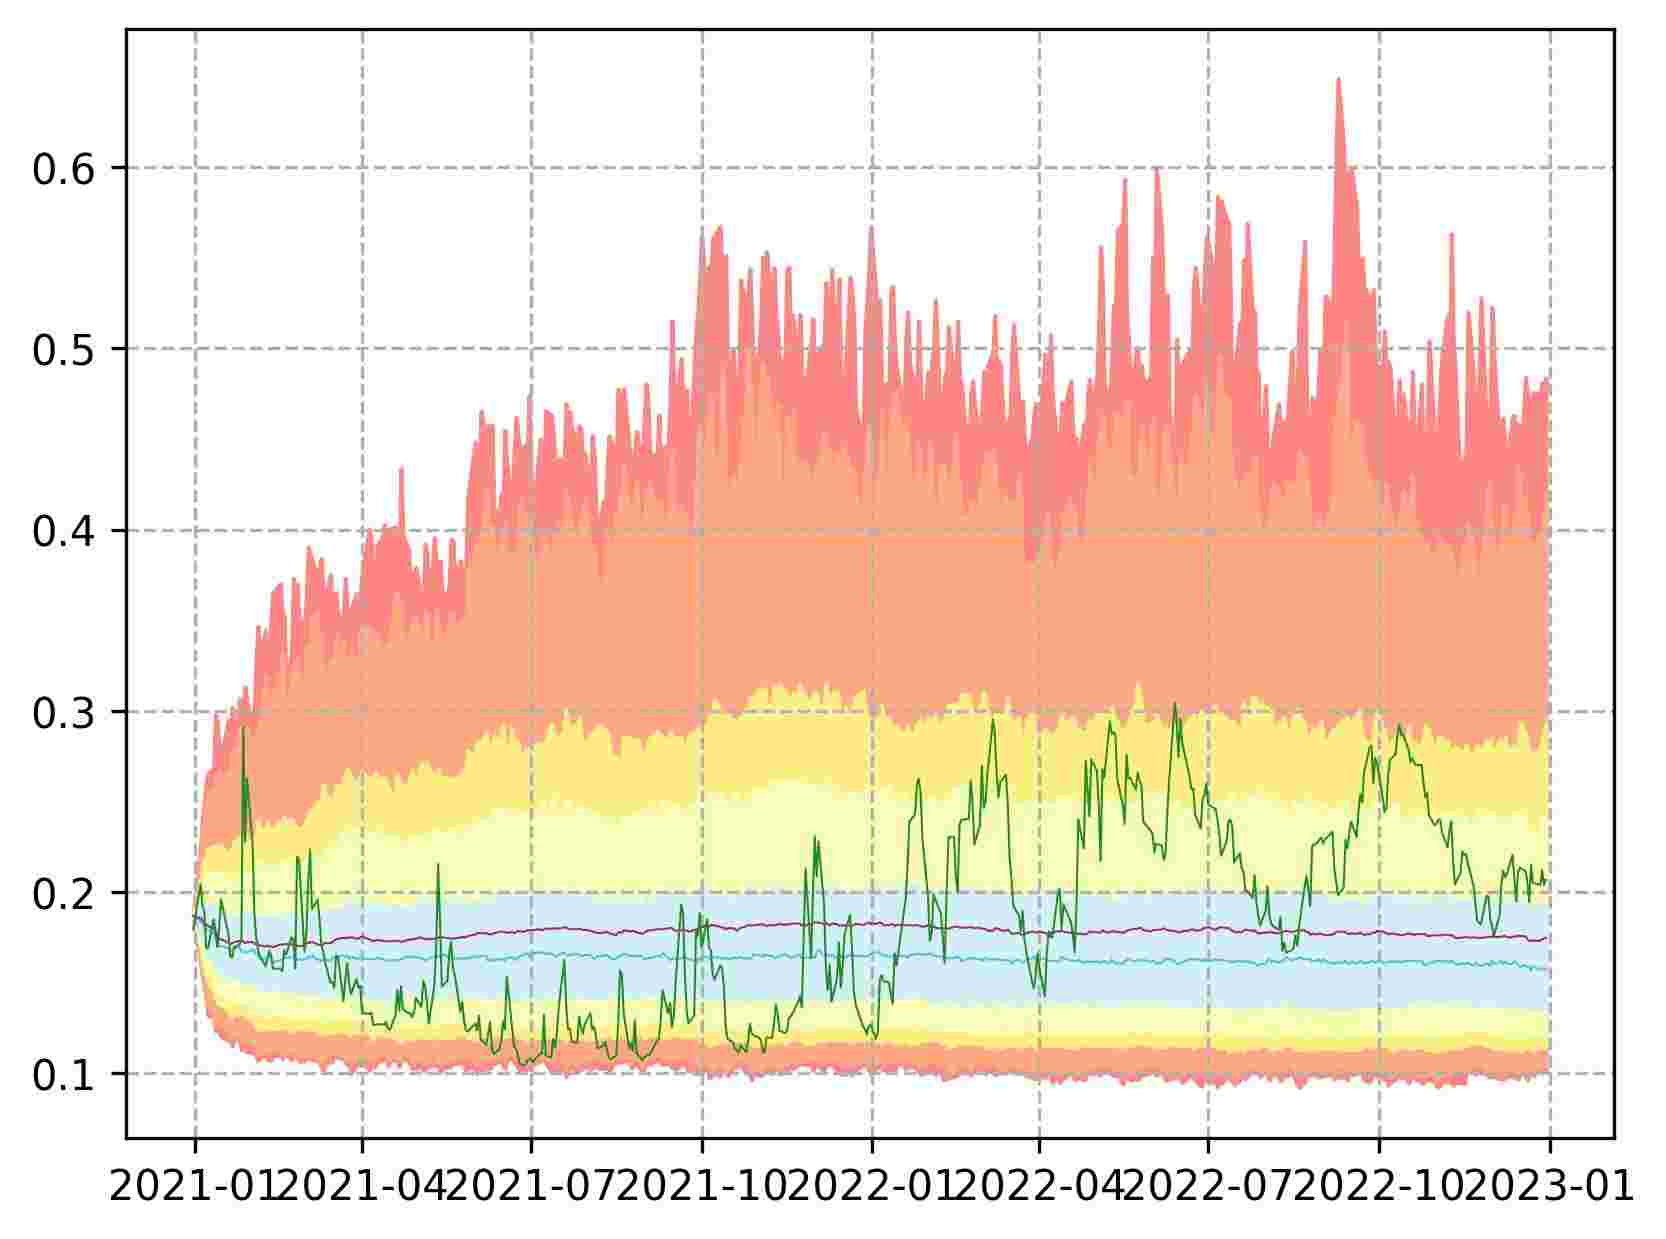
\includegraphics[width=0.25\linewidth]{SPX_ATM_1M_Out_Sample.jpg}}
    \subfigure[12-months ATM implied volatility (S\&P 500)]{ 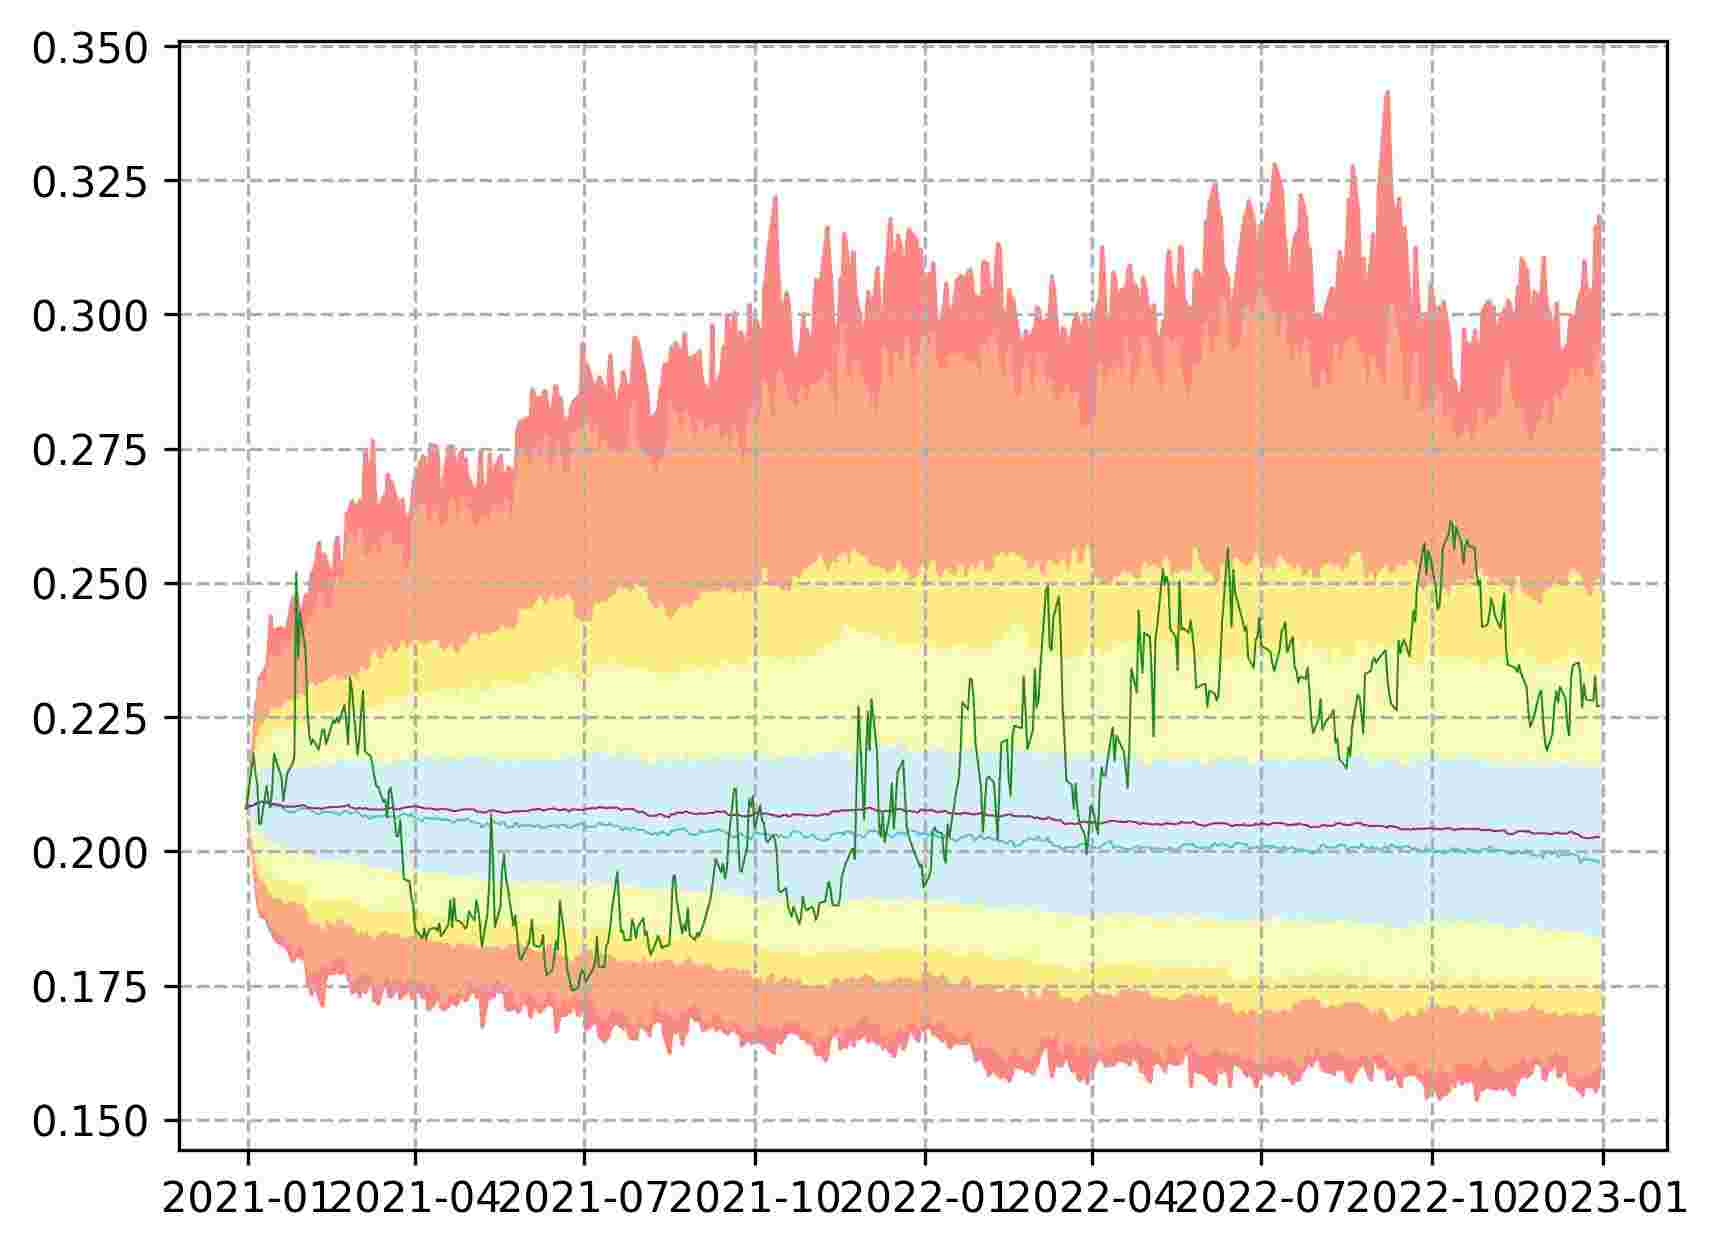
\includegraphics[width=0.25\linewidth]{SPX_ATM_12M_Out_Sample.jpg}}
    \subfigure[24-months ATM implied volatility (S\&P 500)]{ 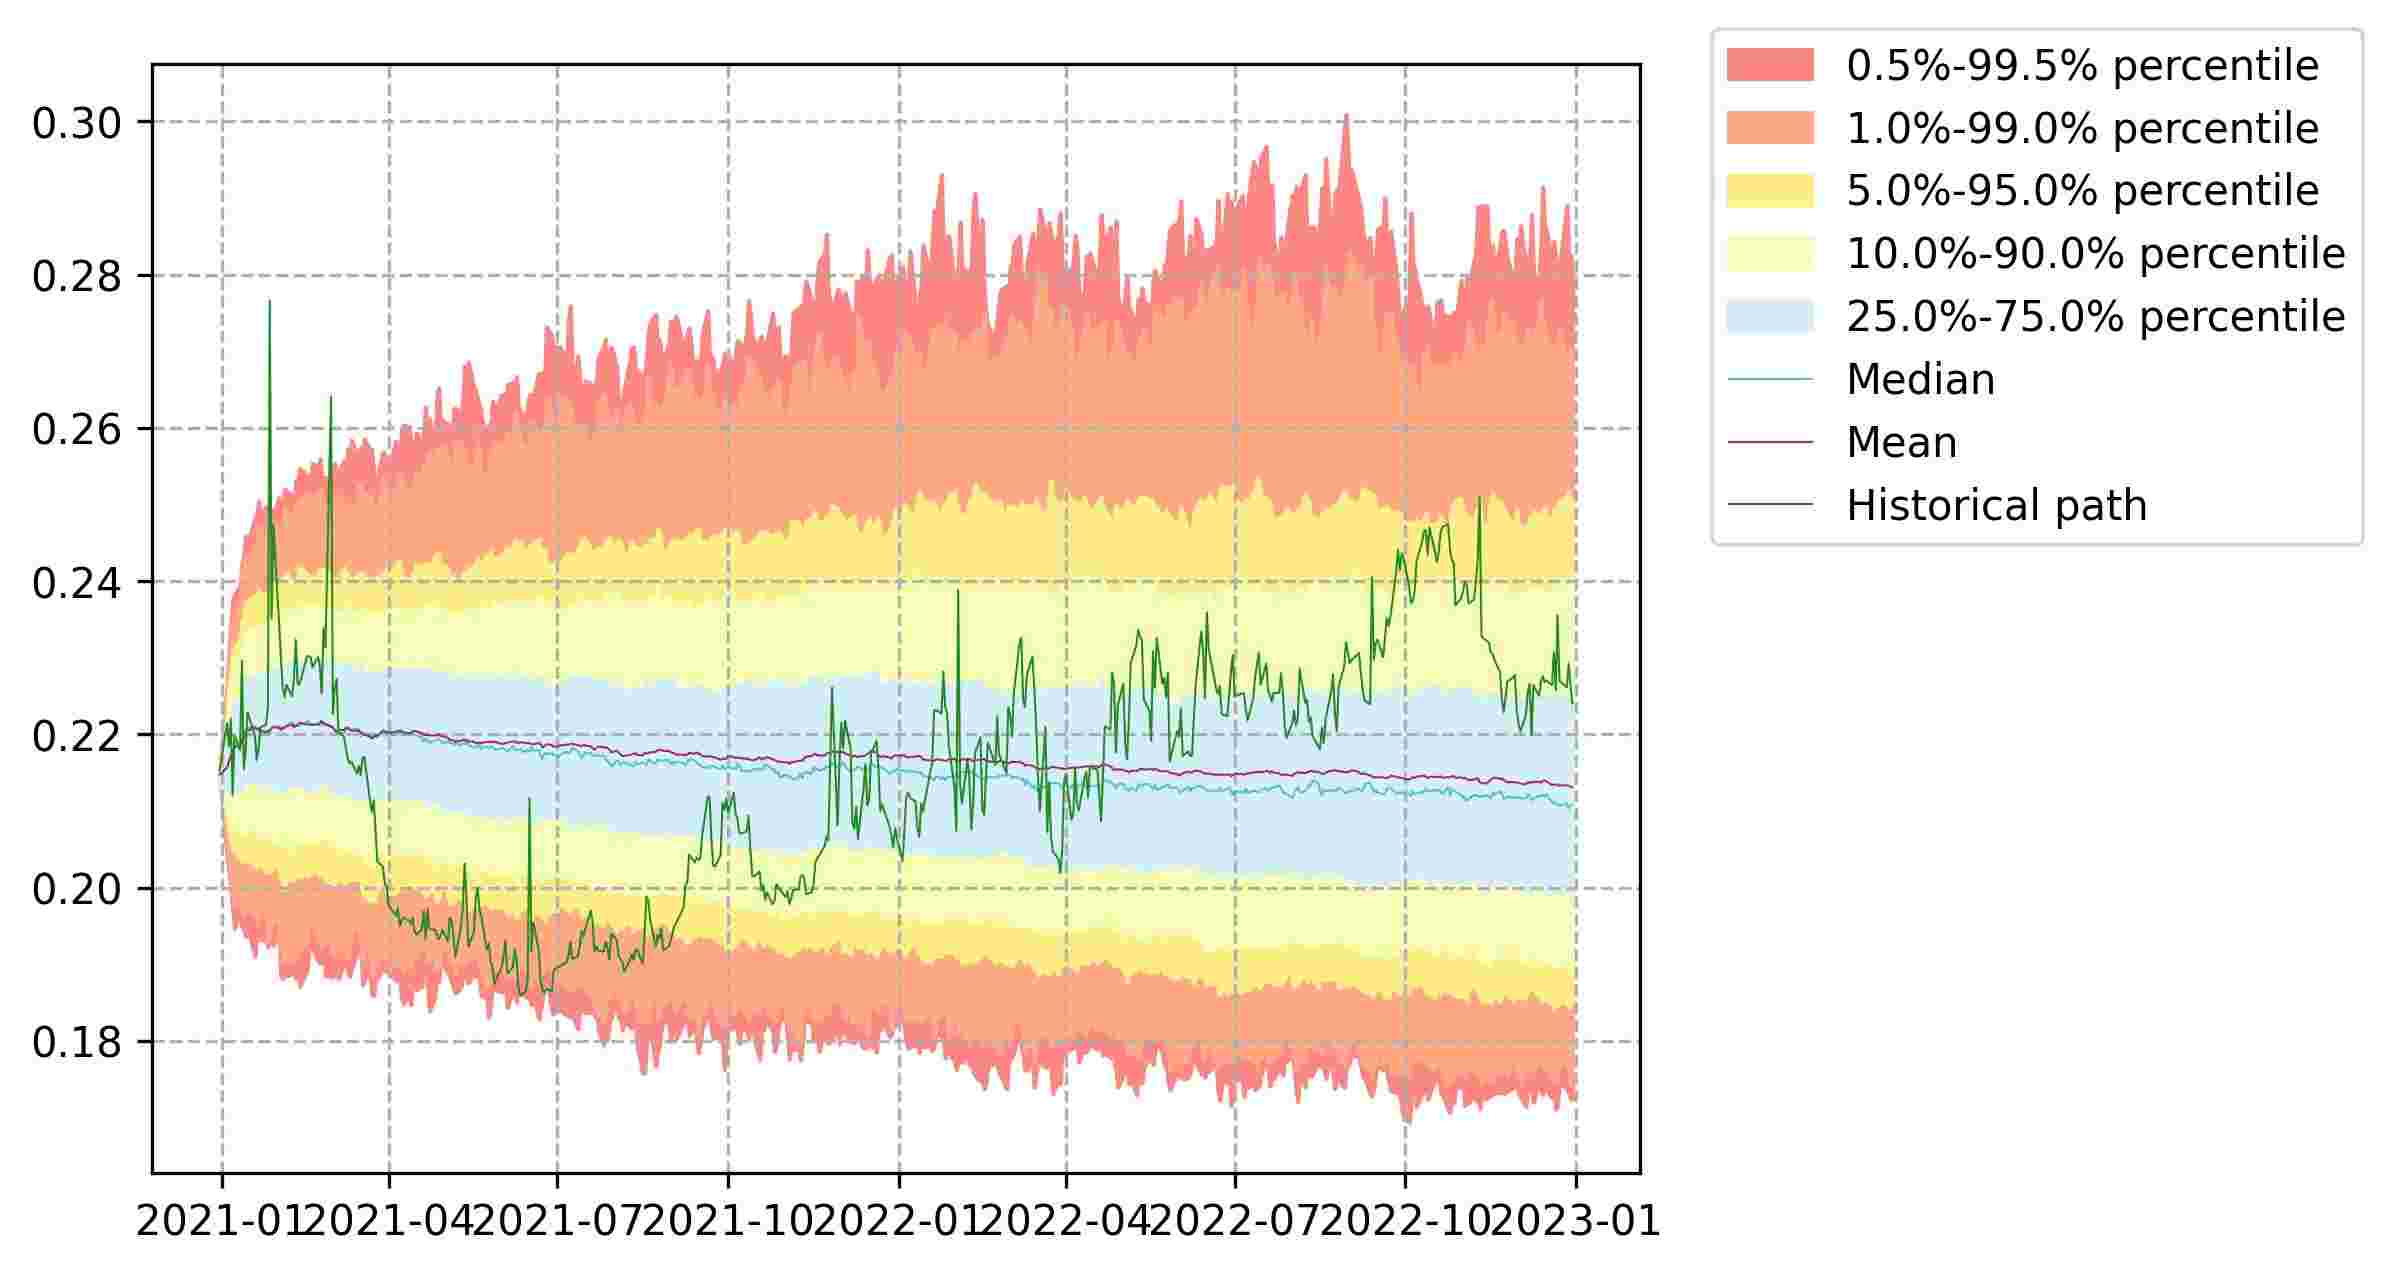
\includegraphics[width=0.36\linewidth]{SPX_ATM_24M_Out_Sample.jpg}}
    \subfigure[1-month ATM implied volatility (Euro Stoxx 50)]{ 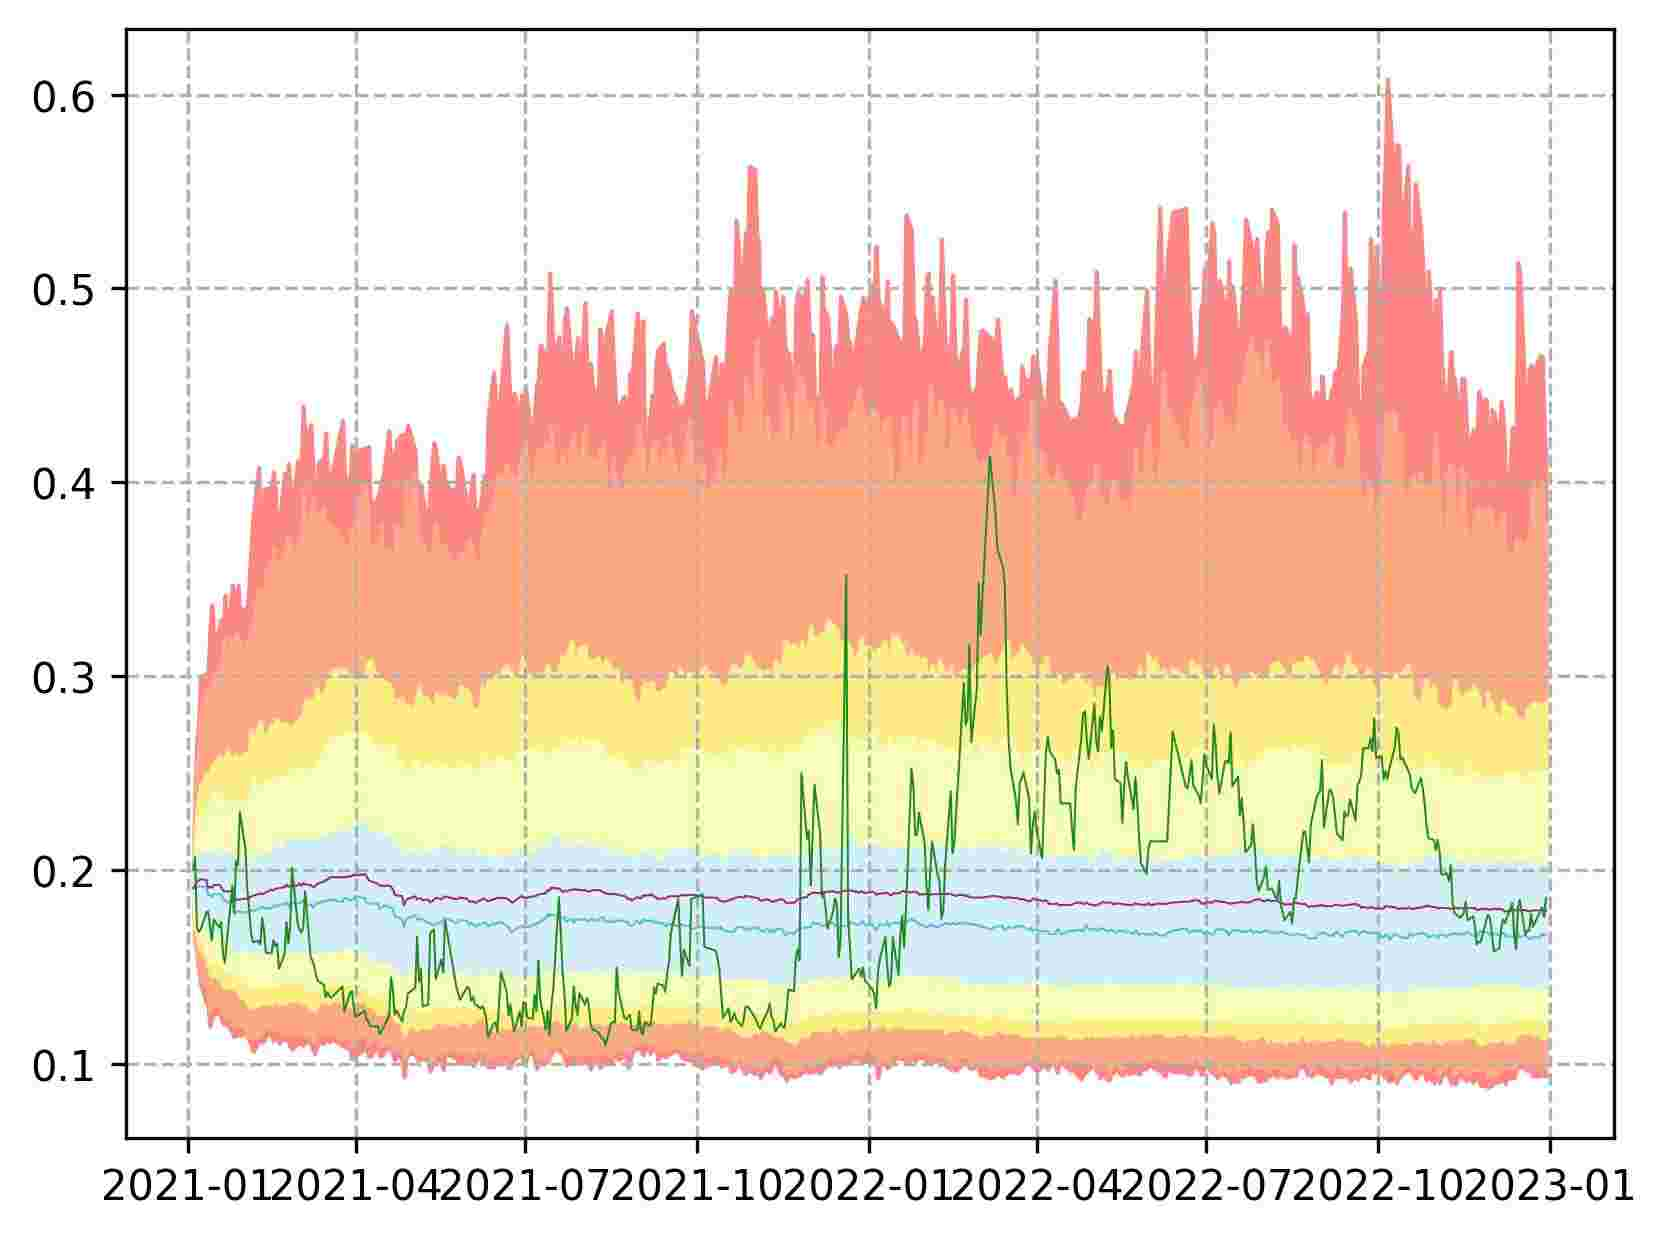
\includegraphics[width=0.25\linewidth]{STXE_ATM_1M_Out_Sample.jpg}}
    \subfigure[12-months ATM implied volatility (Euro Stoxx 50)]{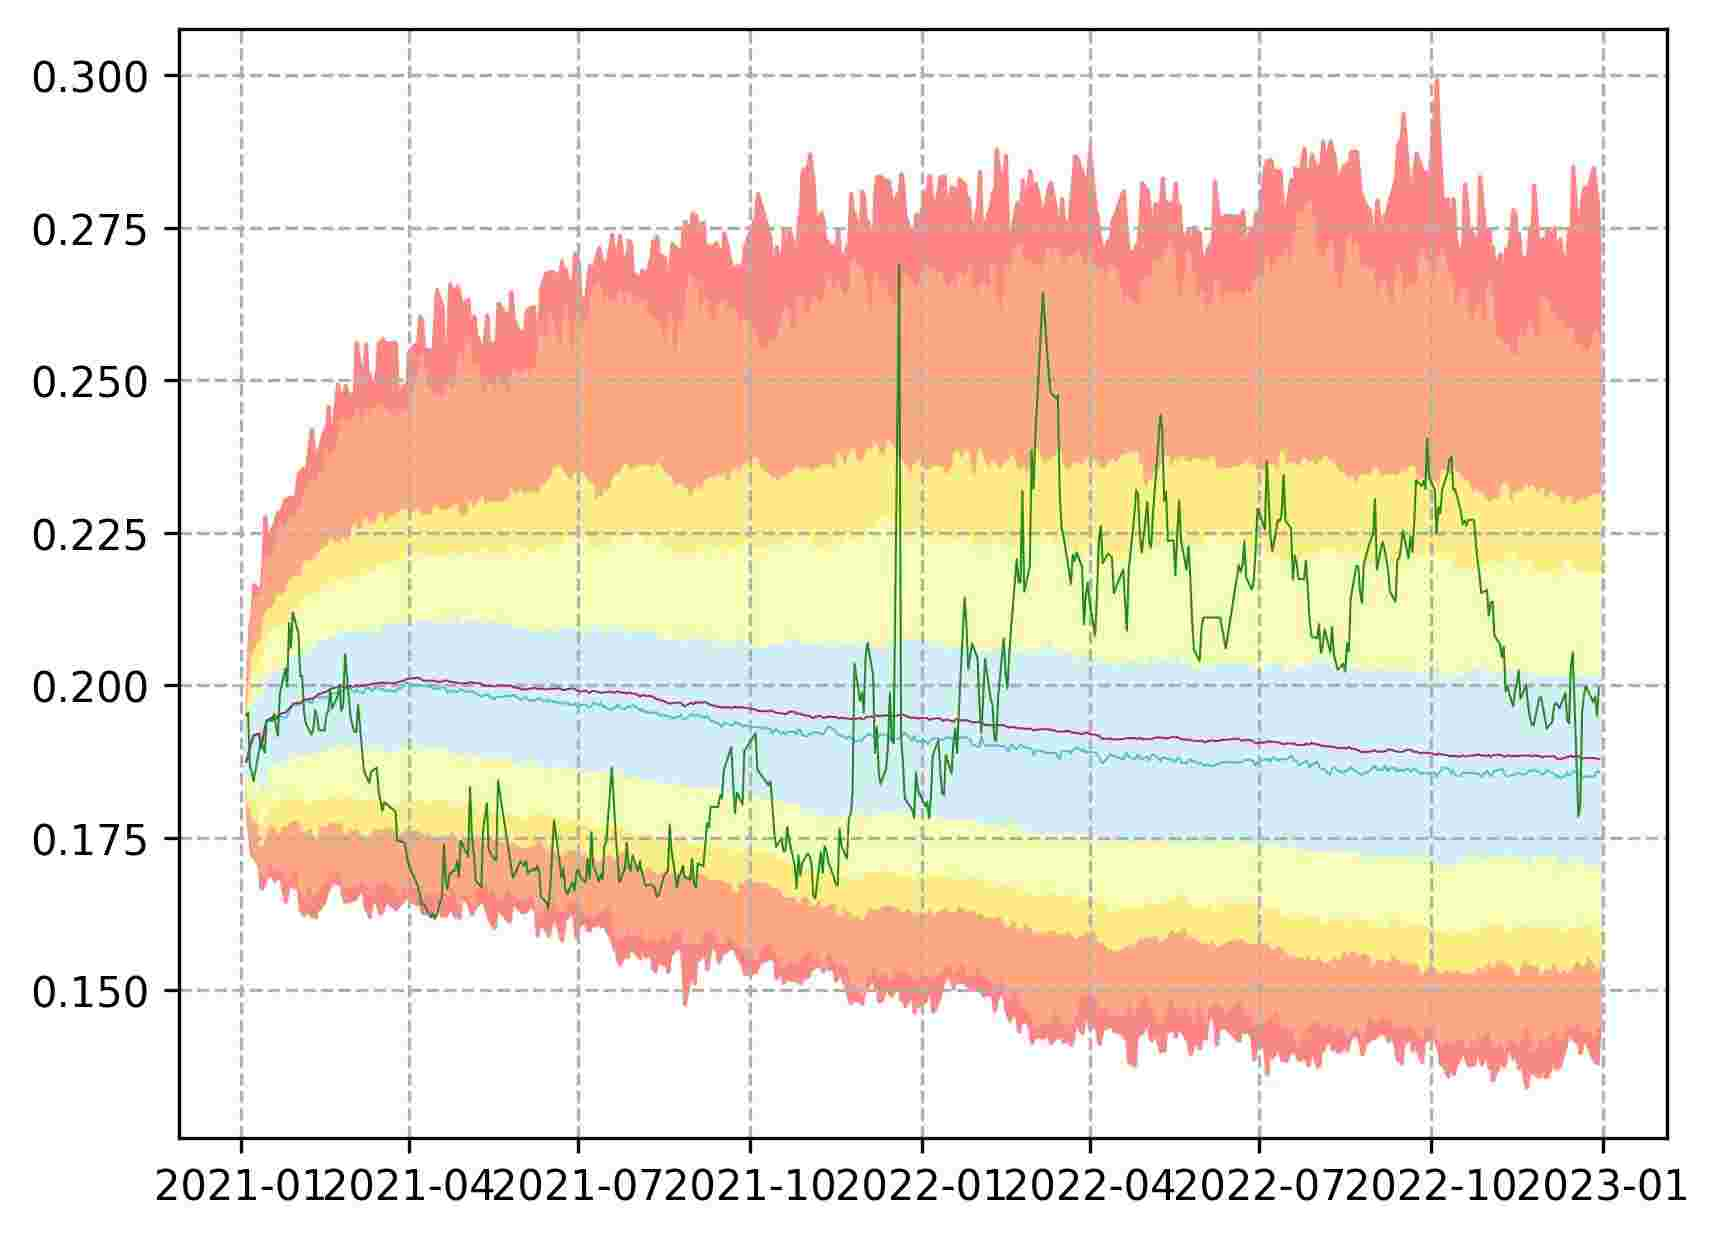
\includegraphics[width=0.25\linewidth]{STXE_ATM_12M_Out_Sample.jpg}}
    \subfigure[24-months ATM implied volatility (Euro Stoxx 50)]{ 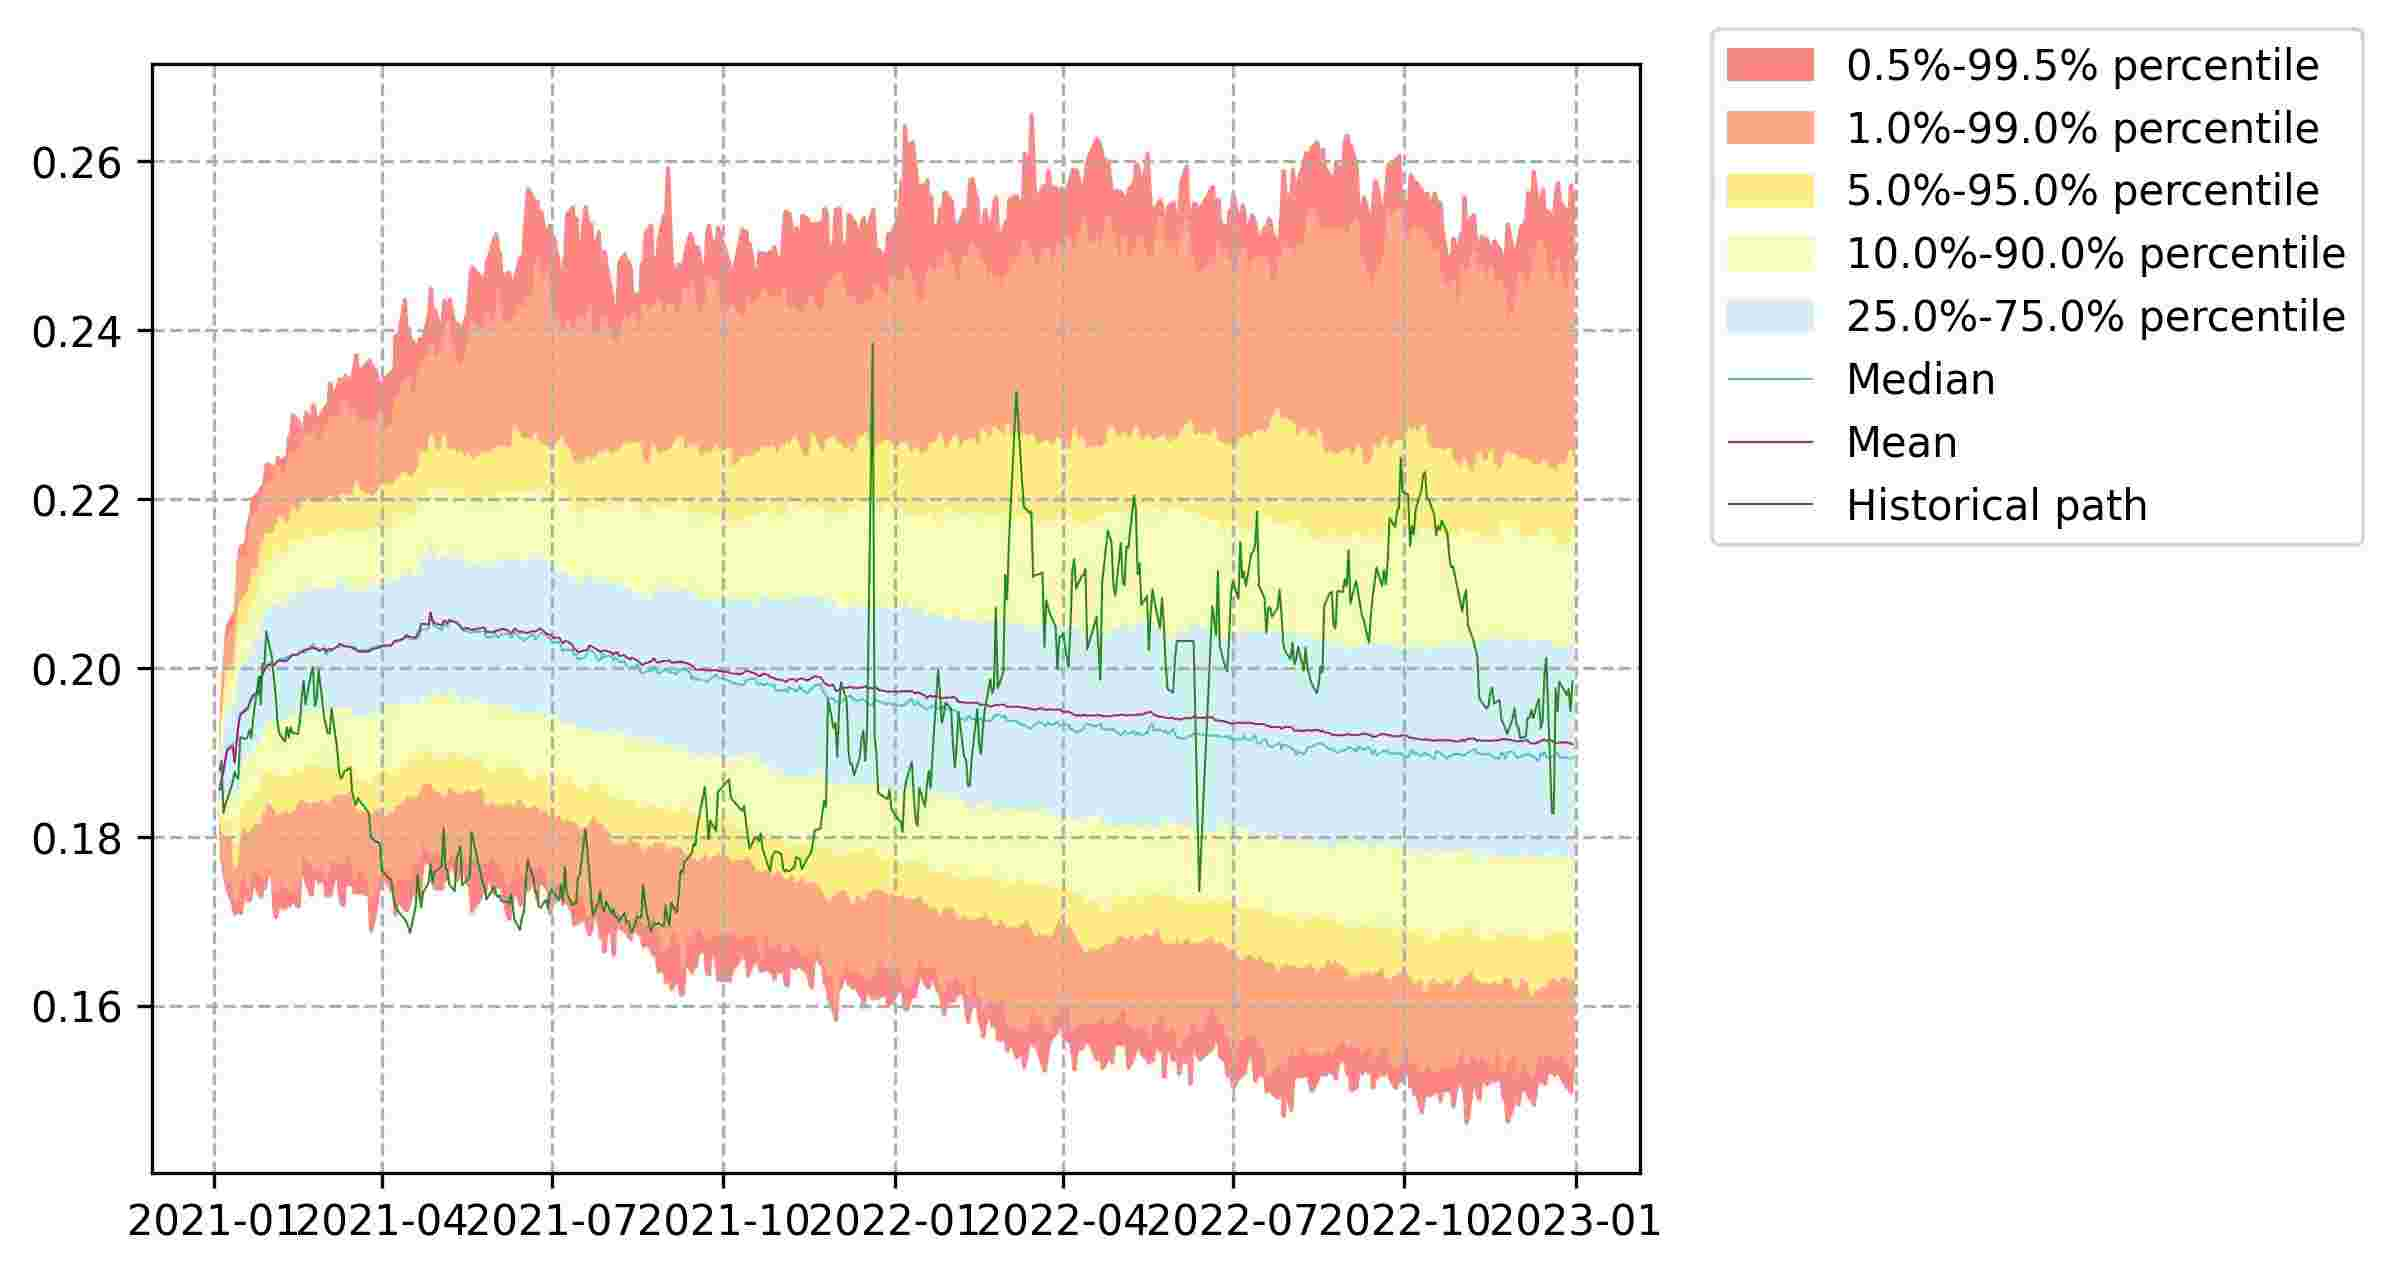
\includegraphics[width=0.36\linewidth]{STXE_ATM_24M_Out_Sample.jpg}}
    \caption{Out-of-sample quantiles envelopes of the ATM implied volatility for several time-to-maturities.}
\label{fig:quantiles_envelopes_oos}
\end{figure}

\begin{figure}
    \centering
    \subfigure[Historical average IVS of the S\&P 500 ]{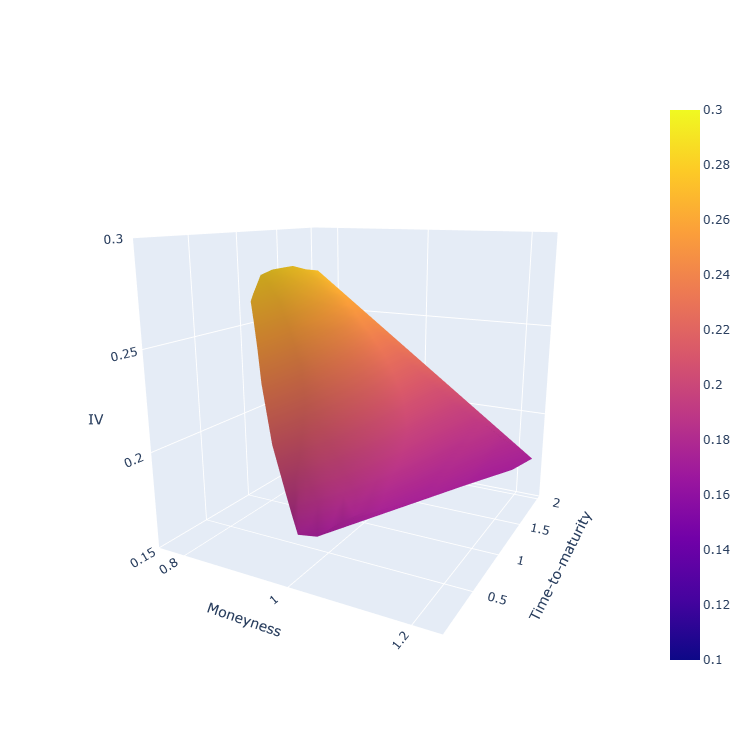
\includegraphics[width=0.45\linewidth]{SPX_Hist_Average_IV.png}}
    \subfigure[Simulated average IVS of the S\&P 500]{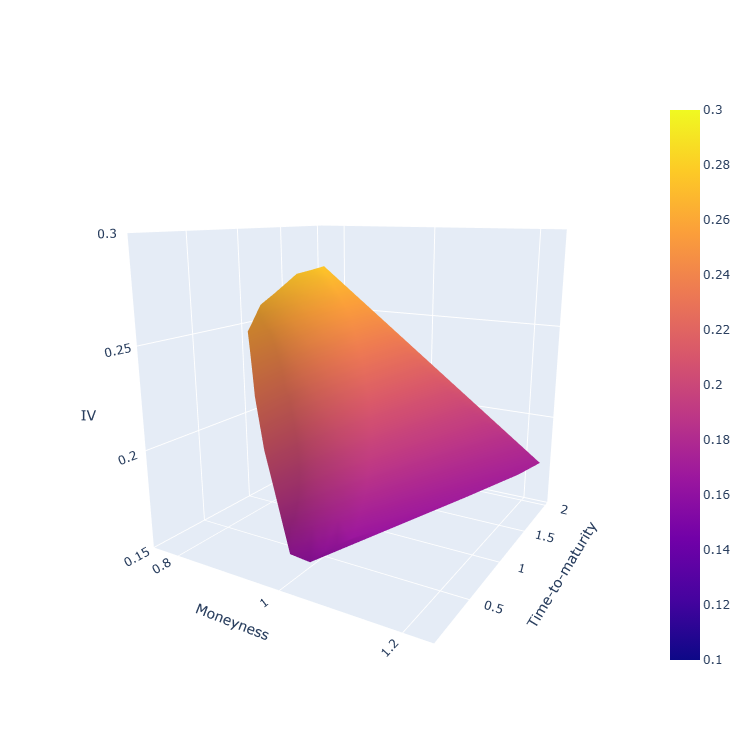
\includegraphics[width=0.45\linewidth]{SPX_Simus_Average_IV.png}}
    \subfigure[Historical average IVS of the Euro Stoxx 50 ]{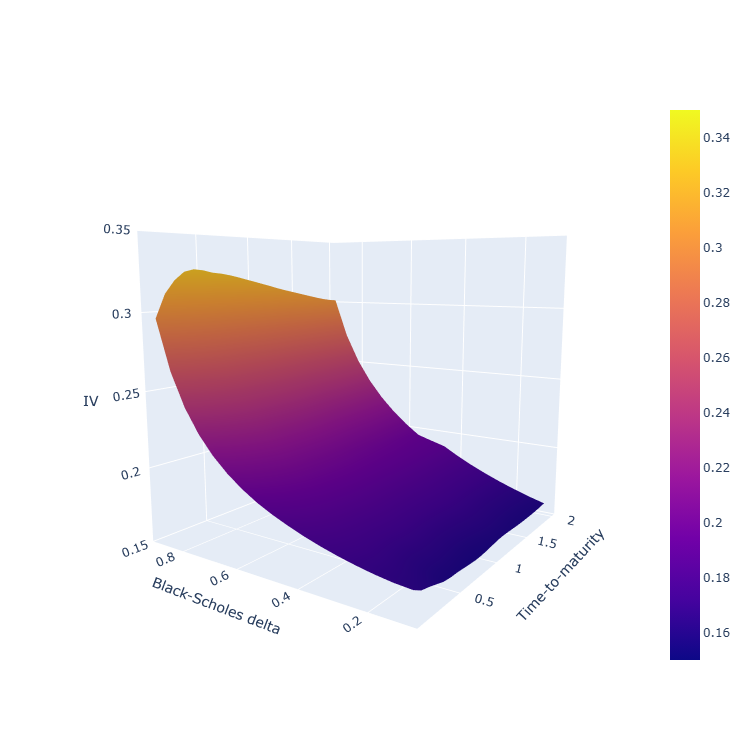
\includegraphics[width=0.45\linewidth]{STXE_Hist_Average_IV.png}}
    \subfigure[Simulated average IVS of the Euro Stoxx 50]{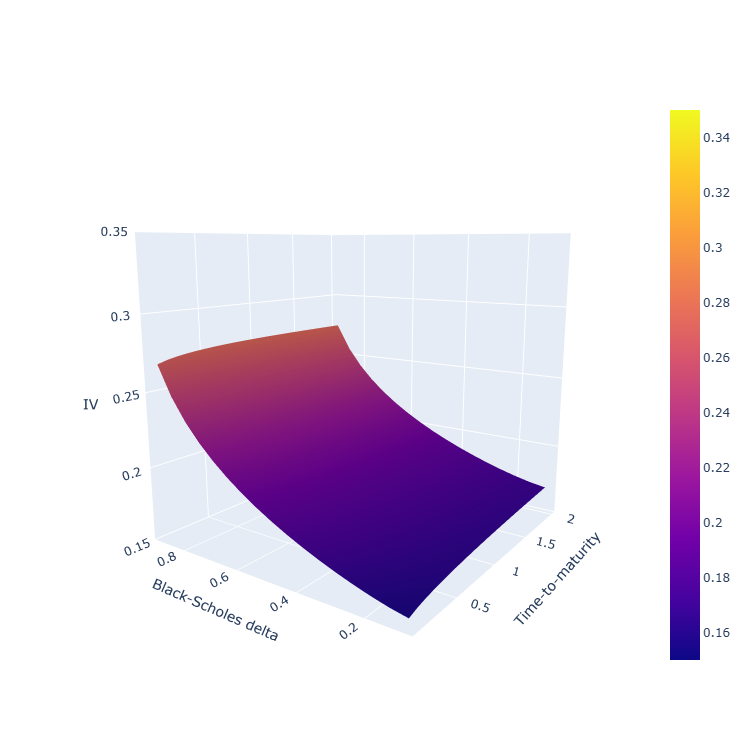
\includegraphics[width=0.45\linewidth]{STXE_Simus_Average_IV.png}}
    \caption{Comparison of the historical average IVS on the test set and the simulated average IVS. Note that the S\&P 500 IVSs are not rectangular because, for each time-to-maturity, we select the values of the moneyness for which the Black-Scholes delta of a call option is historically always between 0.1 and 0.9 (consistently with the calibration of the parsimonious SSVI parameters, see Appendix \ref{sec:ssvi_calibration_results}). On the other hand, the Euro Stoxx 50 IVS is rectangular because the options in our data set are available on a regular grid of Black-Scholes delta instead of being available on a grid of forward moneynesses (see Section \ref{sec:data}). To simulate IVSs on this Black-Scholes delta grid, we first generate the values of the parsimonious SSVI parameters $a$, $p$, $\rho$, and $\eta$. Then, using the Newton-Raphson method, we find the moneynesses such that the Black-Scholes deltas, calculated with the simulated SSVI volatility, match those in our Black-Scholes delta grid.}
\label{fig:average_ivs}
\end{figure}

So far, we have only focused on the distribution of the implied volatility. Since the proposed model allows jointly simulating the implied volatility and the underlying asset price, we propose to study their joint distribution. For this purpose, we use the calibrated PDV parameters of Section \ref{sec:overall_perf} for the 1 month, 12 months and 24 months time-to-maturities, and we plot the density of the pair $(\beta_0+\beta_1R_{1}+\beta_2\Sigma,IV)$ where the features $R_1$ and $\Sigma$ are computed using the simulated returns of the asset price $S$ only and $IV$ is the simulated ATM implied volatility for a given time-to-maturity. This density is compared to the points with coordinates $(\beta_0+\beta_1R_{1}+\beta_2\Sigma,IV)$ where the features $R_1$ and $\Sigma$ are computed using the historical returns of the asset price only and $IV$ is the historical ATM implied volatility for a given time-to-maturity on the test set. The results are displayed in Figure \ref{fig:kde_plots}. Despite the fact that we do not model each ATM implied volatility directly using a PDV model (which is a natural idea in view of the results presented in the empirical study of Section \ref{sec:empirical_study}), we observe that linear relationship between the ATM implied volatility and $\beta_0+\beta_1R_1+\beta_2\Sigma$ is preserved by our model (which only assumes that the parameters $a$ and $p$ are specified using a PDV model). This figure also shows that the simulated dynamics of the asset price (captured through the trend feature $R_1$ and the volatility feature $\Sigma$) is quite consistent with the historical ones. \\


\begin{figure}
    \centering
    \subfigure[1-month ATM implied volatility (S\&P 500)]{ 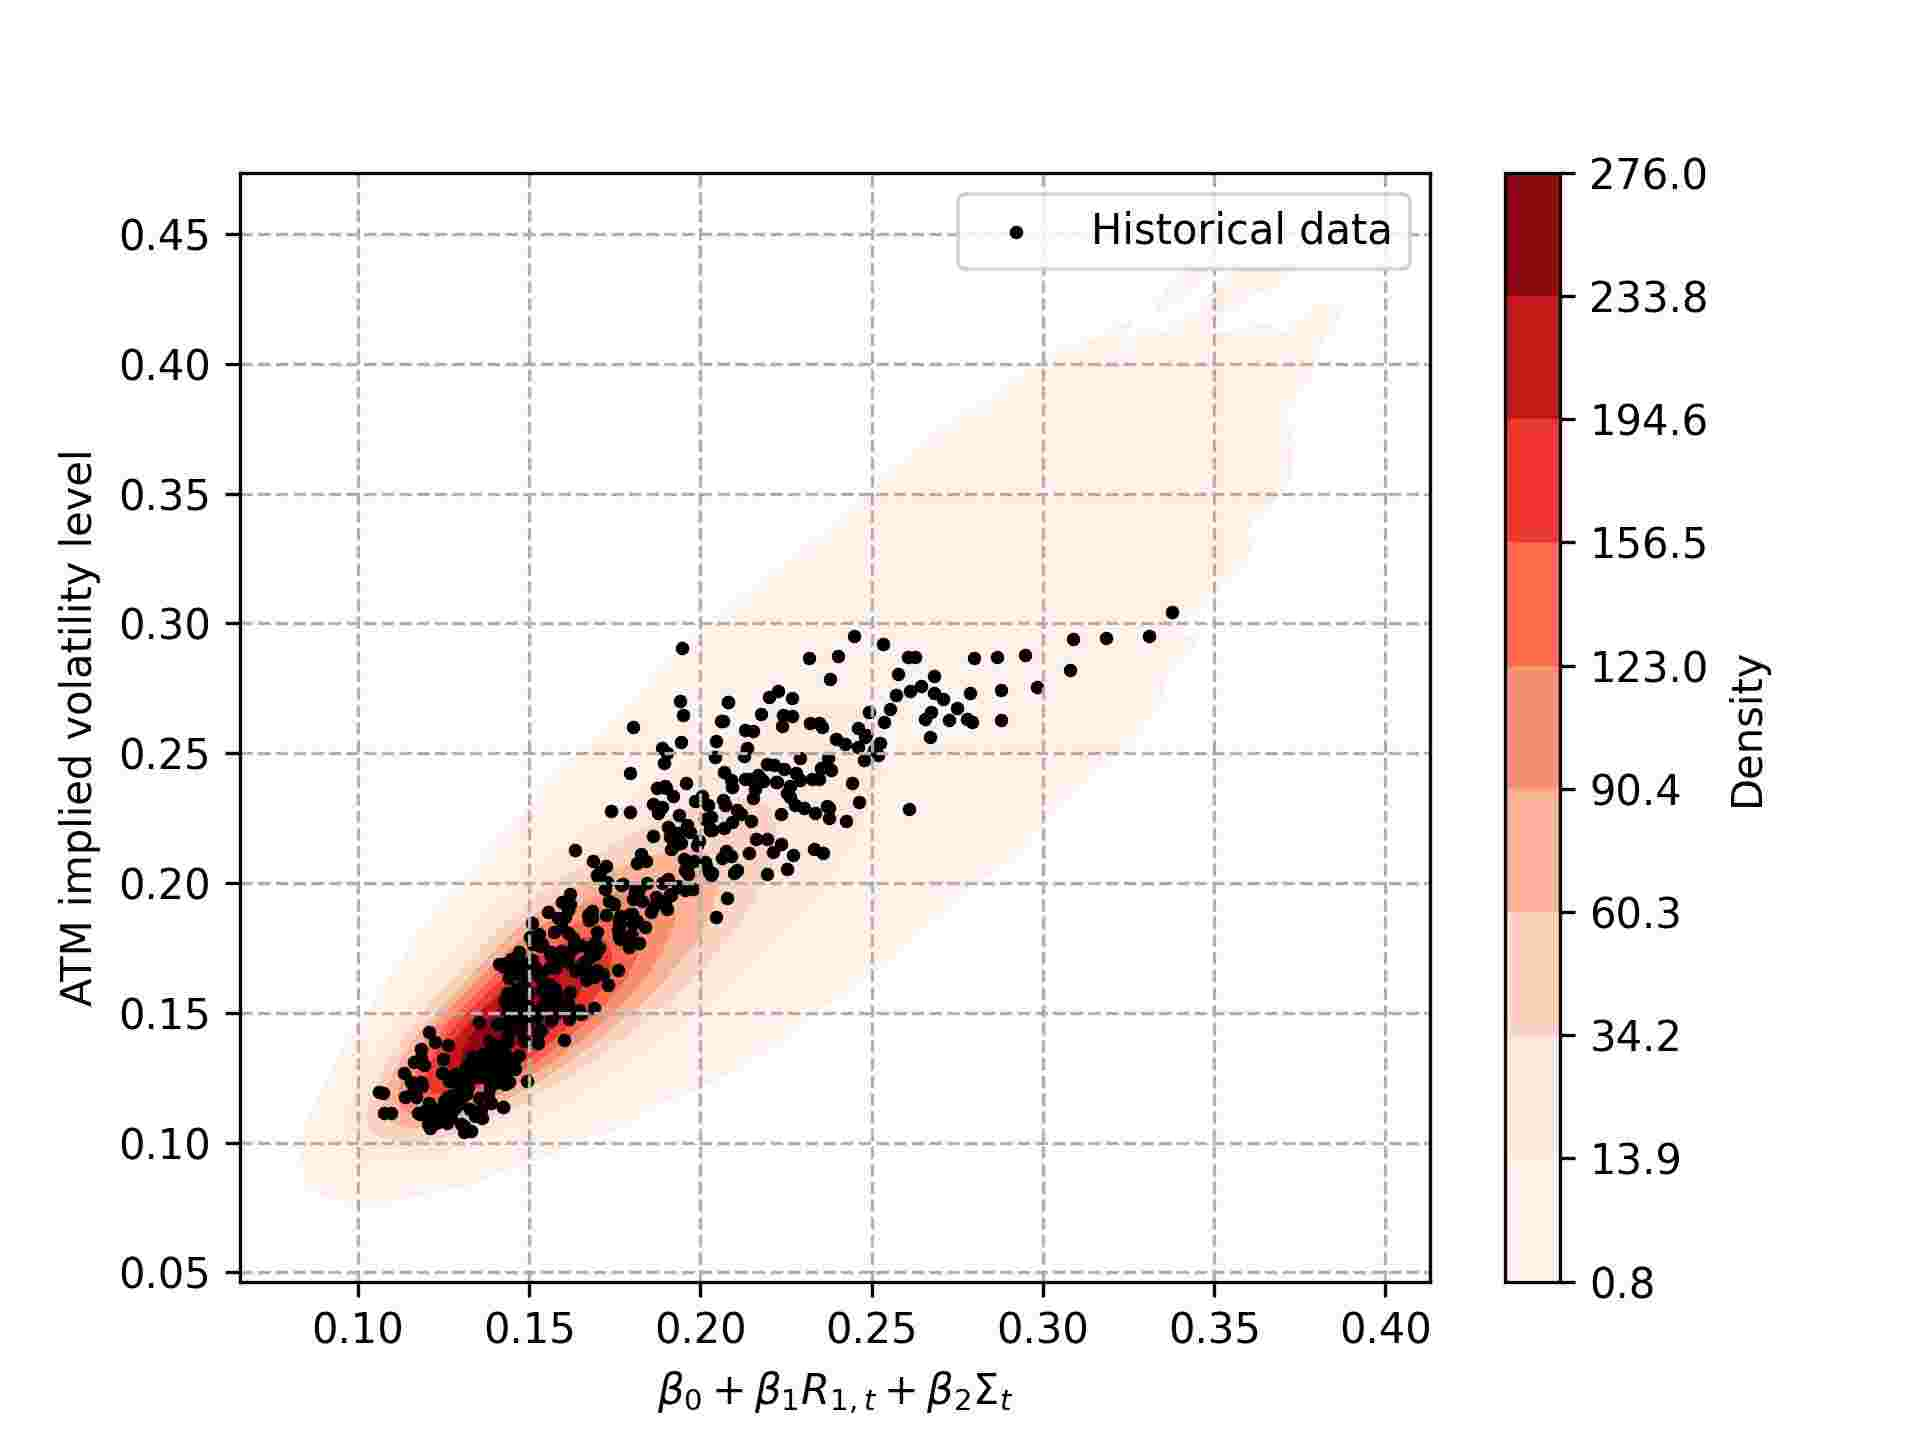
\includegraphics[width=0.3\linewidth]{SPX_KDEPlot_1M_Jacobi_Drift.jpg}}
    \subfigure[12-months ATM implied volatility (S\&P 500)]{ 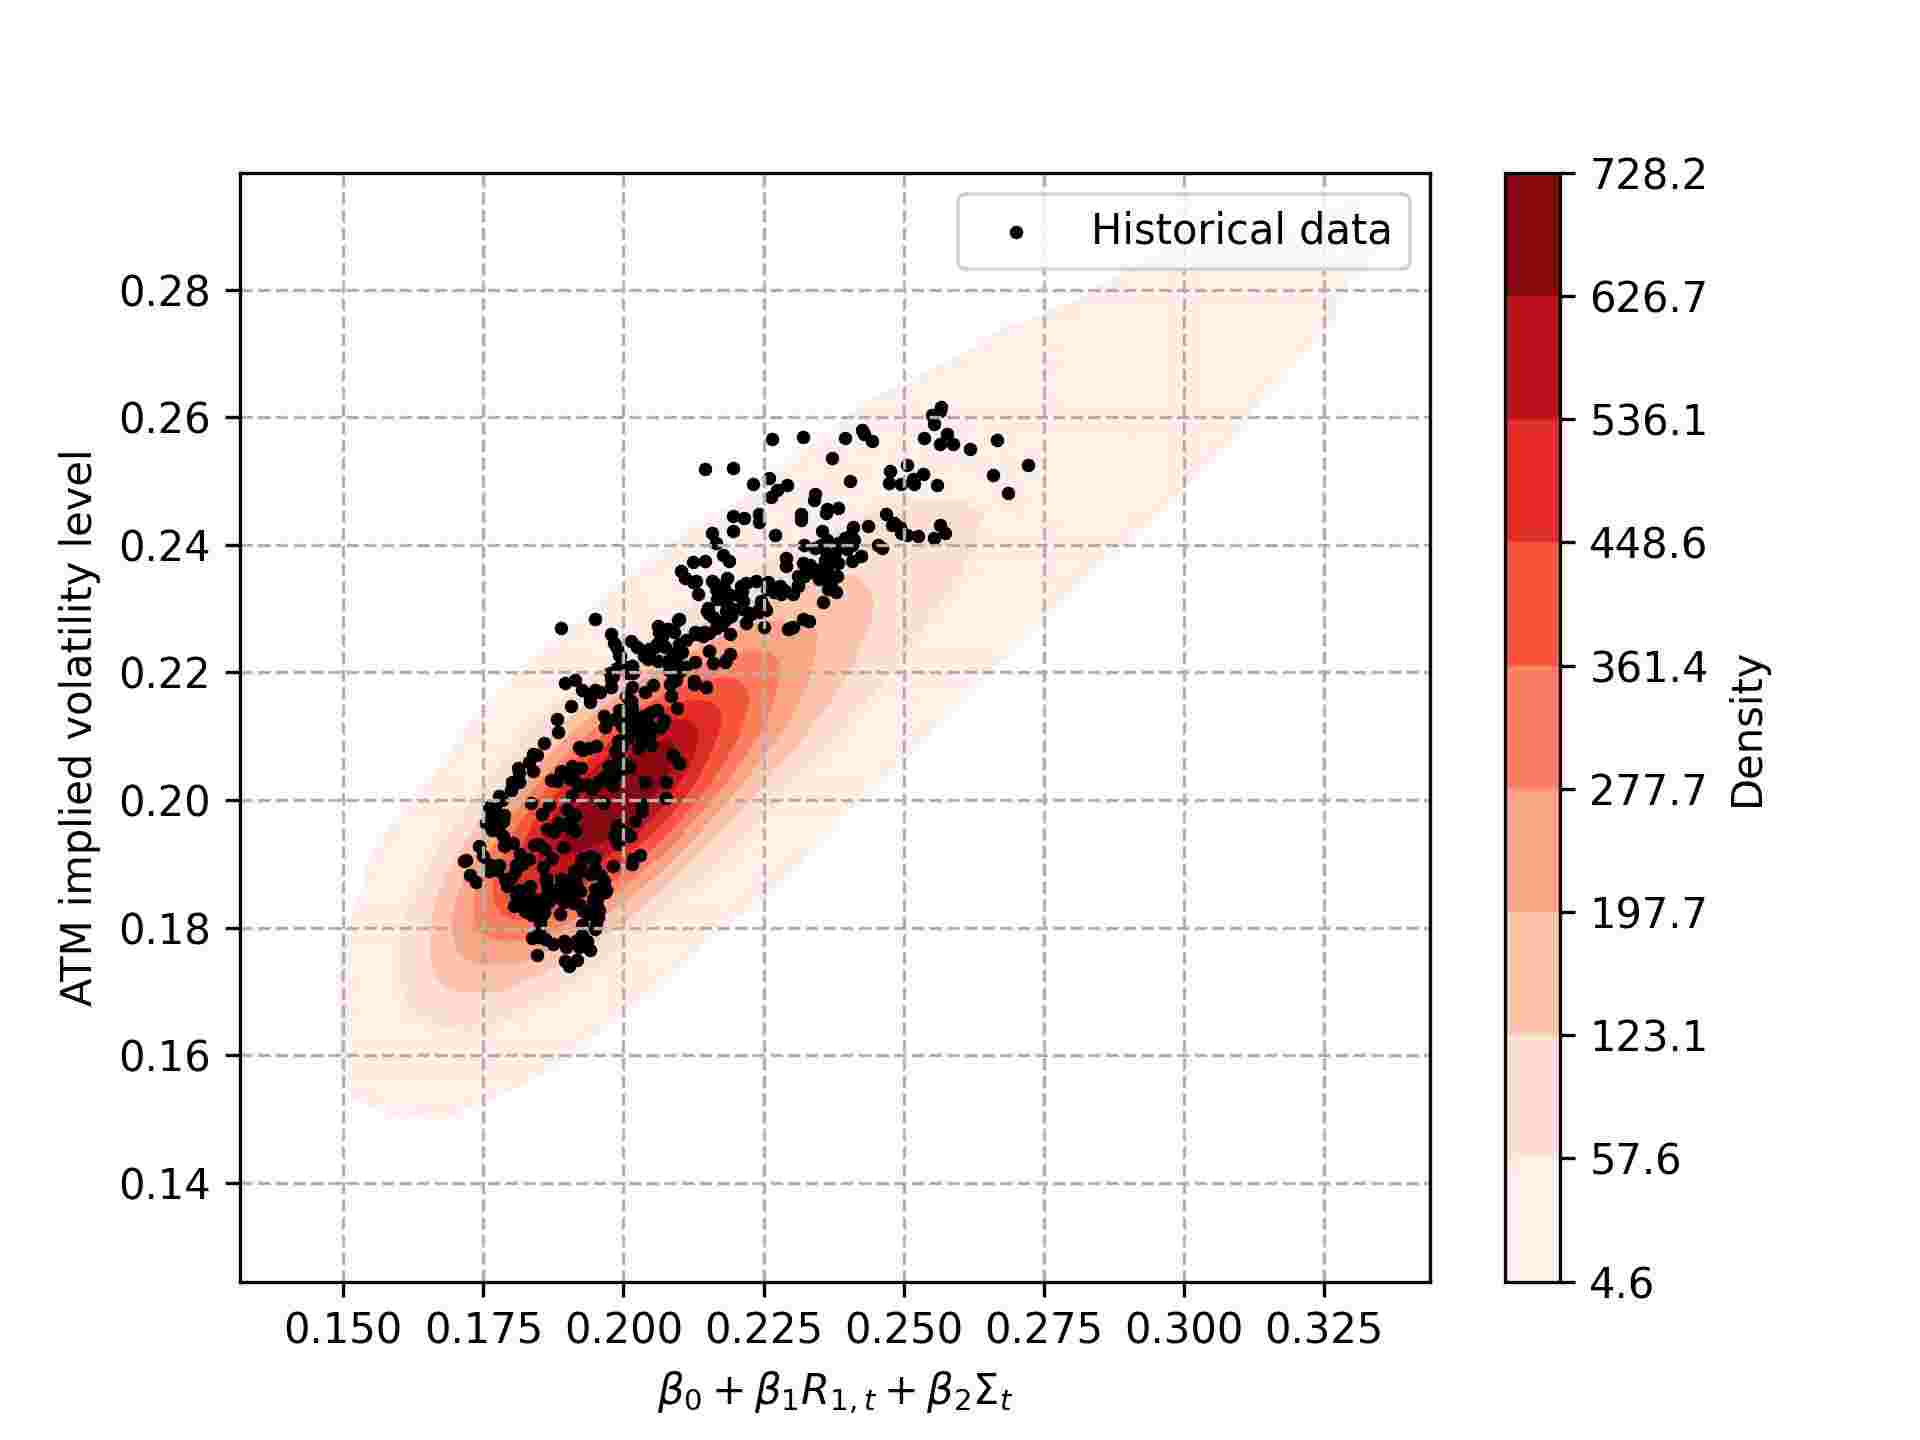
\includegraphics[width=0.3\linewidth]{SPX_KDEPlot_12M_Jacobi_Drift.jpg}}
    \subfigure[24-months ATM implied volatility (S\&P 500)]{ 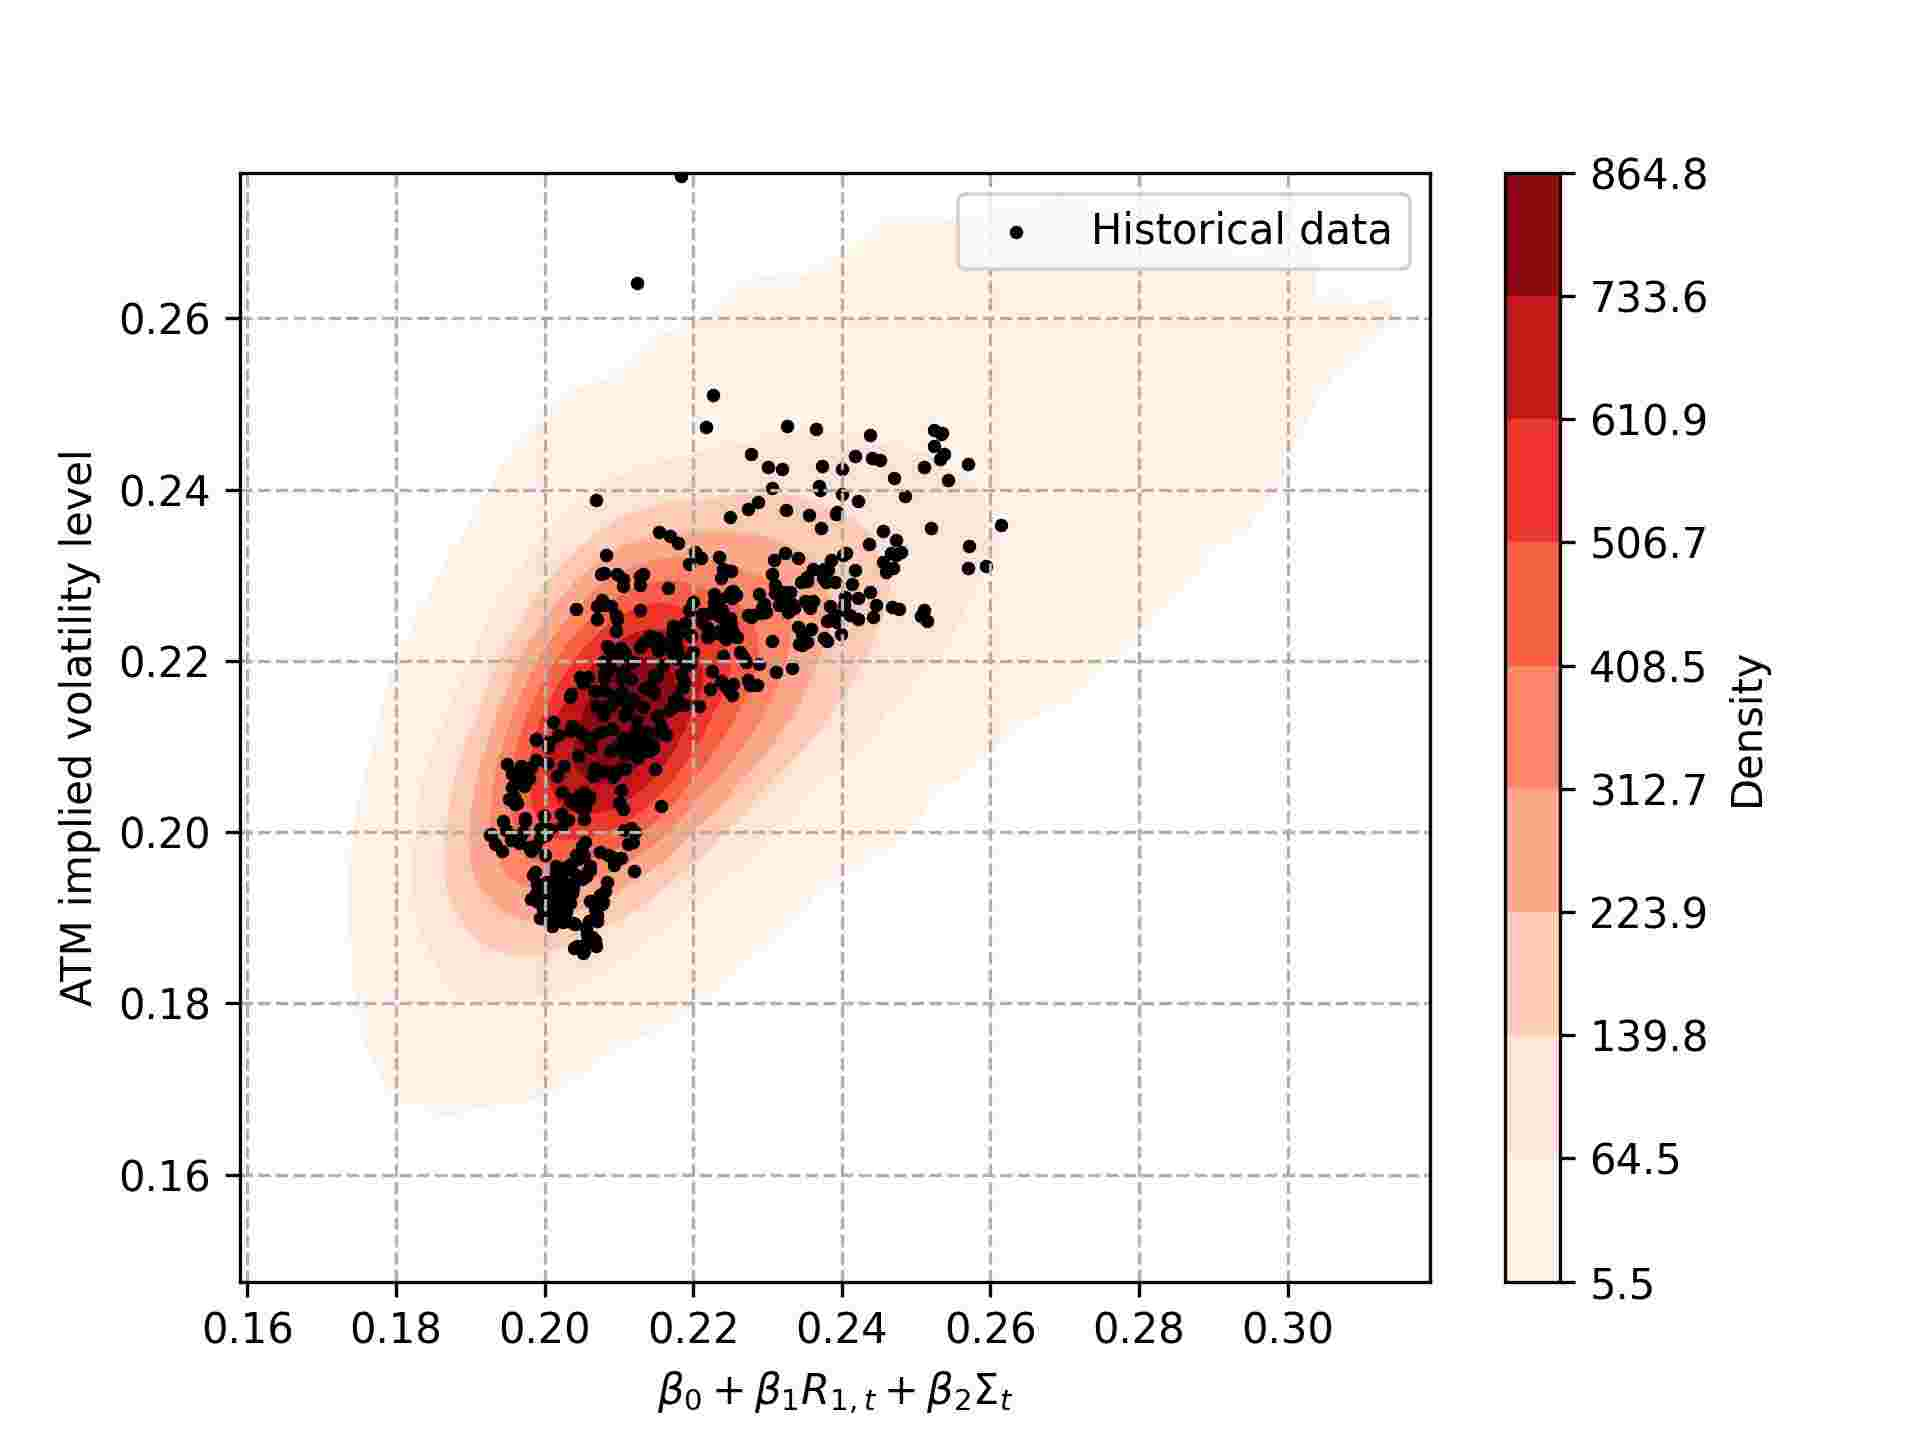
\includegraphics[width=0.3\linewidth]{SPX_KDEPlot_24M_Jacobi_Drift.jpg}}
    \subfigure[1-month ATM implied volatility (Euro Stoxx 50)]{ 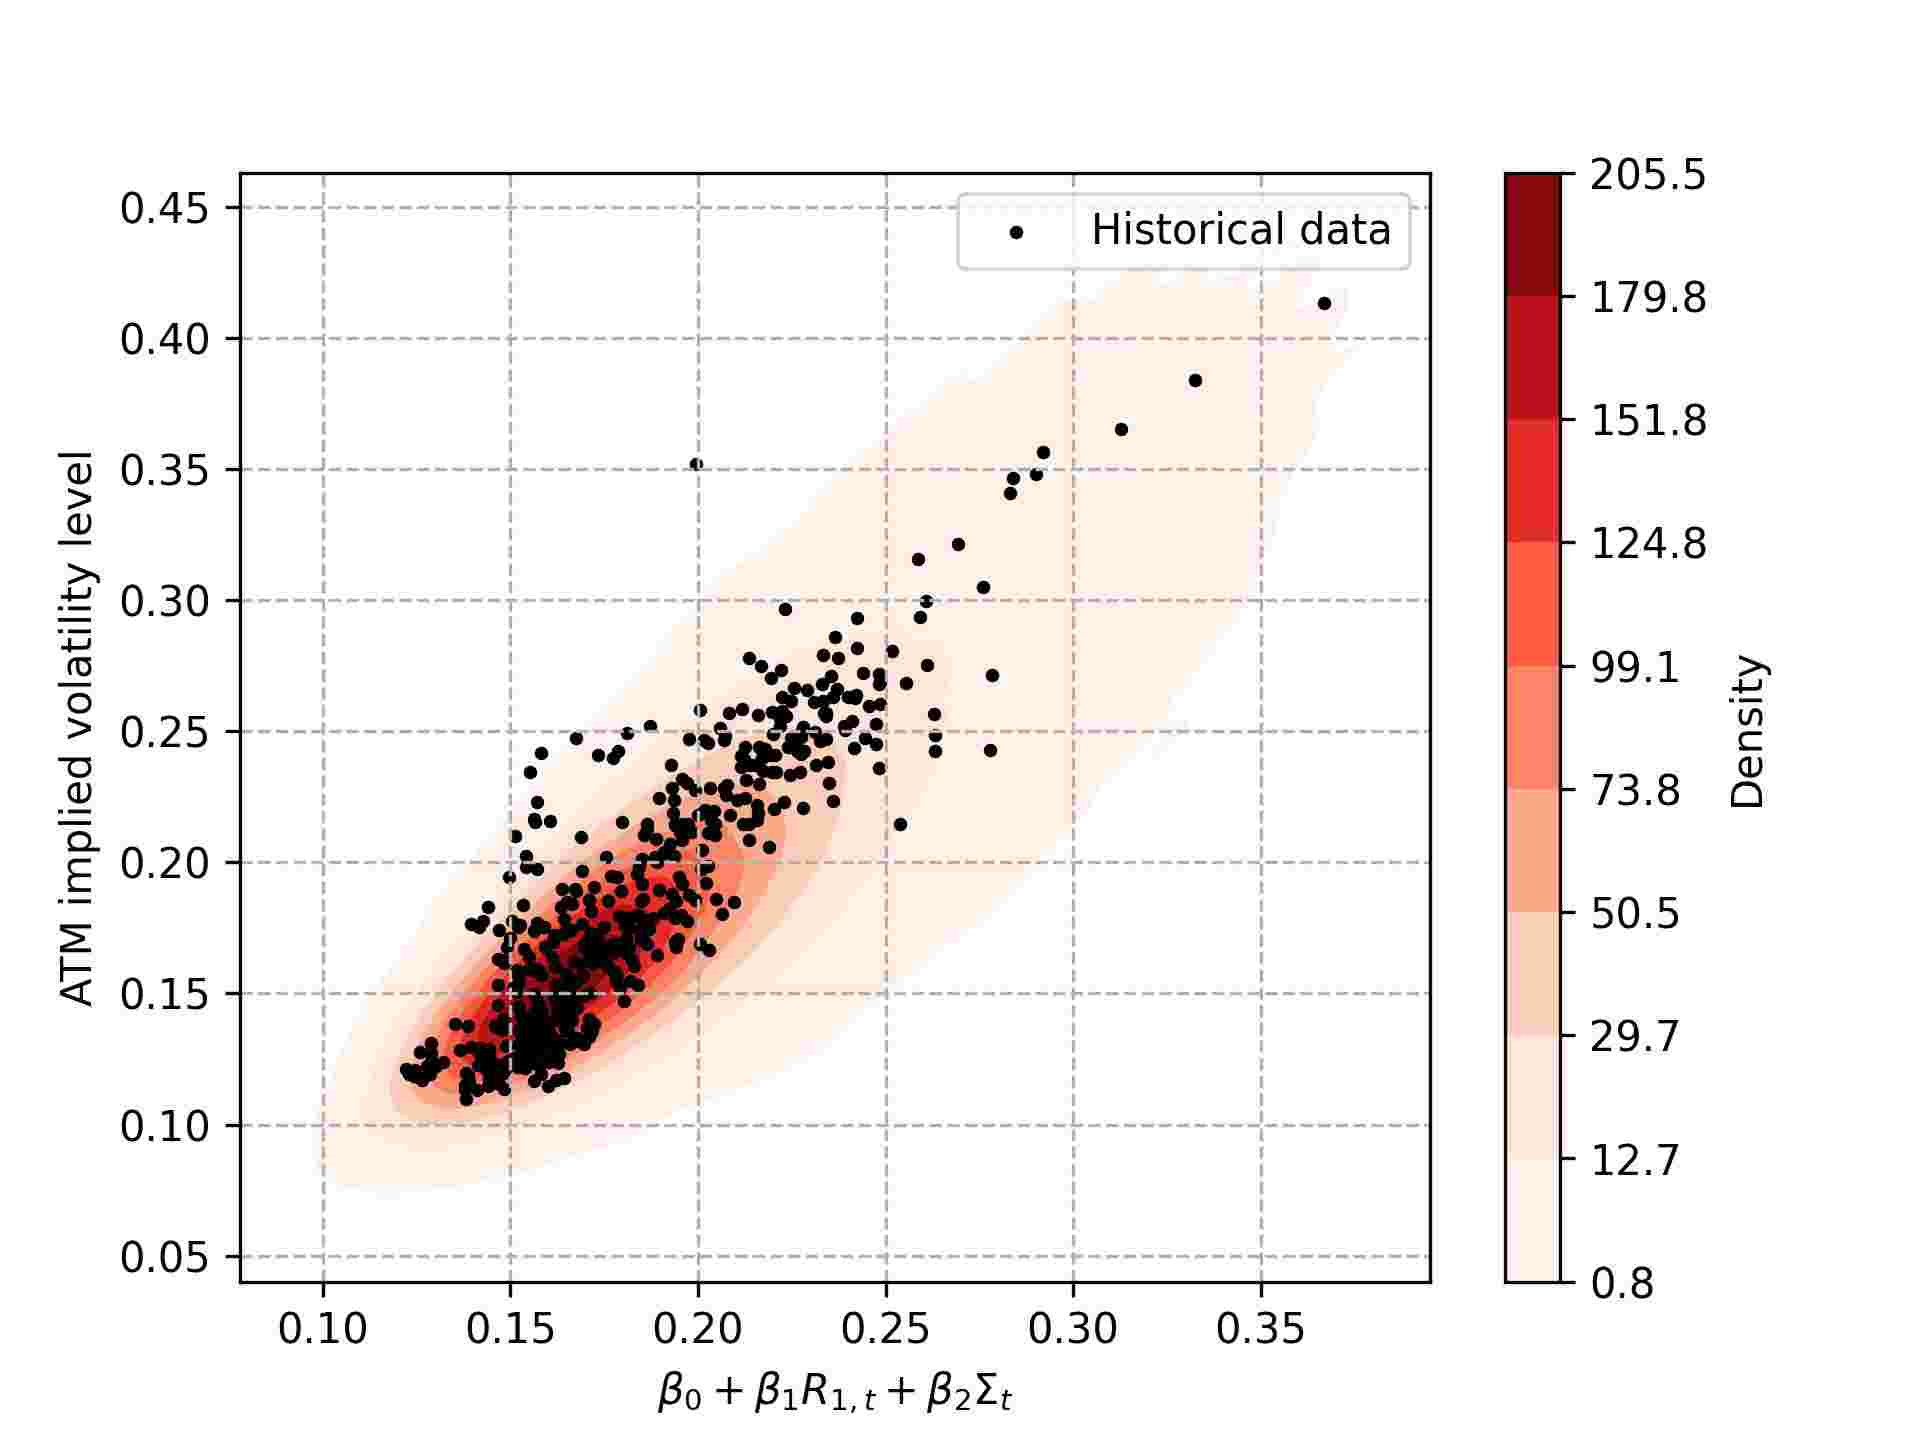
\includegraphics[width=0.3\linewidth]{STXE_KDEPlot_1M_Jacobi_Drift.jpg}}
    \subfigure[12-months ATM implied volatility (Euro Stoxx 50)]{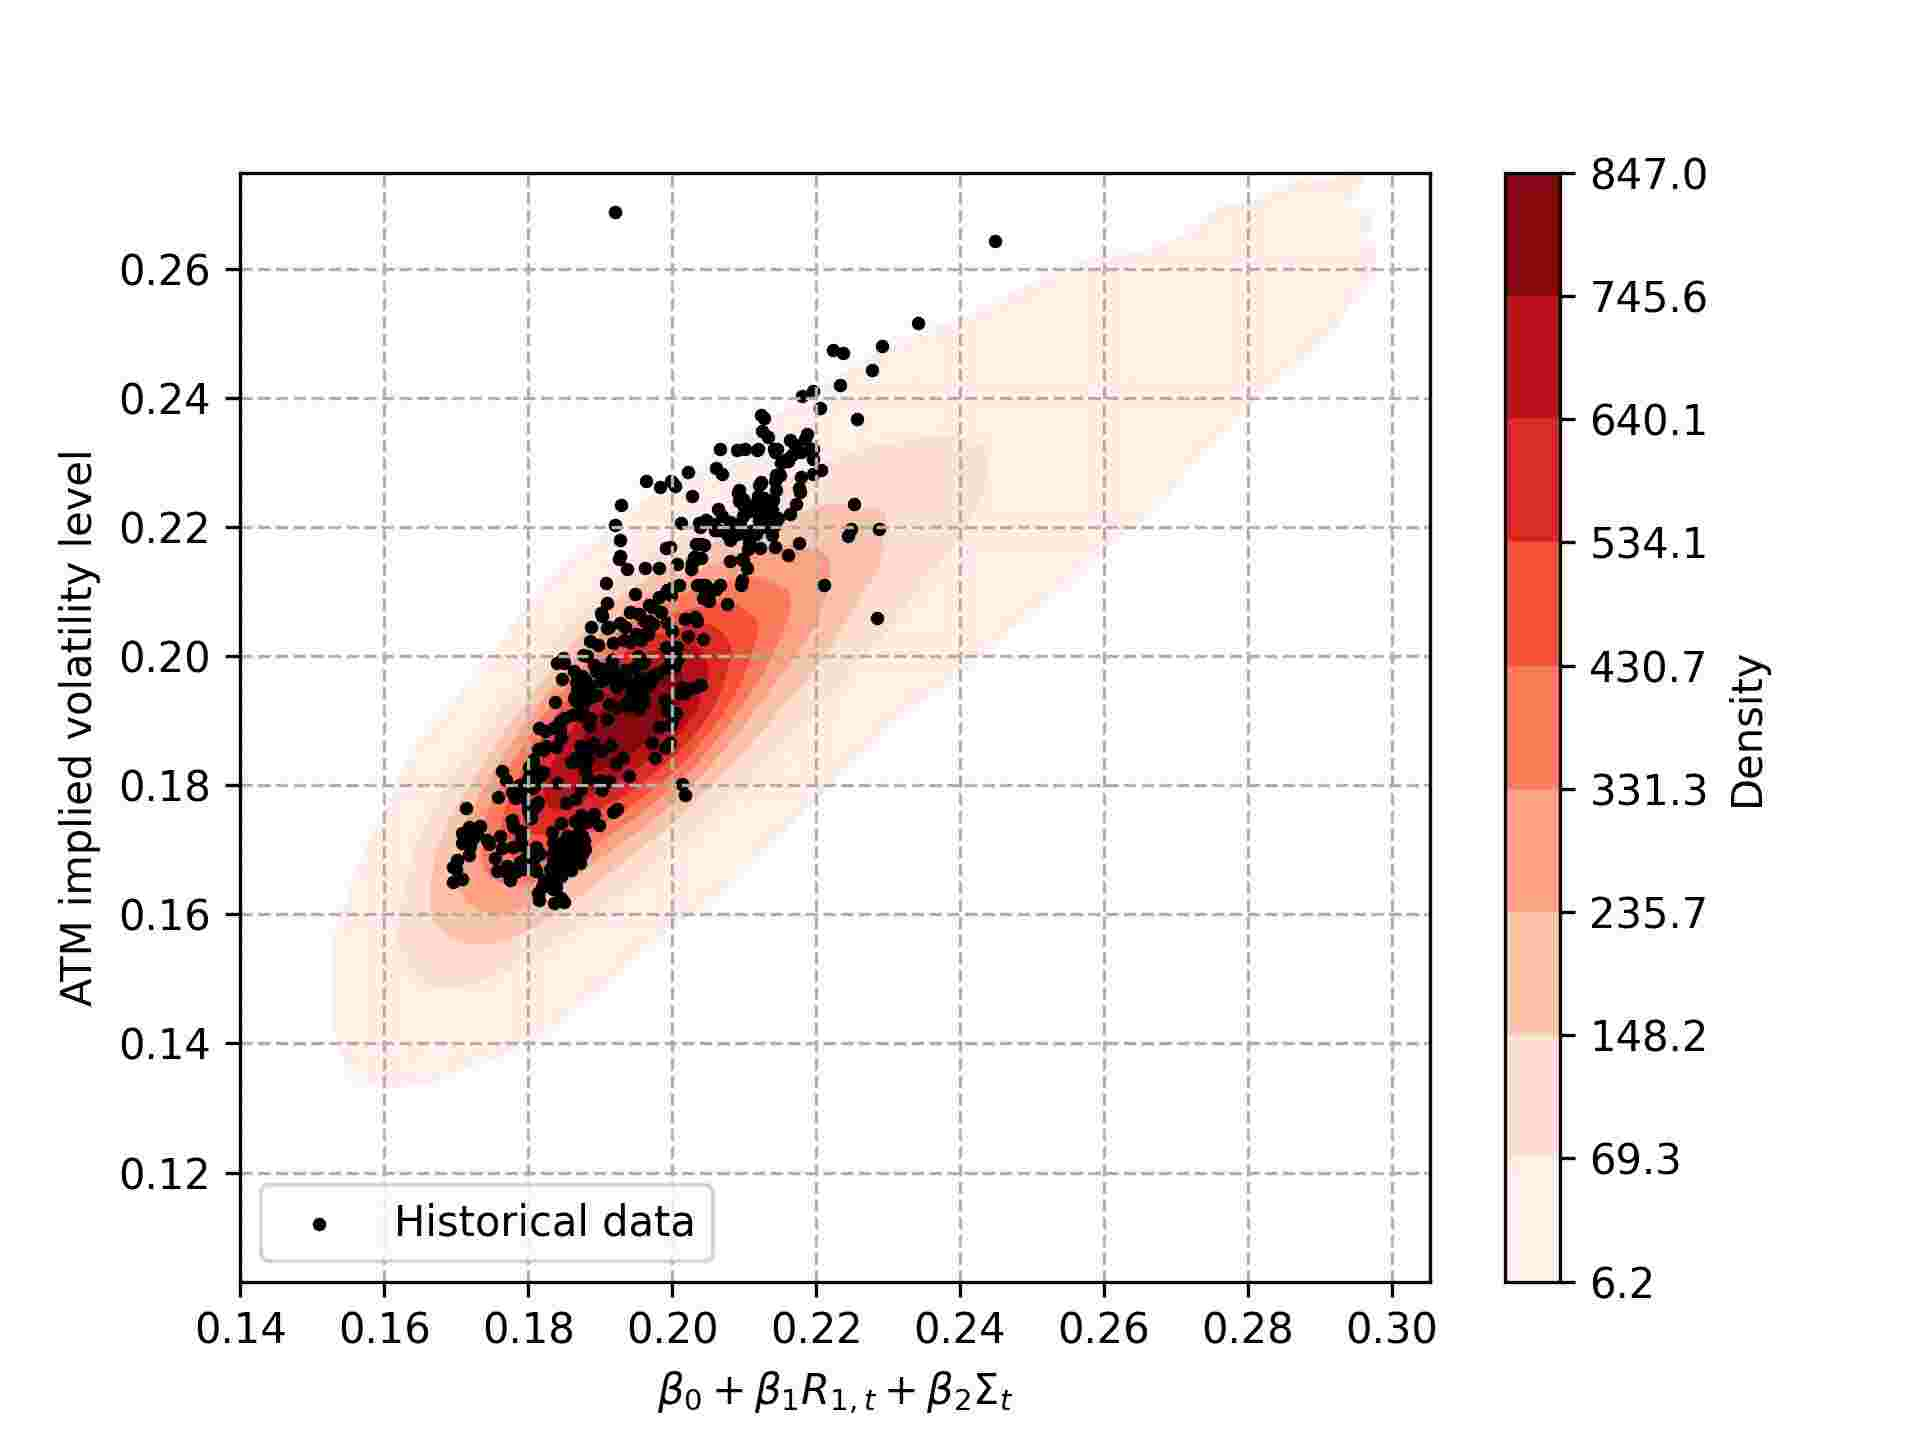
\includegraphics[width=0.3\linewidth]{STXE_KDEPlot_12M_Jacobi_Drift.jpg}}
    \subfigure[24-months ATM implied volatility (Euro Stoxx 50)]{ 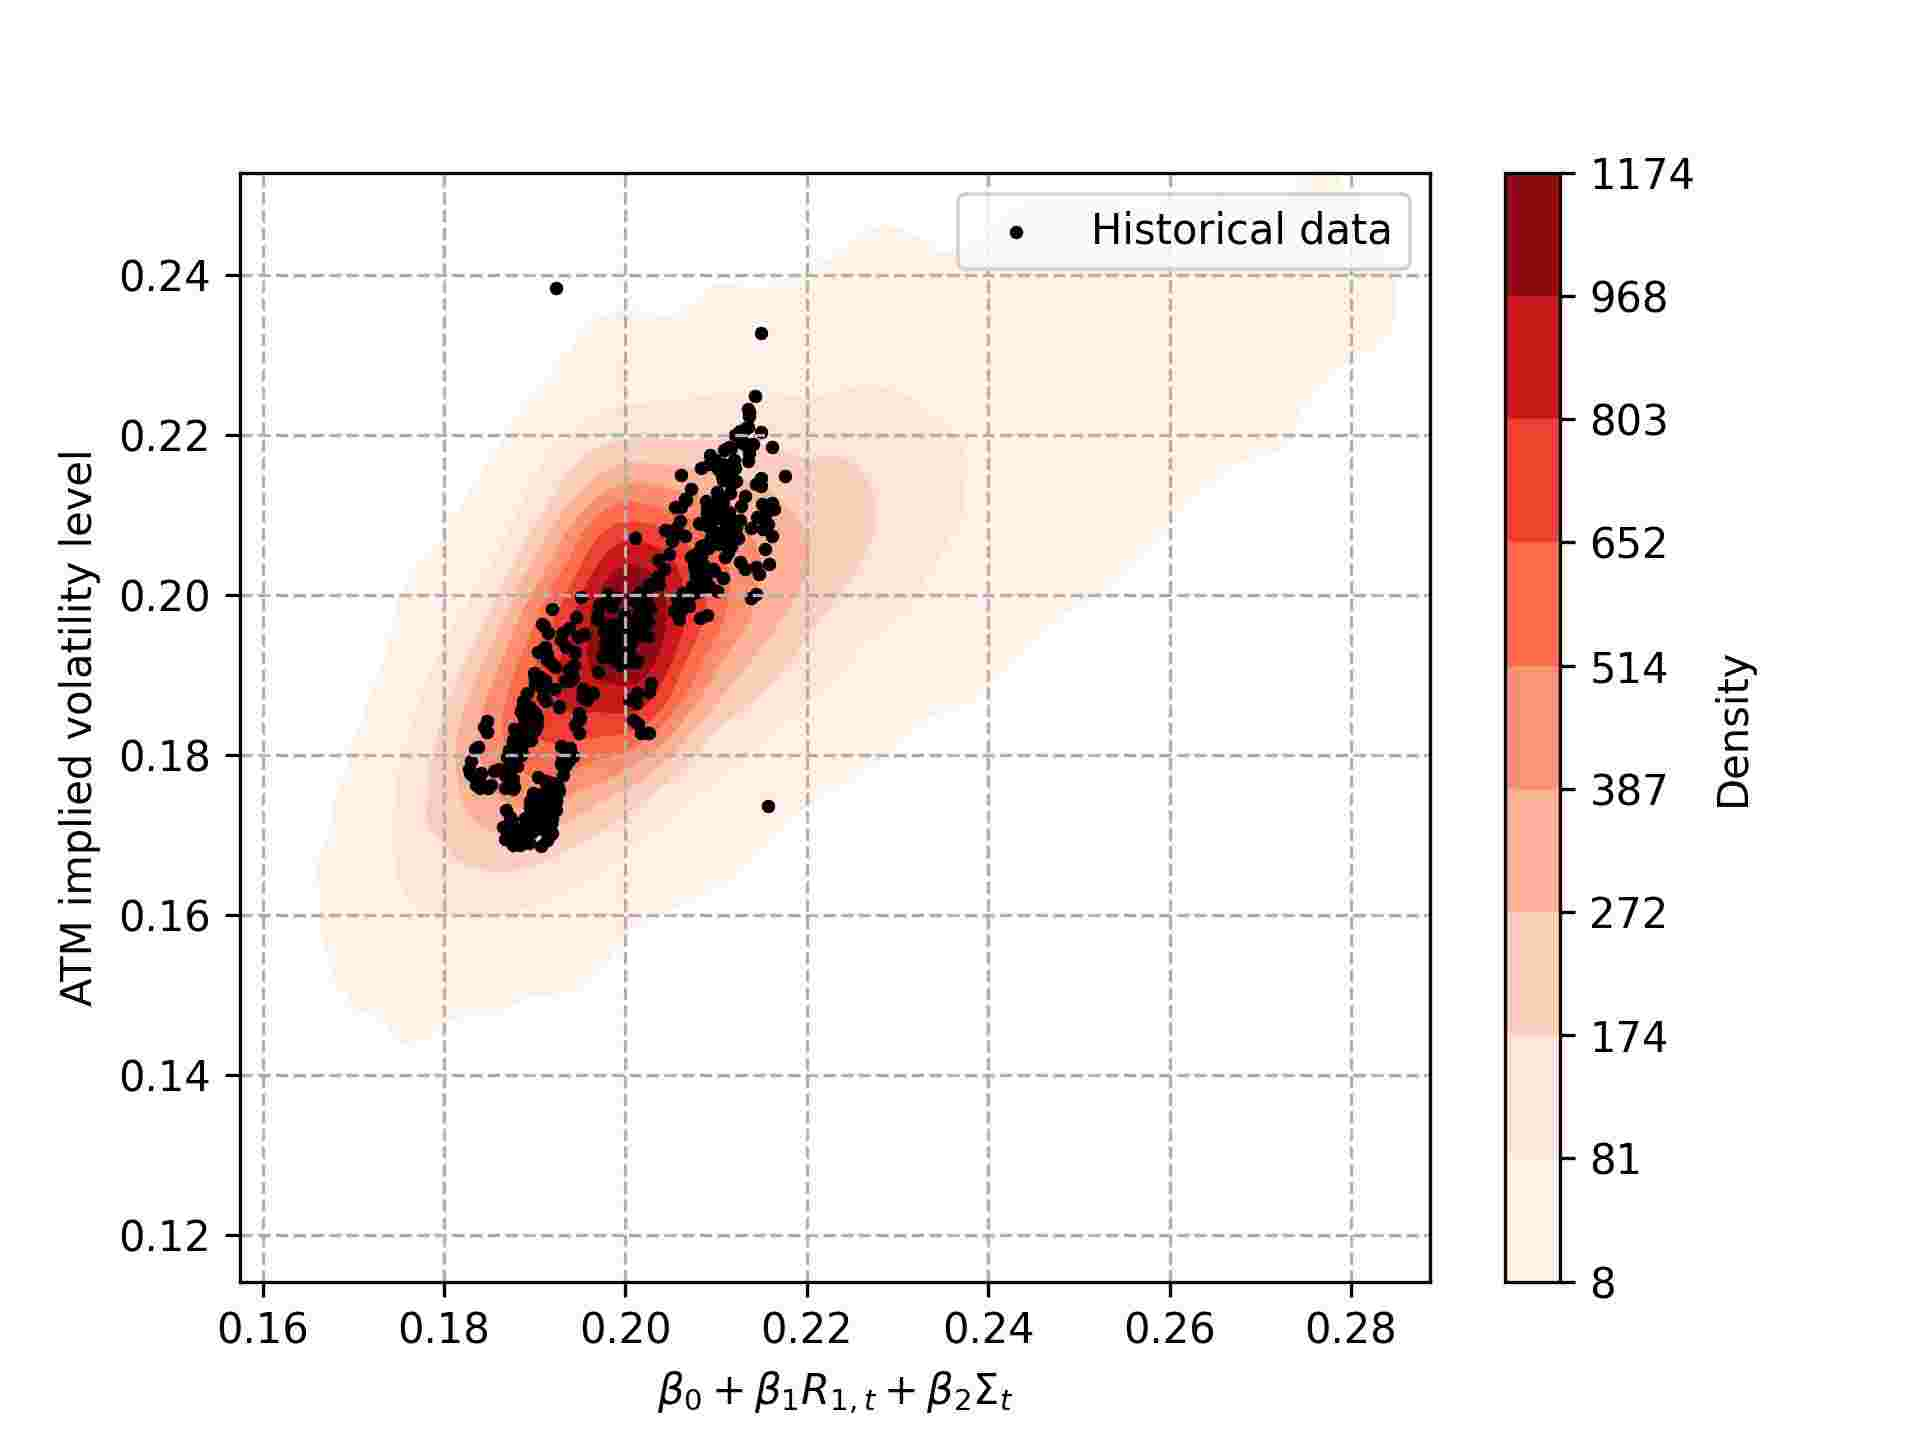
\includegraphics[width=0.3\linewidth]{STXE_KDEPlot_24M_Jacobi_Drift.jpg}}
    \caption{Joint distribution of $\beta_0+\beta_1R_{1,t}+\beta_2\Sigma_{t}$ and the ATM implied volatility level for several time-to-maturities. The black dots represents the historical realizations of these quantities.   }
\label{fig:kde_plots}
\end{figure}
To conclude this section, we compare the results from a principal component analysis (PCA) performed on the historical train set to the ones obtained from a PCA performed on the simulated IVSs. More specifically, in the same vein as \cite{cont2002dynamics}  and \cite{cont2022simulation}, we apply a PCA to the log-variations of the implied volatility on a time-to-maturity $\times$ moneyness grid. The time-to-maturities range from 1 month to 24 months with a monthly timestep while the values of the moneyness depend on each data set. For the S\&P 500, we select the values of the moneyness for which the Black-Scholes delta of a call option is historically always between 0.1 and 0.9 (consistently with the calibration of the parsimonious SSVI parameters, see Appendix \ref{sec:ssvi_calibration_results}). For the Euro Stoxx 50, the moneyness grid consists in the Black-Scholes delta grid on which the historical data is available (see Section \ref{sec:data}). In Table \ref{tab:explained_variance}, we first present the variance explained by the first four eigenvectors of the historical and simulated covariance matrices of the daily log-variations in implied volatilities on the aforementioned grid. To get these results on the simulations of the path-dependent SSVI model, 
\begin{enumerate}
    \item we apply the PCA to each simulated path,
    \item we compute the variance explained by the first four eigenvectors for each path,
    \item we average the variance explained over the 1000 paths. 
\end{enumerate}
We observe that the variance explained by the first eigenvector is similar between the PCA on historical data and the PCA on simulations, whereas the variance explained by the subsequent eigenvectors shows greater differences between the two PCAs. To complete this analysis, we also compare the shape of the two first historical eigenvectors to the two first average simulated eigenvectors in Figures \ref{fig:first_eigenvector} and \ref{fig:second_eigenvector}. We observe very similar shapes in the two Figures. In particular, we remark that:
\begin{enumerate}
    \item the first eigenvector captures the fact that the implied volatility at small time-to-maturities experiences larger variations than the one at larger time-to-maturitie,
    \item the second eigenvector captures the fact that the IVS term structure tends to flatten out when the short-term implied volatility is increasing. 
\end{enumerate}
We also compared the shapes of the third and fourth eigenvectors but they were quite different. However, as we have seen, they represent only a small part of the explained variance of the log-variations covariance matrix. Since, the two first eigenvectors explain more than 86\% (resp. 91\%) of the variance of the S\&P 500 (resp. Euro Stoxx 50) log-variations, we deduce that our model allows to capture a large part of the movements observed historically in the IVS. 


\begin{table}[]
    \centering
    \caption{Variance explained by the first four eigenvectors of the covariance matrix of the daily log-variations of the implied volatilities.}
    \label{tab:explained_variance}
    \begin{tabular}{@{}ccccccccc@{}}
    \toprule
     & \multicolumn{4}{c}{S\&P 500} & \multicolumn{4}{c}{Euro Stoxx 50} \\ \midrule
    Eigenvector & 1     & 2        & 3        & 4&  1        &   2       &   3  &4      \\\midrule
    Variance explained (historical) & 76.17\%
     & 9.88\%        & 3.69\%        &  2.14\%       &  87.25\%         &  4.22\%         &   1.54\%& 1.11\%        \\
    Variance explained (simulations) &  71.39\%       &   19.5\%      &   8.96\%      &    0.1\%       &    89.00\%        & 9.50\% & 1.23\% & 0.27\%          \\ \bottomrule
    \end{tabular}
\end{table}

\begin{figure}
    \centering
    \subfigure[Historical (S\&P 500)]{ 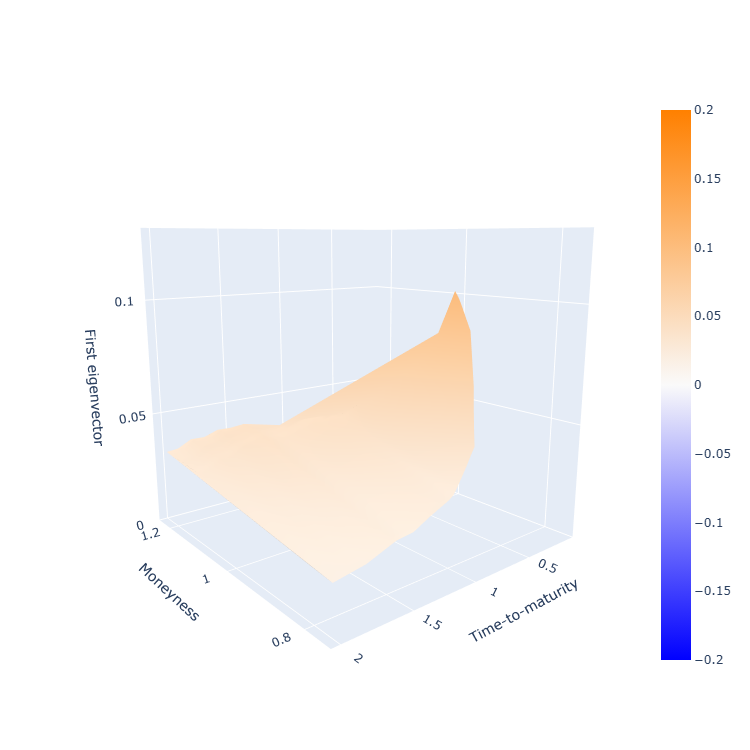
\includegraphics[width=0.45\linewidth]{SPX_Hist_Eigenvector_1.png}}
    \subfigure[Simulated (S\&P 500)]{ 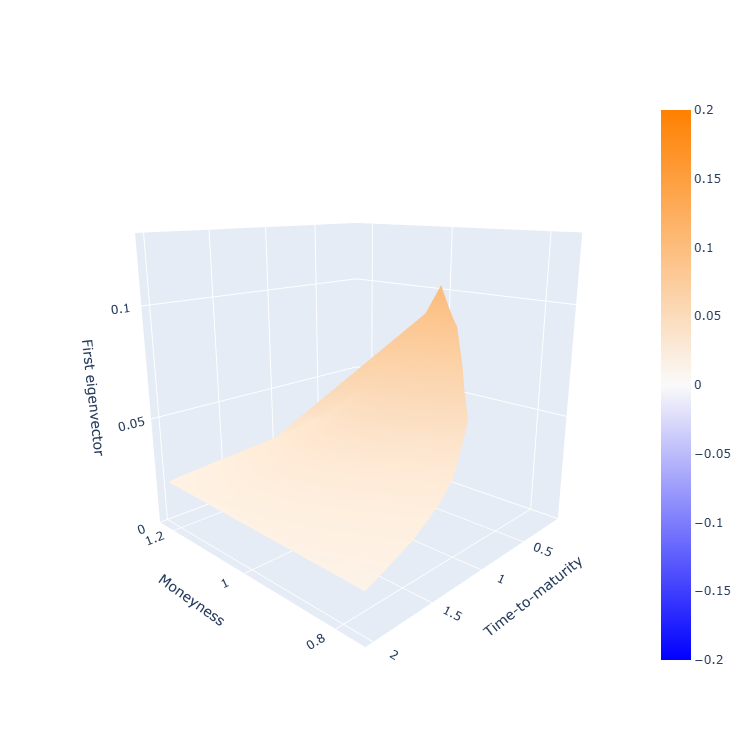
\includegraphics[width=0.45\linewidth]{SPX_Simus_Eigenvector_1.png}}

    \subfigure[Historical (Euro Stoxx 50)]{ 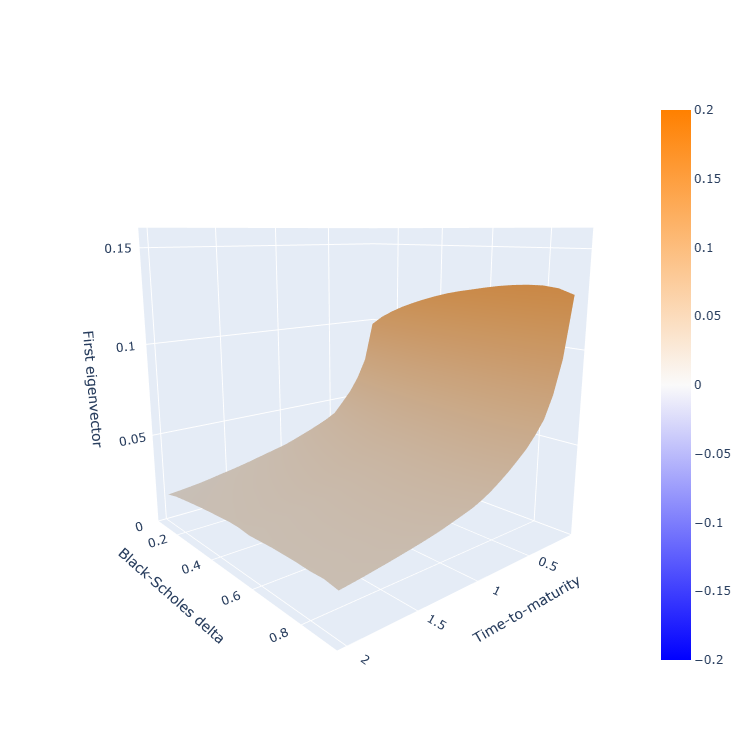
\includegraphics[width=0.45\linewidth]{STXE_Hist_Eigenvector_1.png}}
    \subfigure[Simulated (Euro Stoxx 50)]{ 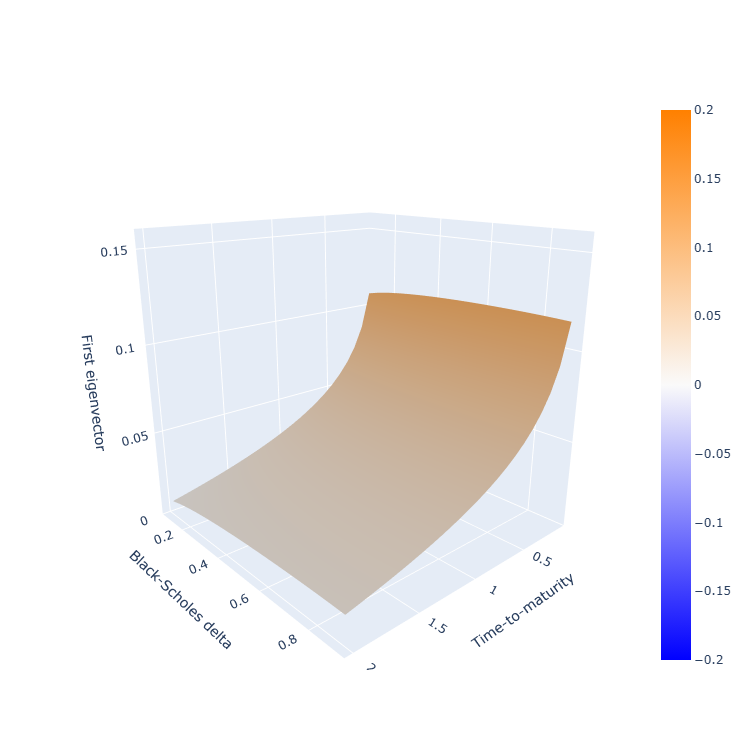
\includegraphics[width=0.45\linewidth]{STXE_Simus_Eigenvector_1.png}}
    \caption{Comparison between the first eigenvector of the PCA on the historical train set and the average first eigenvector of the PCA on the simulations.  }
\label{fig:first_eigenvector}
\end{figure}

\begin{figure}
    \centering
    \subfigure[Historical (S\&P 500)]{ 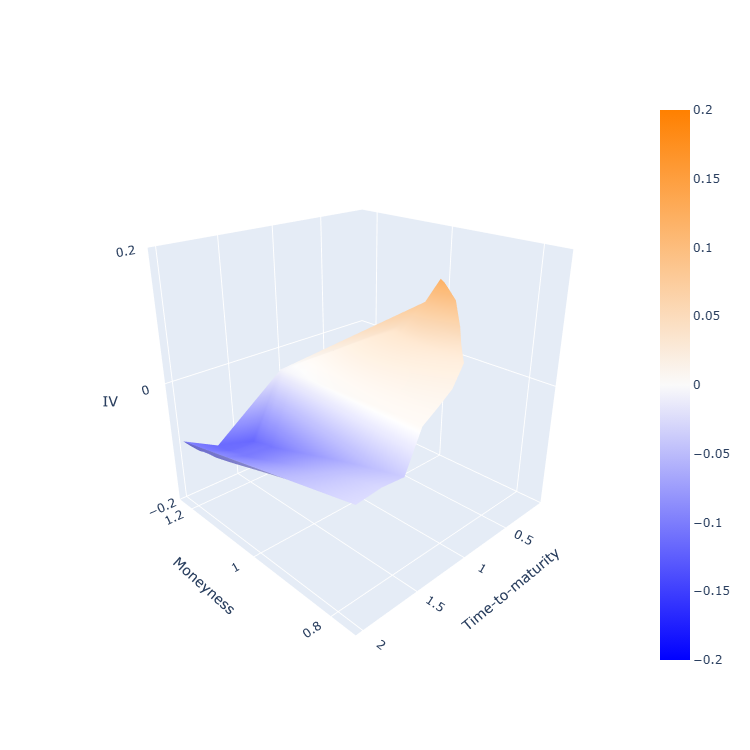
\includegraphics[width=0.45\linewidth]{SPX_Hist_Eigenvector_2.png}}
    \subfigure[Simulated (S\&P 500)]{ 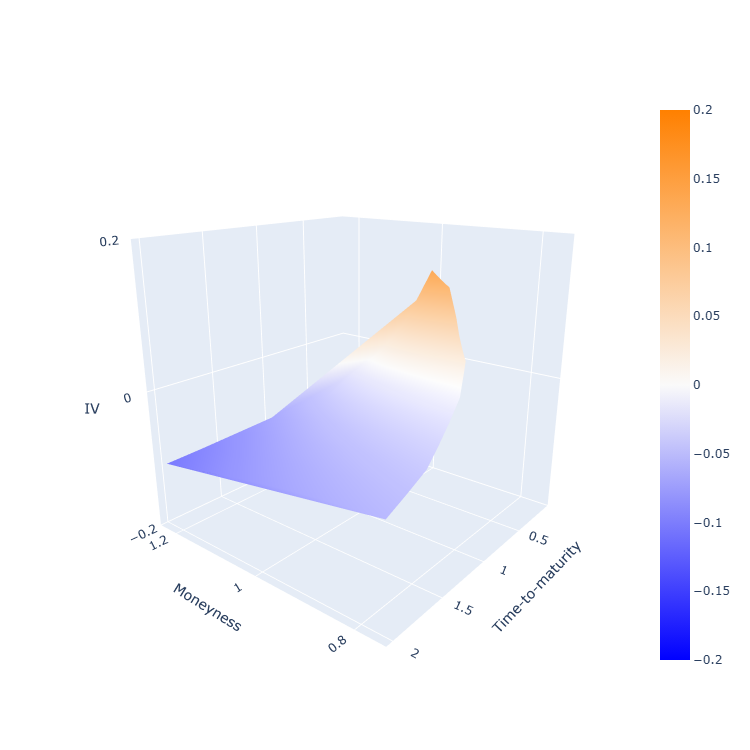
\includegraphics[width=0.45\linewidth]{SPX_Simus_Eigenvector_2.png}}

    \subfigure[Historical (Euro Stoxx 50)]{ 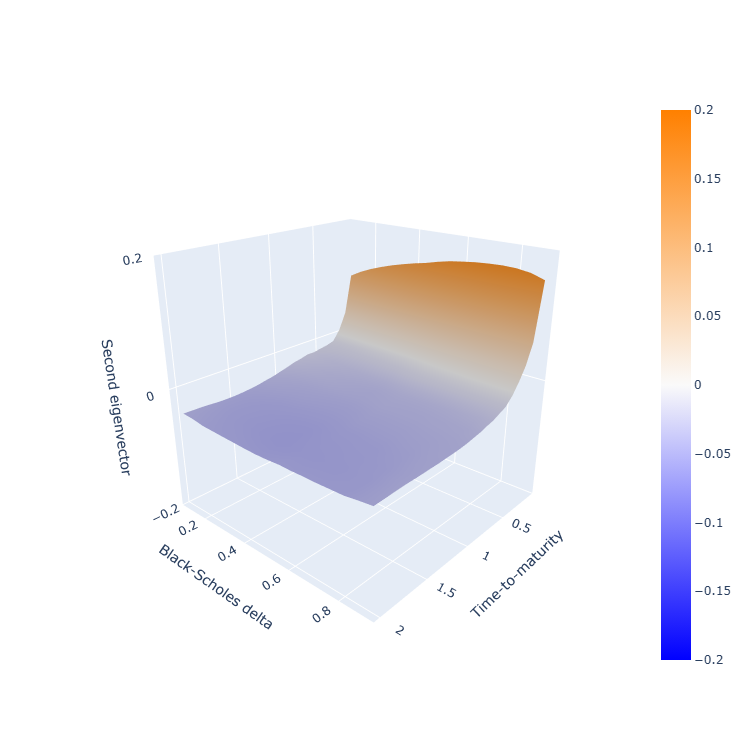
\includegraphics[width=0.45\linewidth]{STXE_Hist_Eigenvector_2.png}}
    \subfigure[Simulated (Euro Stoxx 50)]{ 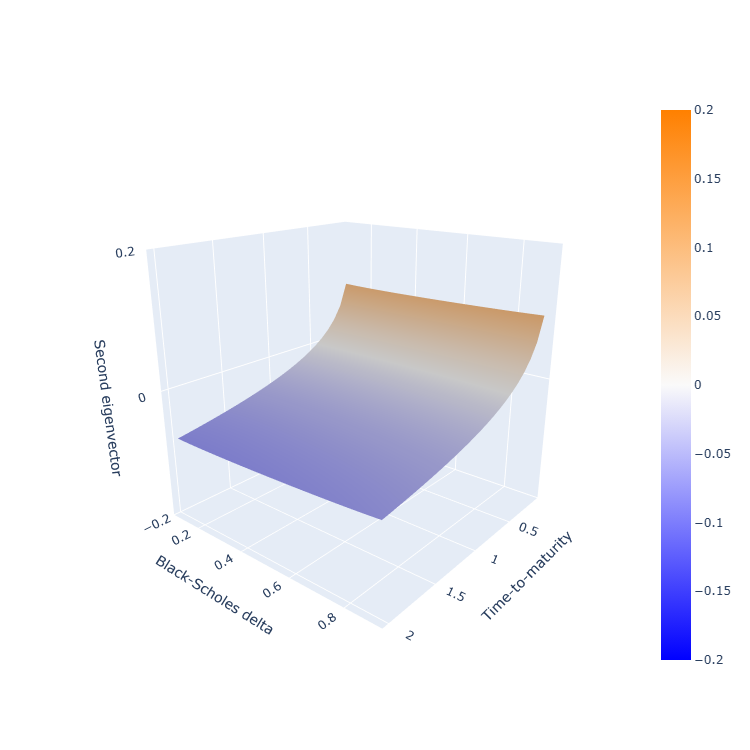
\includegraphics[width=0.45\linewidth]{STXE_Simus_Eigenvector_2.png}}
    \caption{Comparison between the second eigenvector of the PCA on the historical train set and the average second eigenvector of the PCA on the simulations.} 
\label{fig:second_eigenvector}
\end{figure}


\subsubsection{Computational cost}
 Running 1000 simulations over an horizon of 2 years with a daily time step takes approximately 2.5 minutes for 24 time-to-maturities and 81 values of moneyness on a computer equipped with an Intel Core i7-11850H, 16 cores, 2.5GHz. The model is implemented in the Python programming language. 
